\documentclass[a4paper,12pt]{article}
\usepackage[margin=0.5in]{geometry}
 
\usepackage{microtype}
\usepackage{subcaption}
\usepackage{float}

\usepackage{amsmath}
\usepackage{index}
\usepackage{graphicx}
\usepackage{hyperref}
\hypersetup{
    colorlinks=true,
    linkcolor=blue,
    filecolor=magenta,      
    urlcolor=blue,
}
\title{\Large{\textbf{Machine Learning Assignment 1 Classification Algorithms }}}
\author{Dheeraj Ramchandani}
 
 
\graphicspath{ {../plots/}}  

\begin{document}

\maketitle
\tableofcontents
%\pagenumbering{gobble}
\newpage


\section{ Kmeans Clustering   } 
\textbf{ Breast Cancer Data set} 
The second dataset is breast cancer data set taken from the UCI machine learning repository where the input data contains 30 attributes and objective of the classifier is to detect the cancer whether it is benign or malignant. This dataset is a classic dataset used by many researchers and scientists. The data set contains 569 instances ( 357 benign and 212 malignant ) where each instance represent FNA test measurement for one diagnosis case. The 30 features are computations of the 10 real valued features with their mean, standard error and mean of the 3 largest values for each nucleus cell respectively.\newline
\textbf{ Clustering Analysis } IN clustering two types of clustering is done Kmeans and Expectation maximisation.  The Kmeans  is implicitly based on the distance function to determine which points belongs to which cluster in contrast  EM uses probability distribution to determine the number of components. In the Kmeans Euclidean distance is used for the clustering, to find the number of clusters we have used the silhouette analysis and inertia analysis. Inertia analysis measures the error which is the distance of the each of the point from the cluster( centroid ) and the analysis is called the elbow analysis and the number of clusters is the point where the elbow bends and so from the graph we can see that the number of clusters for this dataset is 2. \newline

\textbf{Silhouette Analysis} S.A. is a way to measure how close each point in a cluster is to the points in its neighboring clusters. Its a neat way to find out the optimum value for k during k-means clustering. S.A values lies in the range of -1 to +1 where the positive values is desirable and 0 means it is at the boundary and negative values indicates that the point is assigned to the wrong cluster. we did the silhouette analysis for clusters ranging from 2 to 12 and measured the values we can see that the value is maximum for clusters 2 and decreases rapidly with the increase in the clusters value.  The red doted line is the mean S score for cluster in consideration.  Following points were chosen in order to select the k value which is mean value should be as high as possible which was for k value 2 and also the width of each clusters should be as uniform as possible and each cluster should not be behind the mean value, so after considering all those points the k value of 2 was chosen and also it coincides with the labels in the dataset as it is a binary dataset.  As we increase the clusters some of the clusters are also behind the mean value and also the SA values decreased rapidly.\newline
\begin{figure}[!htb]
   \begin{minipage}{0.33\textwidth}
     \centering
     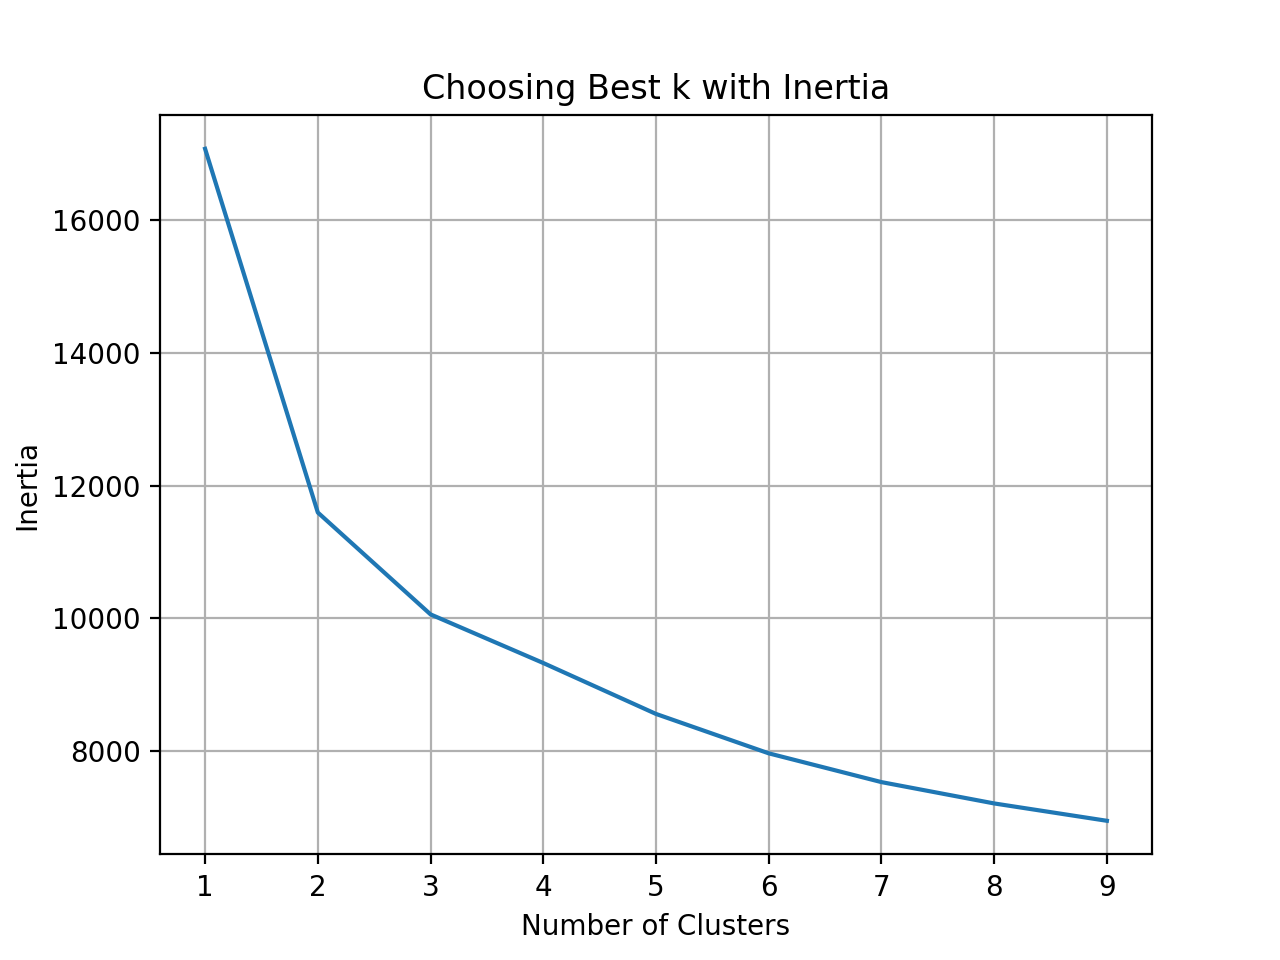
\includegraphics[width=.95\linewidth]{kmeans_inertia_1}
   \end{minipage}\hfill
    \begin{minipage}{0.33\textwidth}
     \centering
     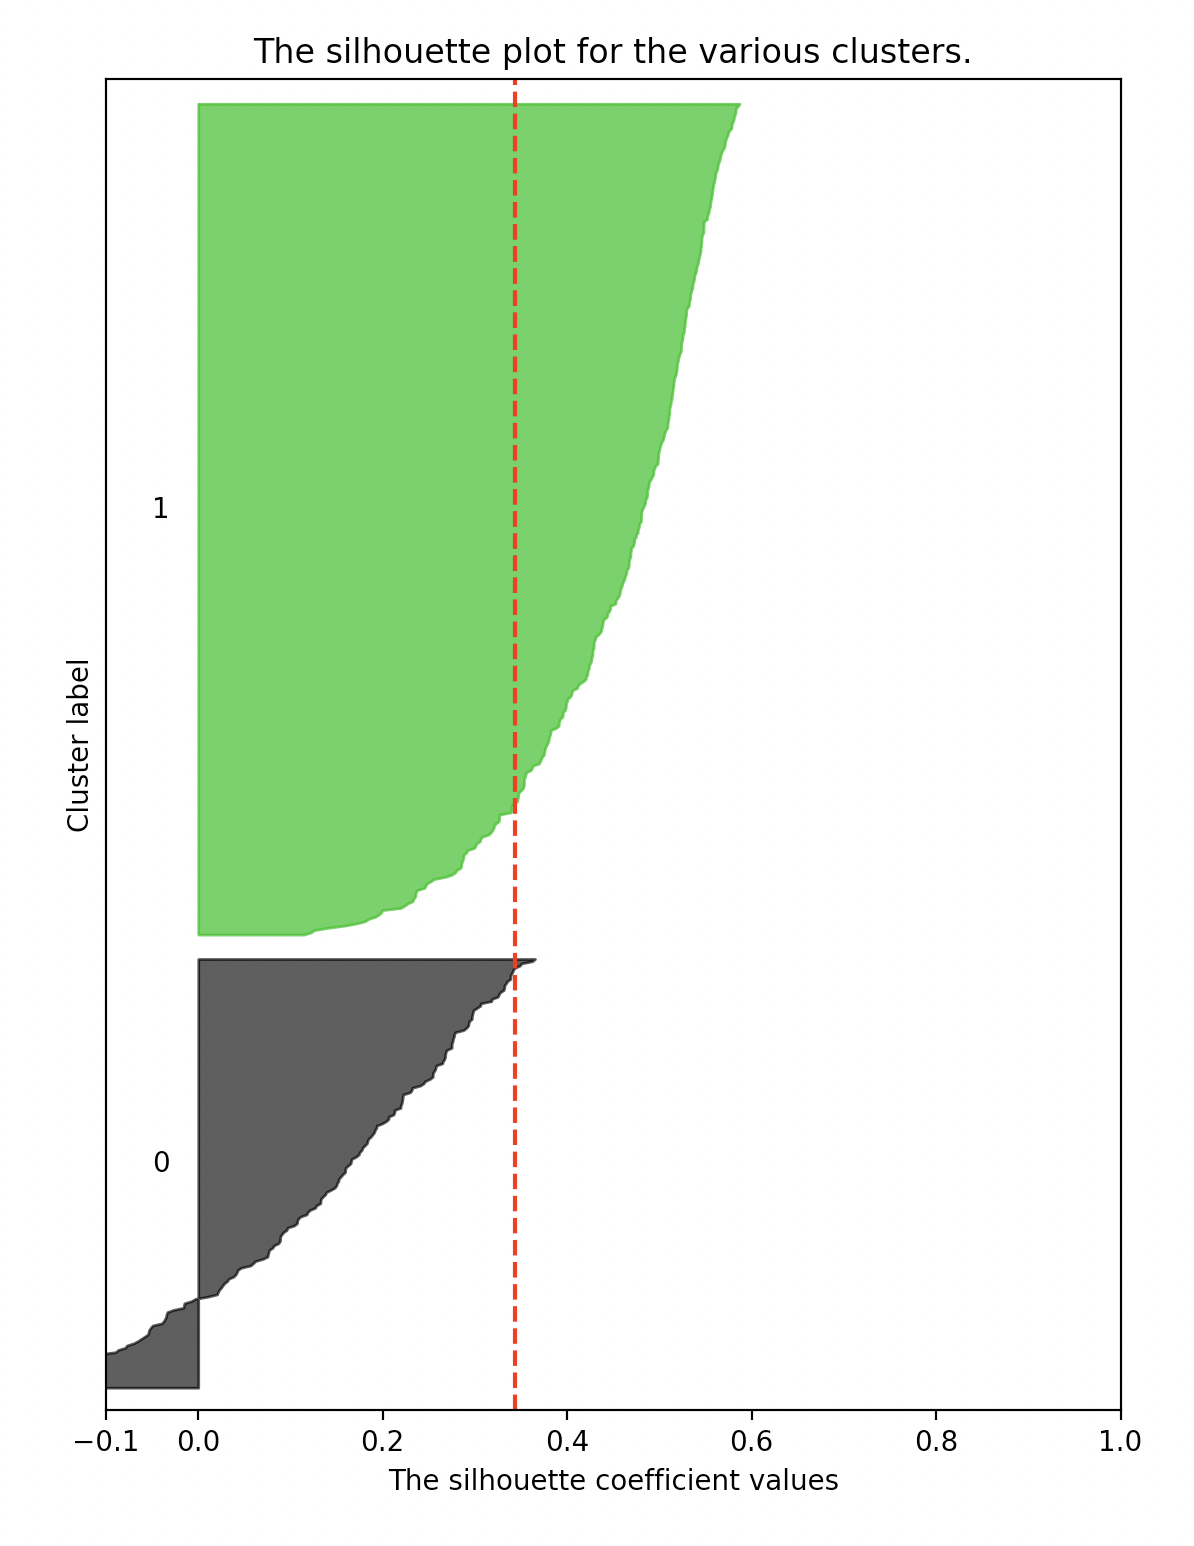
\includegraphics[width=.95\linewidth]{sil_kmeans_11}
     \end{minipage}\hfill
     \begin{minipage}{0.33\textwidth}
     \centering
     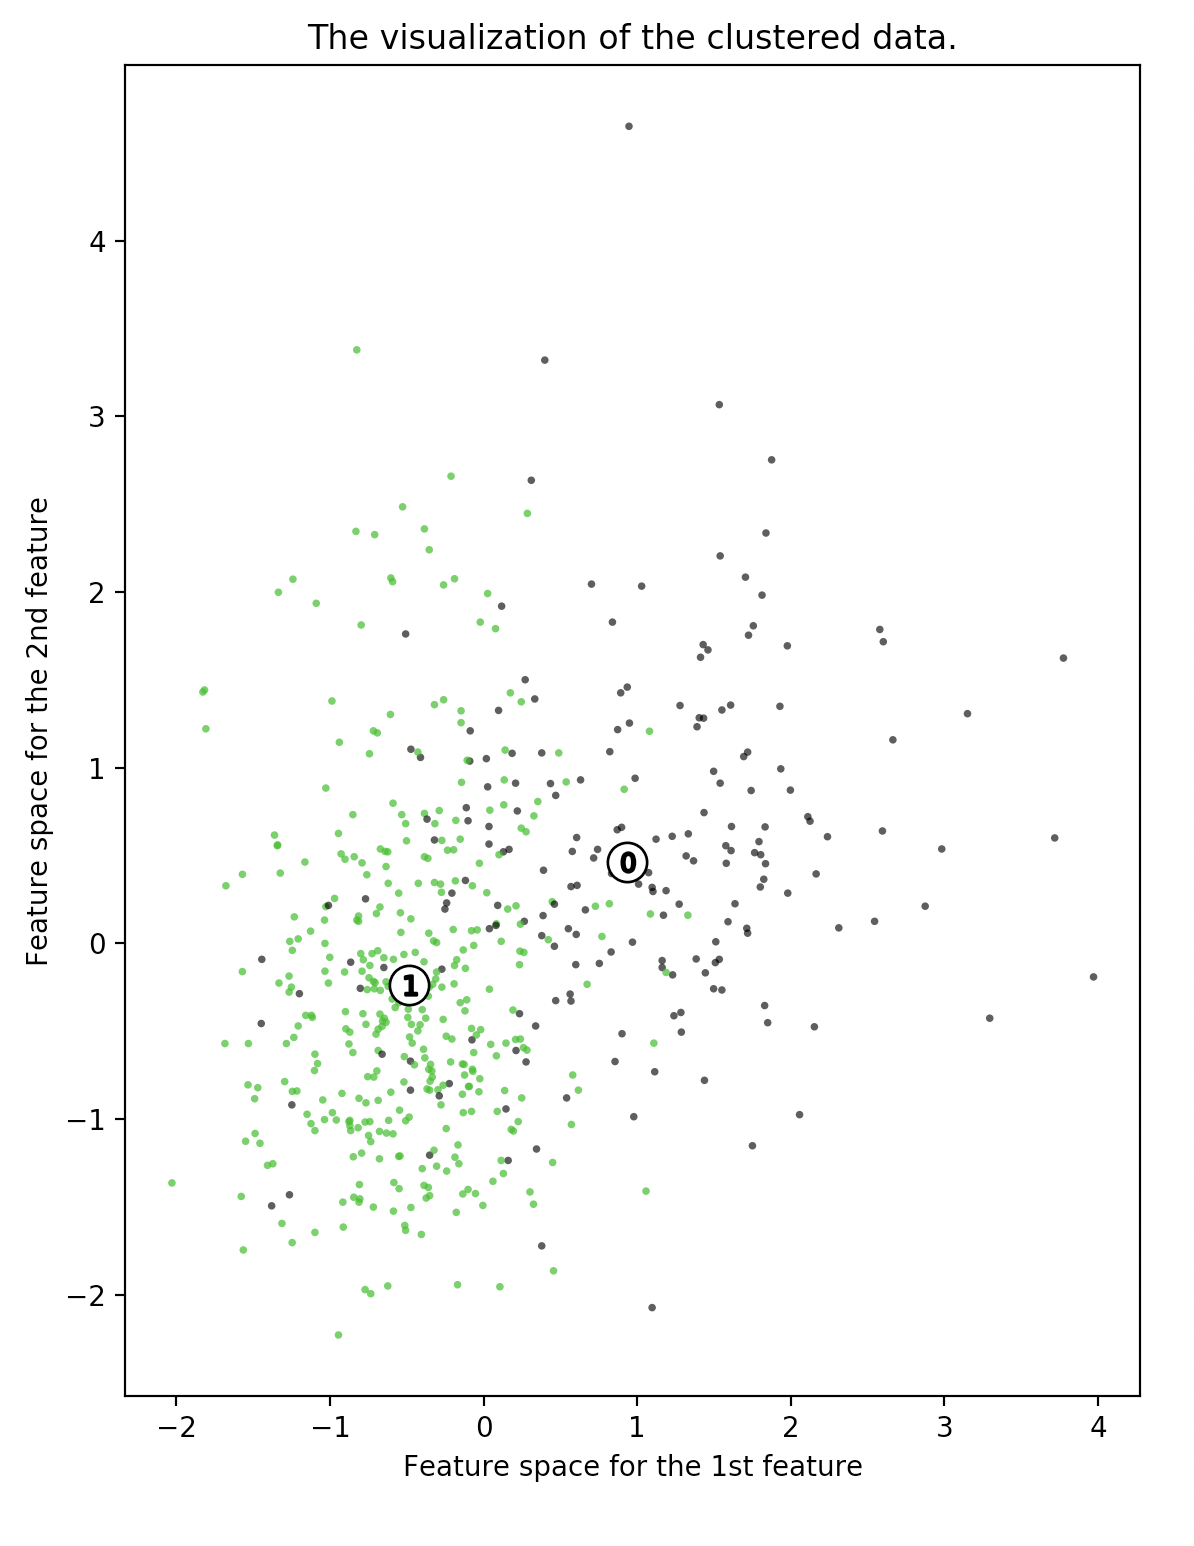
\includegraphics[width=.95\linewidth]{sil_kmeans_12}
   \end{minipage}\hfill
 \caption { Simulated Annealing Tuning}
\end{figure}


\textbf{ Quality of cluster} So in the Kmeans the number of cluster is found to be 2 and now to evaluate the quality of cluster we have used the homogenity score and the AMI ( adjusted mutual information ) score is 0.554 which is also good and also the samples in the clusters were plotted against the original labels in this data set the we can see that out of 212 malignant samples 175 are correctly matched to the cluster 0 and for benign only 14 are incorrectly matched which also supports the k value.

\begin{figure}[!htb]
   \begin{minipage}{0.33\textwidth}
     \centering
     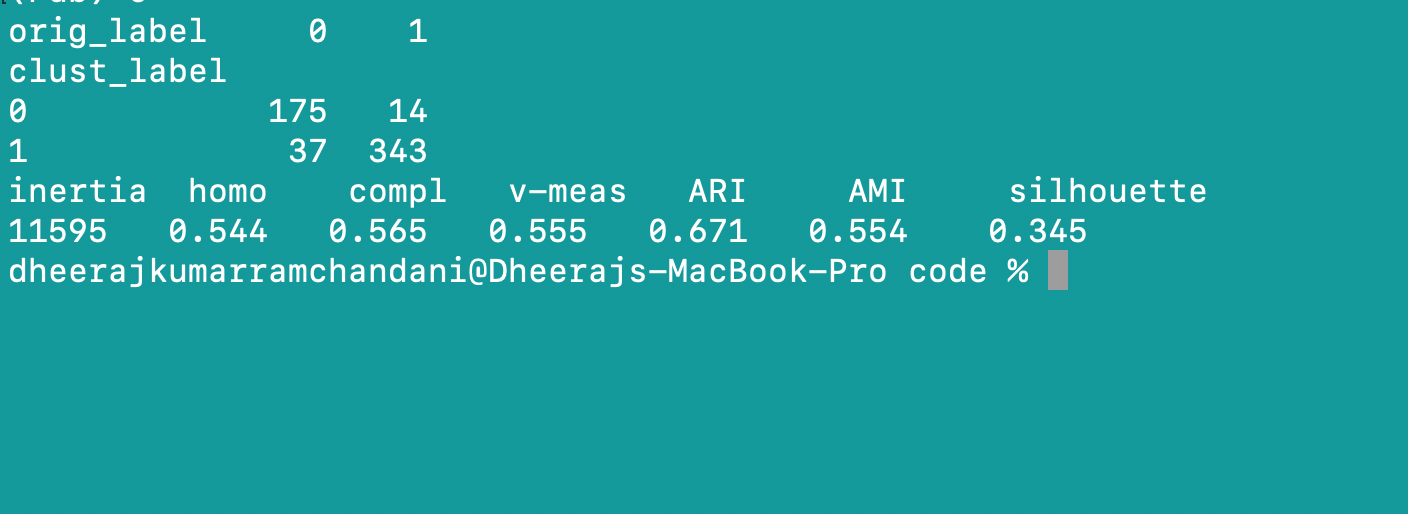
\includegraphics[width=.95\linewidth]{kmeans_cluster11}
   \end{minipage}\hfill
    \begin{minipage}{0.33\textwidth}
     \centering
     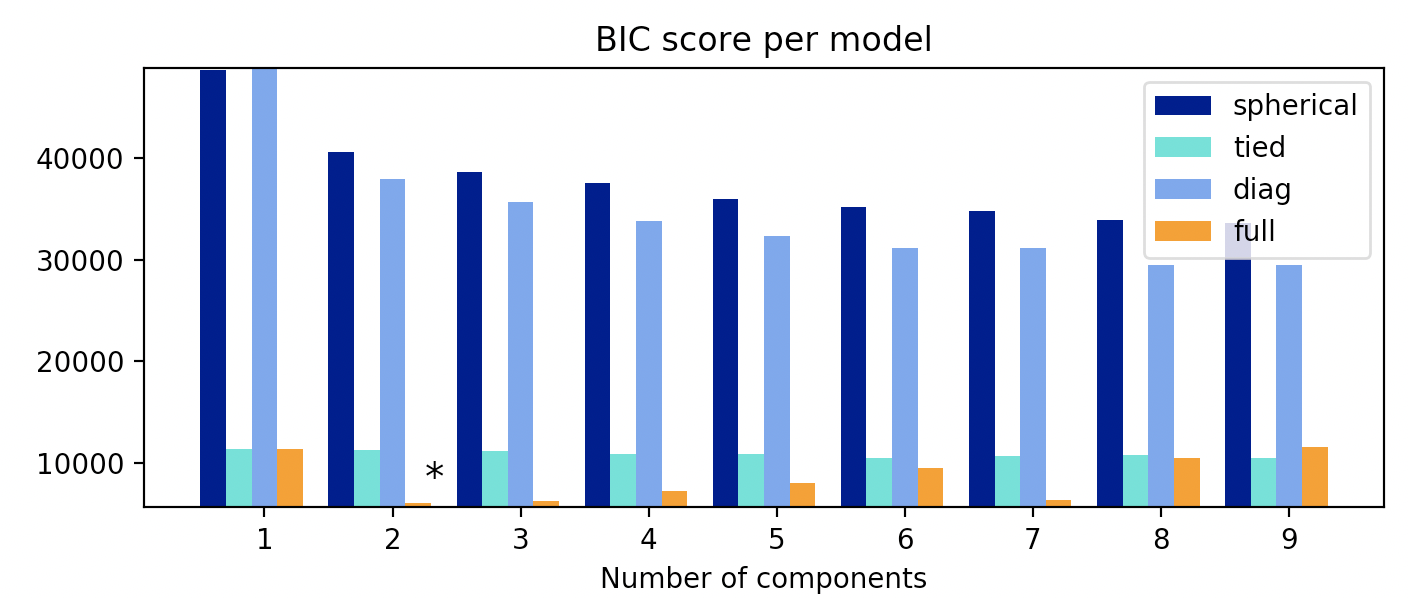
\includegraphics[width=.95\linewidth]{em_11}
     \end{minipage}\hfill
     \begin{minipage}{0.33\textwidth}
     \centering
     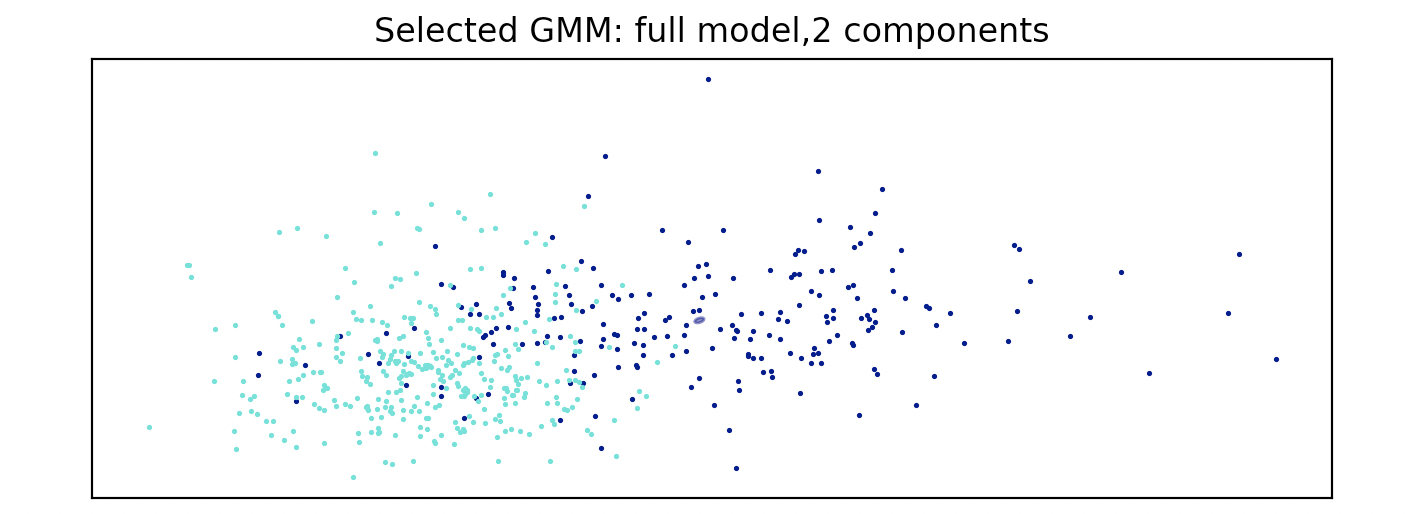
\includegraphics[width=.95\linewidth]{em_12}
   \end{minipage}\hfill
 \caption { Simulated Annealing Tuning}
\end{figure}

\textbf{ Expectation Maximisation } The expectation maximisation algorithm on the breast cancer data set is performed where the covariance type which controls the degree of freedom in the shape of each cluster is also varied from the simpler spherical to the complex full model which allows the cluster ot be modelled as an ellipse with an arbitrary orientation, the number of components were varied from 1 to 10 . It is expected that the number of components should come out to be 2. For the model selection the BIC (  Bayesian information theoretic criteria)  is followed and in the graph we can see that the BIC value is lowest for number of components as 2 and the covariance type as full which coincides with the number of labels.  The bayesian information criteria penalizes the larger number of clusters in order to avoid overfitting. The Number of clusters for the gmm was also confirmed via the silhouette analysis where we plotted the SA score for each cluster and picked the highest one and it is 2 so the number of components is 2. \newline.

\textbf{ Human Activity Data}  The data comprise labeled examples of 30 people performing six different activities: walking, climbing stairs, descending stairs, sitting, standing, and lying down. The activities within each category have similar accelerometer and gyroscope readings.
The data were gathered through a waist­mounted smartphone (specifically, a Samsung Galaxy SII released in 2011 and considered top­of­the­line for that time). The data include both accelerometer and gyroscope readings, sampled at a constant rate of 50 Hz, which were then segmented into 2.56­second windows with a window overlap of 50\%. Along with raw readings, the dataset includes filtered and derived features such as gravity acceleration separated from body acceleration via a low­pass filter, jerk, standard deviation, and cross­axis correlation.
Of the volunteer subjects, 70\% were selected randomly to contribute to the training dataset, and 30\% for the test set. In total, the training and test matrices include 561 features per data point, with data split into 7,352 training examples and 2,947 test examples.

\begin{figure}[!htb]
   \begin{minipage}{0.33\textwidth}
     \centering
     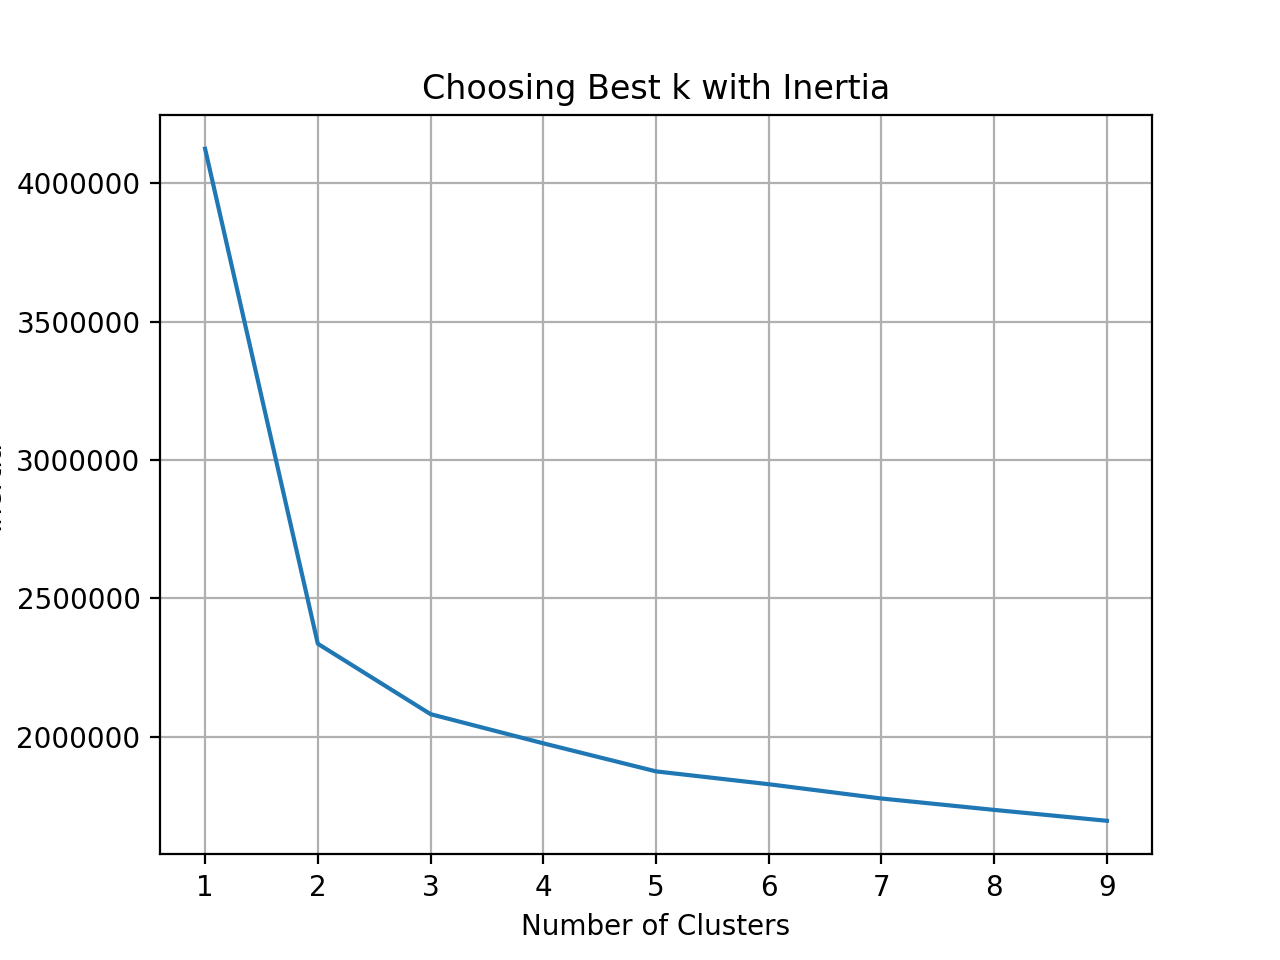
\includegraphics[width=.95\linewidth]{kmeans_inertia_2}
   \end{minipage}\hfill
    \begin{minipage}{0.33\textwidth}
     \centering
     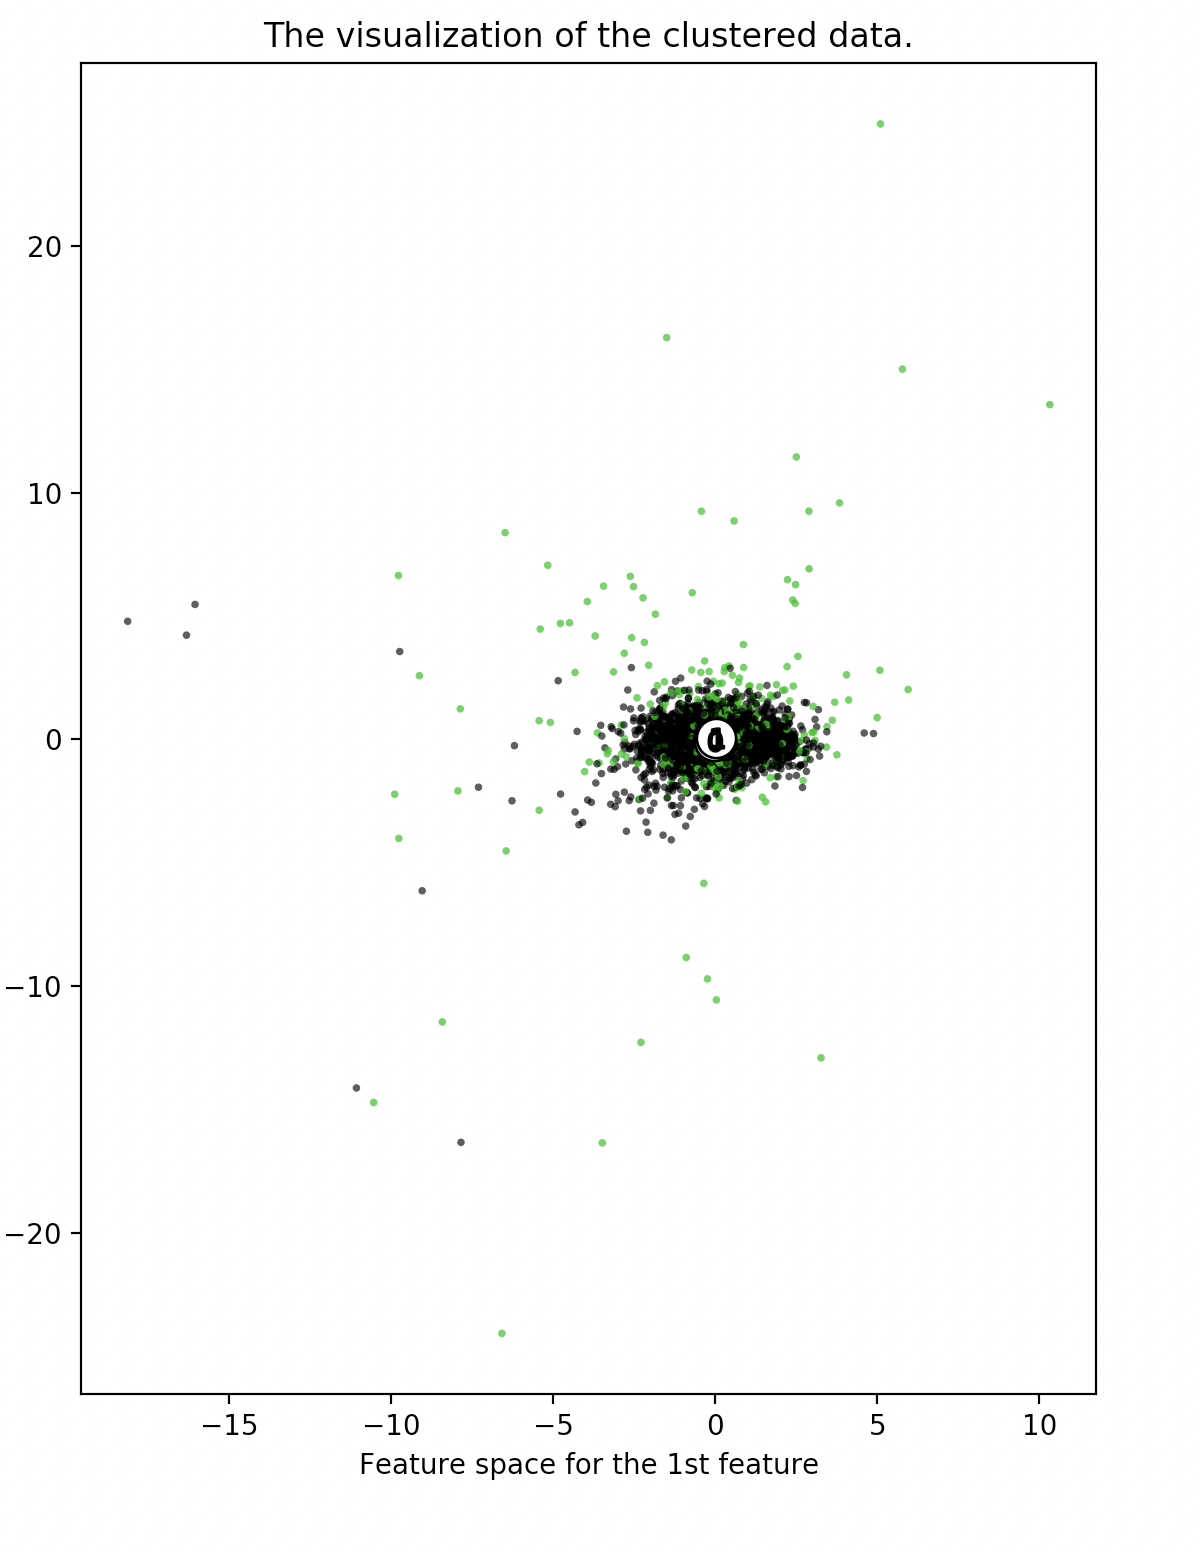
\includegraphics[width=.95\linewidth]{kmeans_sil_21}
     \end{minipage}\hfill
     \begin{minipage}{0.33\textwidth}
     \centering
     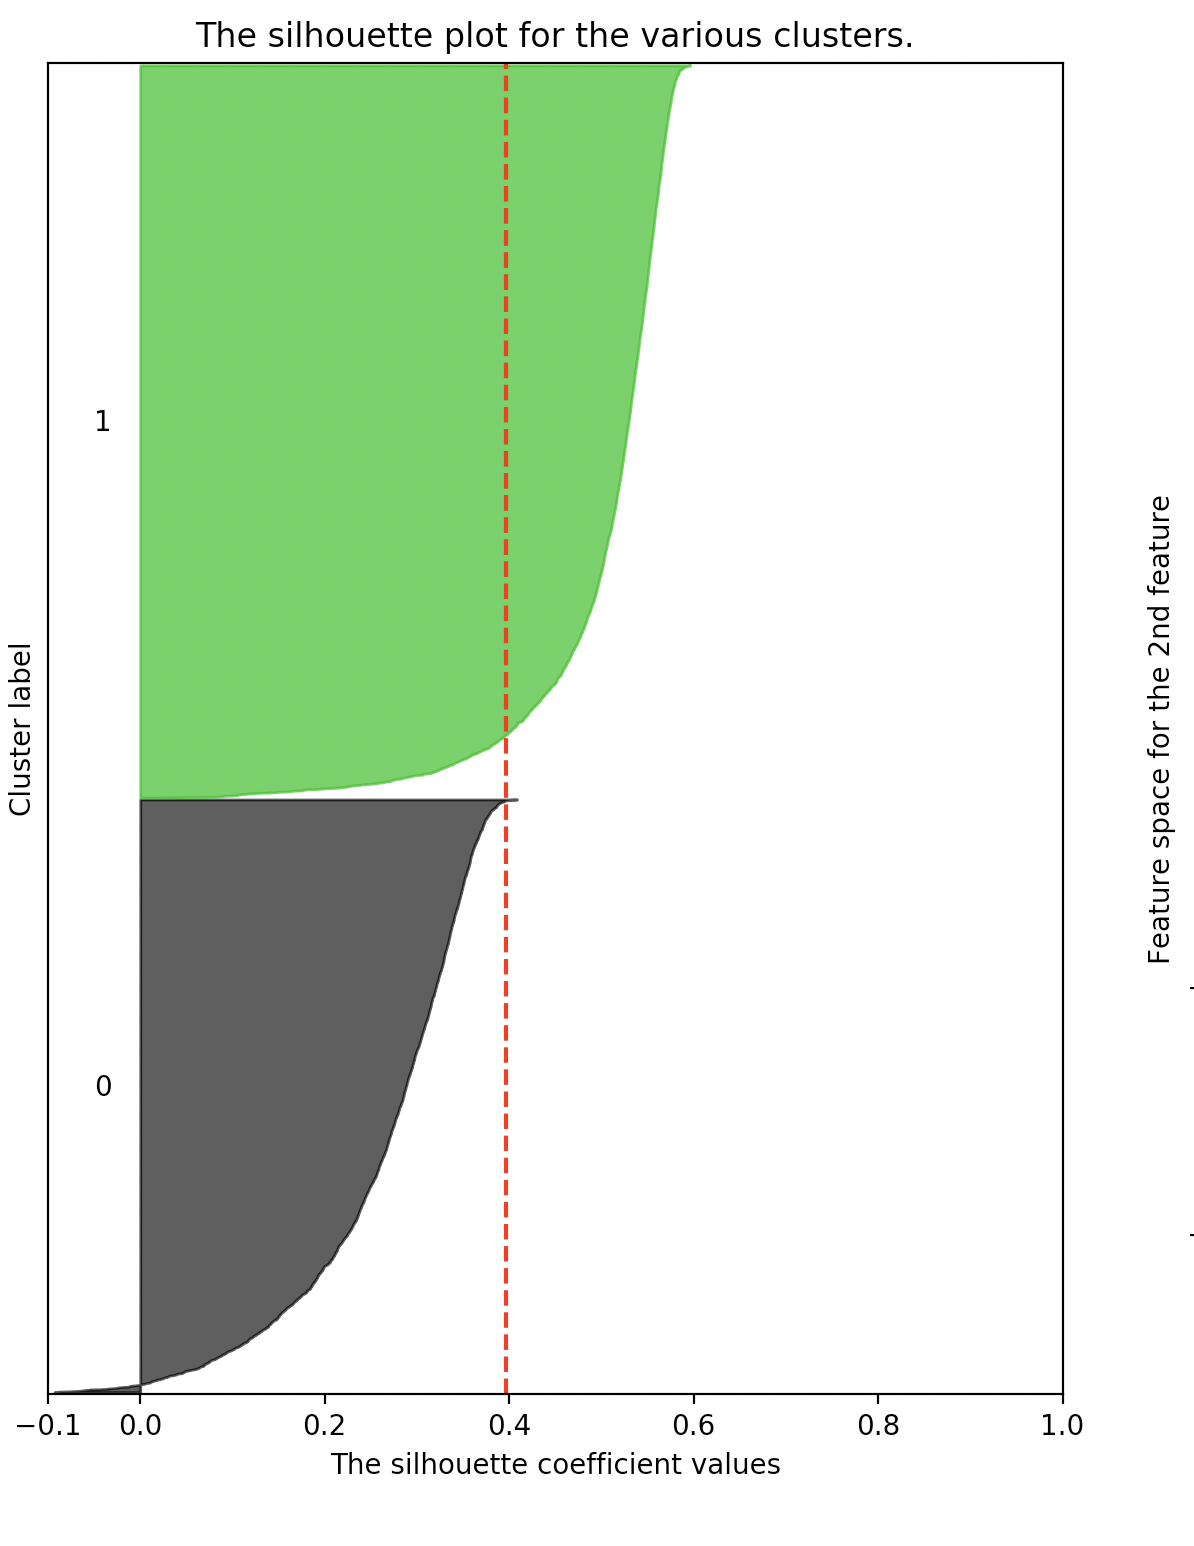
\includegraphics[width=.95\linewidth]{kmeans_sil_22}
   \end{minipage}\hfill
 \caption { Simulated Annealing Tuning}
\end{figure}
\textbf{ Kmeans Clustering} The Kmeans clustering is run on the data set and the clustering algorithm converges on the dataset with the clusters ranging from 2 to 10. The centroids were chosen randomly  and the number of iterations are fixed to be 300. \newline
\textbf{ Elbow analysis and Silhouette } When we run the elbow analysis we can see that the optimum number of the clusters for the dataset is 2 and we have also done the silhouette analysis where we  can also see that the value of SA is maximum for k=2 and then decreases rapidly from k=4 to increasing values of k. \textbf{Here the number of clusters does not coincides with the number of the labels.} we initially thought that the number of clusters will coincide with the labels but that does not happened. The clusters are found to be 2 which can be analysed as the activities are standing , sitting , laying , walking , climbing upstairs and climbing downstairs which means that the kmeans algorithm segregates between the motion activities and the sedentary activities to confirm that we checked the distribution of the samples within the cluster  for cluster values of 2 and 6. In the below figure we can see that almost all of the instances of the activities 1,2,3 goes to the cluster 1 and the activities 4, 5, 6 goes to the cluster 0.  \textbf{ For quality of cluster } we can see that the activities 1, 2, 3 were walking , climbing downstairs , climbing upstairs which are all motion activities and the activities 4,5, 6 all are sedentary activities. The correlation between the clusters and the original labels were also done for k=6 which we can see that is not good and various scores are also printed for the same which also suggests that k =2 is a better choice than k=6. The third figure below shows the SA scores for various values of k and this also suggests that k=2 is the right choice. \newline 


\begin{figure}[!htb]
   \begin{minipage}{0.33\textwidth}
     \centering
     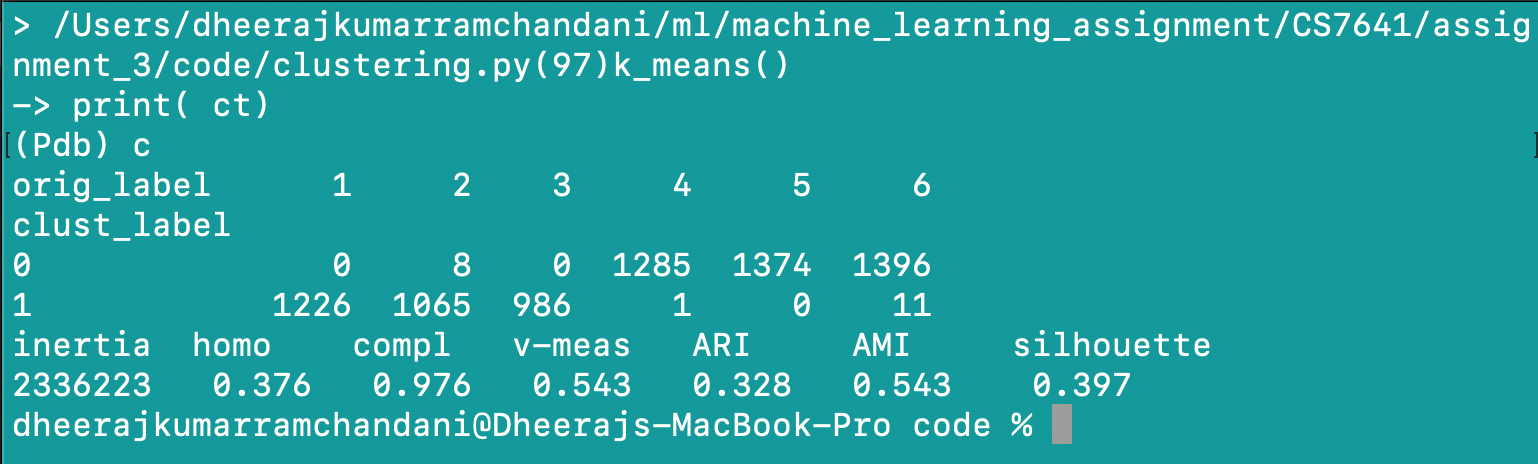
\includegraphics[width=.95\linewidth]{kmeans_cluster_21}
   \end{minipage}\hfill
    \begin{minipage}{0.33\textwidth}
     \centering
     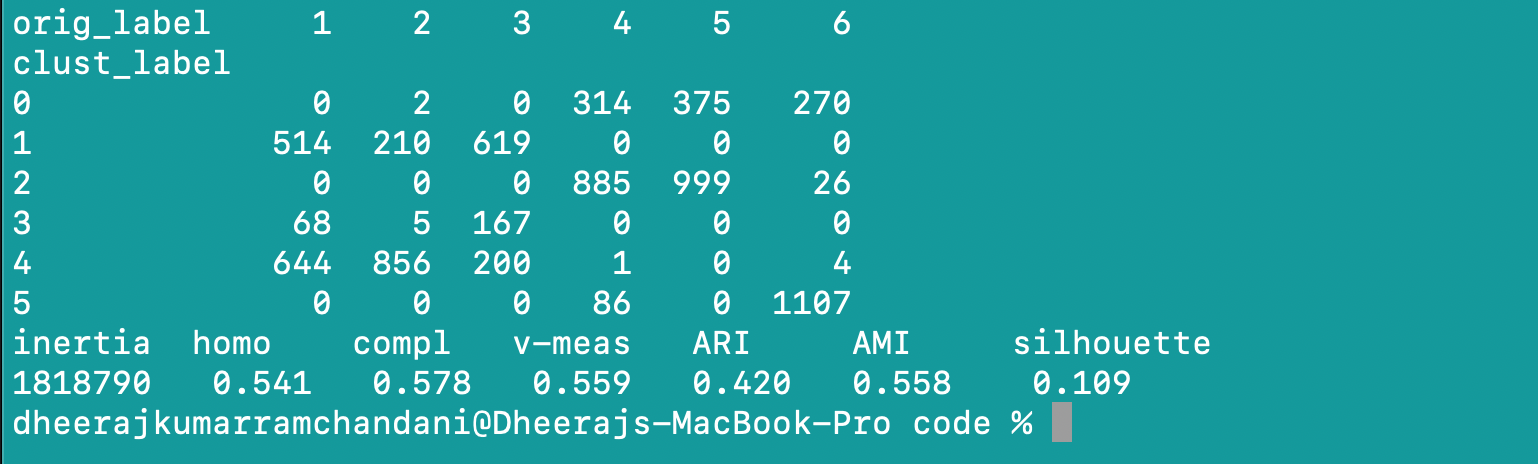
\includegraphics[width=.95\linewidth]{kmeans_cluster_22}
     \end{minipage}\hfill
     \begin{minipage}{0.33\textwidth}
     \centering
     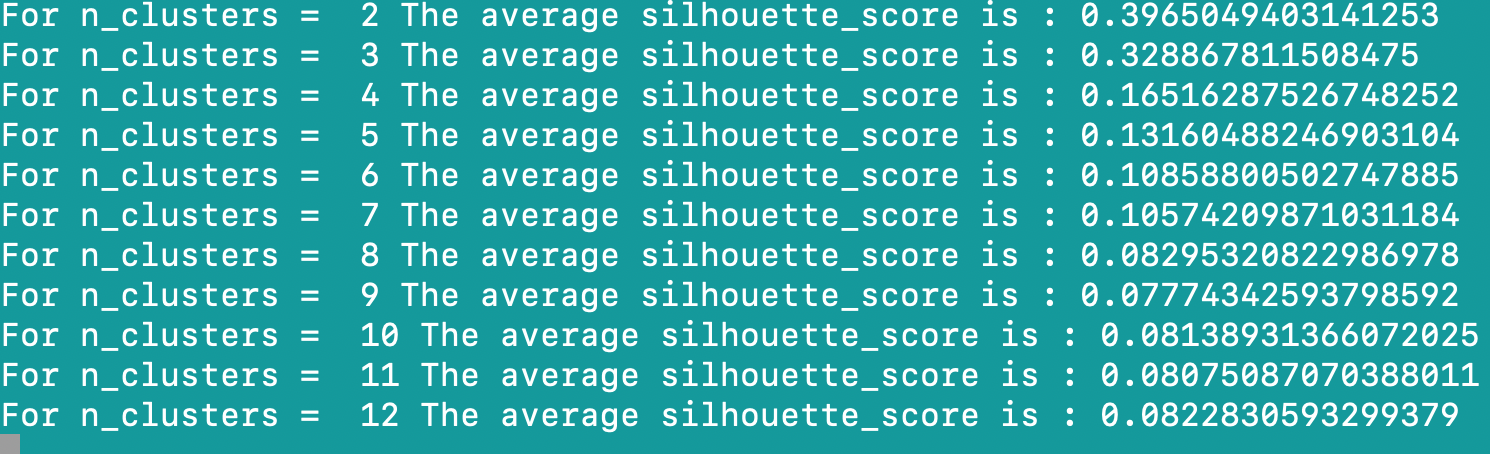
\includegraphics[width=.95\linewidth]{kmeans_sil_23}
   \end{minipage}\hfill
 \caption { Simulated Annealing Tuning}
\end{figure}

\textbf{ Expectation maximisation} The EM algorithm same setup is used as was used for the dataset 1 where the number of components were varied from 1 to 20 and the degree of freedom is varied from spherical to full. The hyper parameters to chose for this dataset is determined using the BIC analysis which ever configuration minimises the value is chosen. here we can see that the number of components is found to be 2 and the covariance type to be full which coincides with the result we got with the kmeans also.


\section {PCA} 
PCA which is the principle component analysis used in many areas such as noise reduction, feature extraction , dimensionality reduction. The principle components are the directions of the maximum variance and the components with least variance can be dropped which can solve the curse of dimensionality. To decide the number of components to keep after the dimensionality reduction  elbow analysis was used  on the reconstruction plot and also the plot showing the cumulative  variance gained with the number of components.  \newline
\textbf{ Data set1 } For the dataset 1 from the reconstruction we got the number of components to be 6 and also from the variance plot the 6 components account for 93 percent of variance so noc for the first dataset was selected 6, here the first 2 components account for 74 percent of variance so noc 6 is appropriate. We need 10 principal components to explain more than 0.95 of the variance and 17 to explain more than 0.99 \newline 
  \textbf{ Data set 1 visualisation using PCA} For better data visualization of the boundaries of the dataset we have also tried with number of components as 2 which is also decent we have seen that the first two components account for around 73 percent of the variance we can use these two and will still be able to distinguish the cancer between benign and malignant. We have selected only 2 components and that will be orthogonal to each other,  to understand how the original features got mixed to create the components we also created a heat map which showed the contribution of each feature to the components. That figure is also shown which shows that

\begin{figure}[!htb]
   \begin{minipage}{0.33\textwidth}
     \centering
     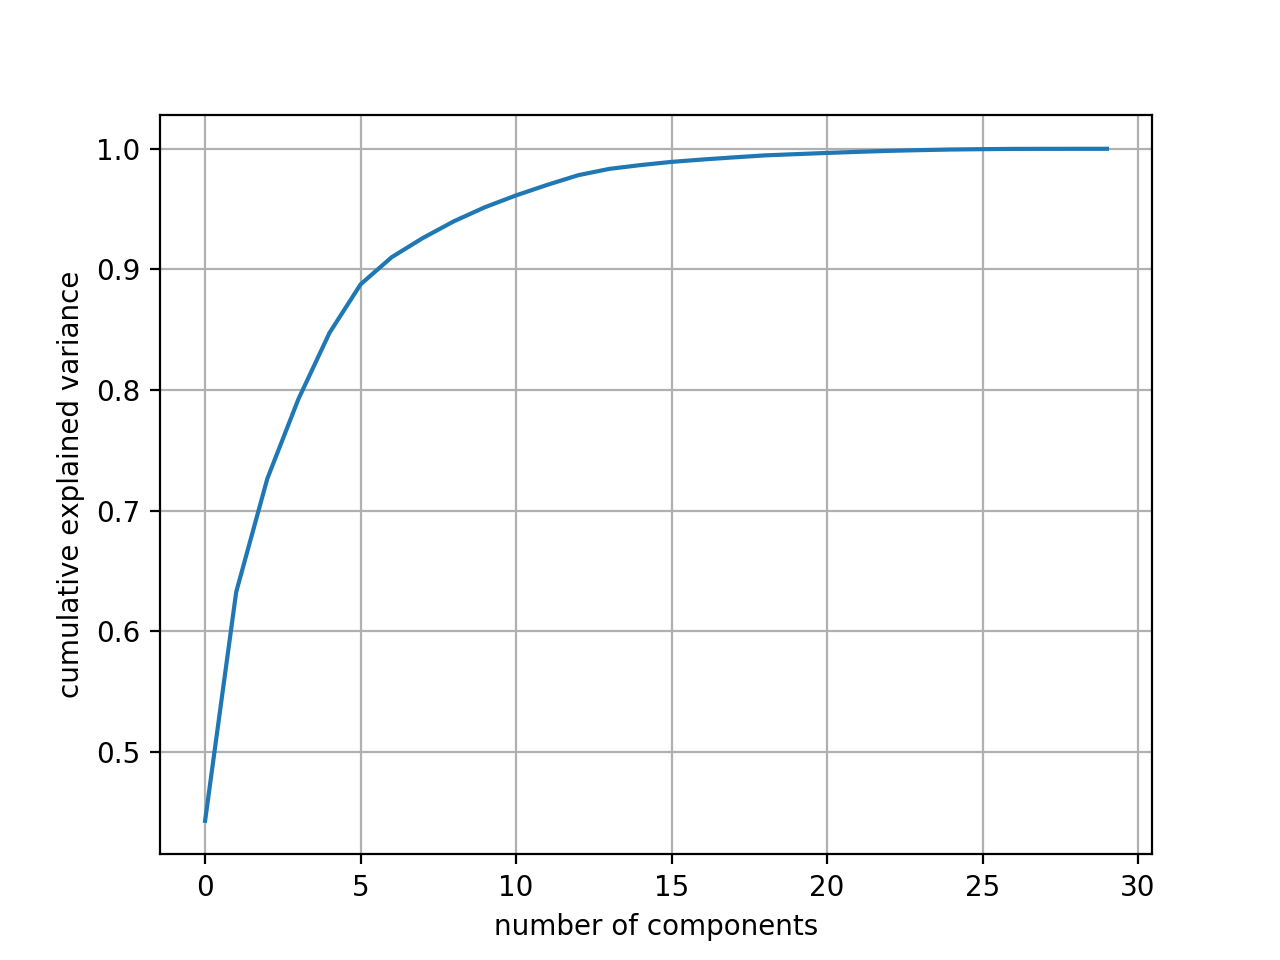
\includegraphics[width=.95\linewidth]{pca_data_set11}
   \end{minipage}\hfill
    \begin{minipage}{0.33\textwidth}
     \centering
     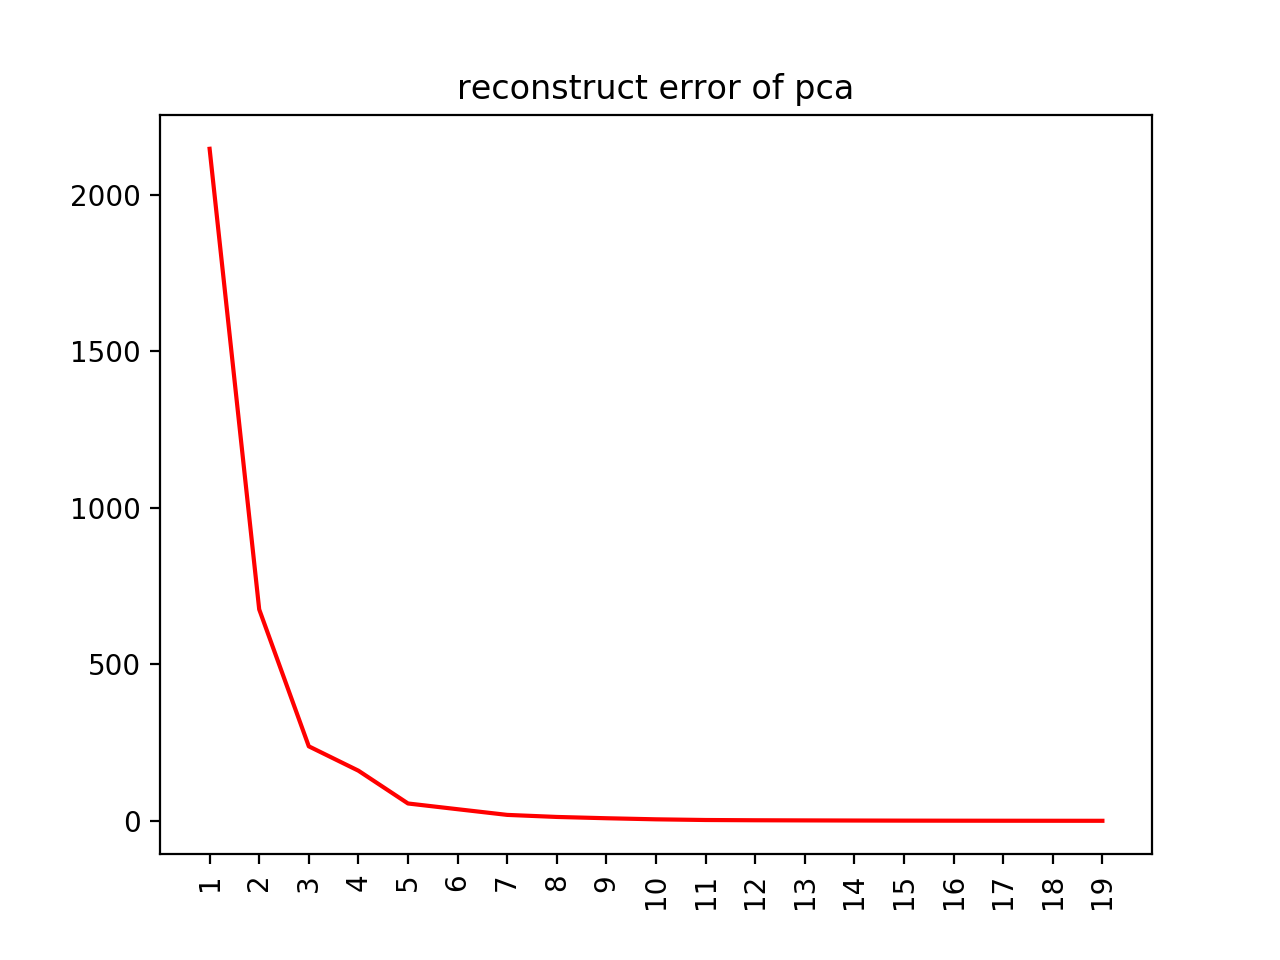
\includegraphics[width=.95\linewidth]{reconstruction_pca_dataset1}
     \end{minipage}\hfill
     \begin{minipage}{0.33\textwidth}
     \centering
     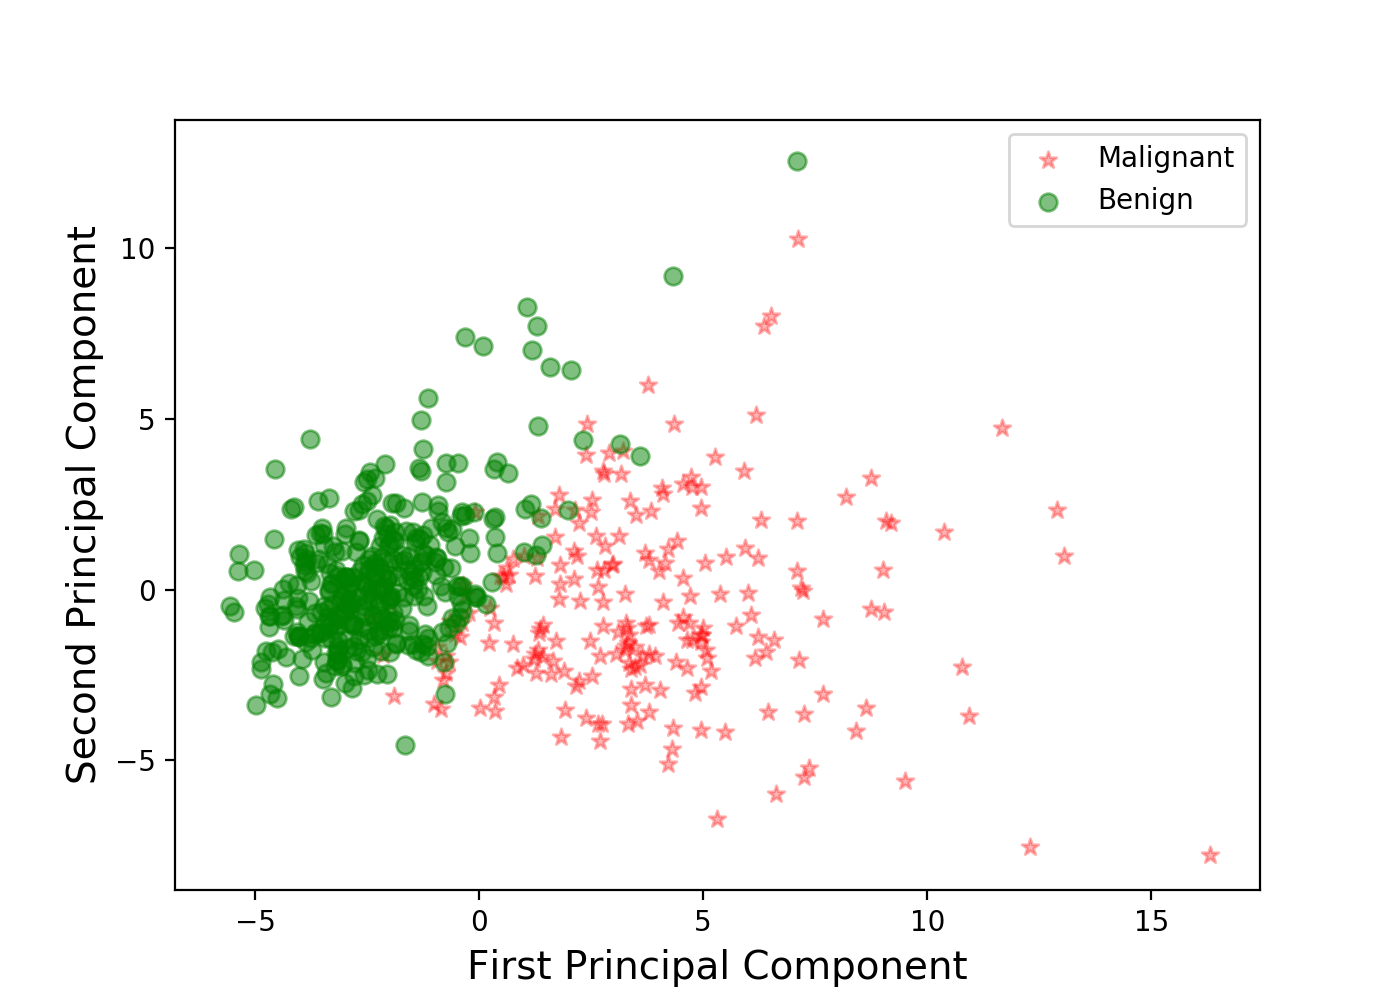
\includegraphics[width=.95\linewidth]{pca_d1_2}
   \end{minipage}\hfill
 \caption { Simulated Annealing Tuning}
\end{figure}
\textbf{ Kmeans After PCA }  The kmeans clustering ran on the modified data has the following changes as compared with the original data first the SA score is increased which means better and well defined clusters are formed. The SA score increased from 0.394 to 0.378 for the first dataset  which means that the cluster and the points are well separated now as is visible in the visualisation of the data and even a linear separator can also differentiate the data which means that the complexity of the classifier is reduced. The sample distribution with respect to clusters remain same. The number of clusters after the dimensionality reduction using PCA has not changed when we checked that using the elbow analysis as before only it was doing good. 
\begin{figure}[!htb]
\centering
   \begin{minipage}{0.48\textwidth}
     \centering
     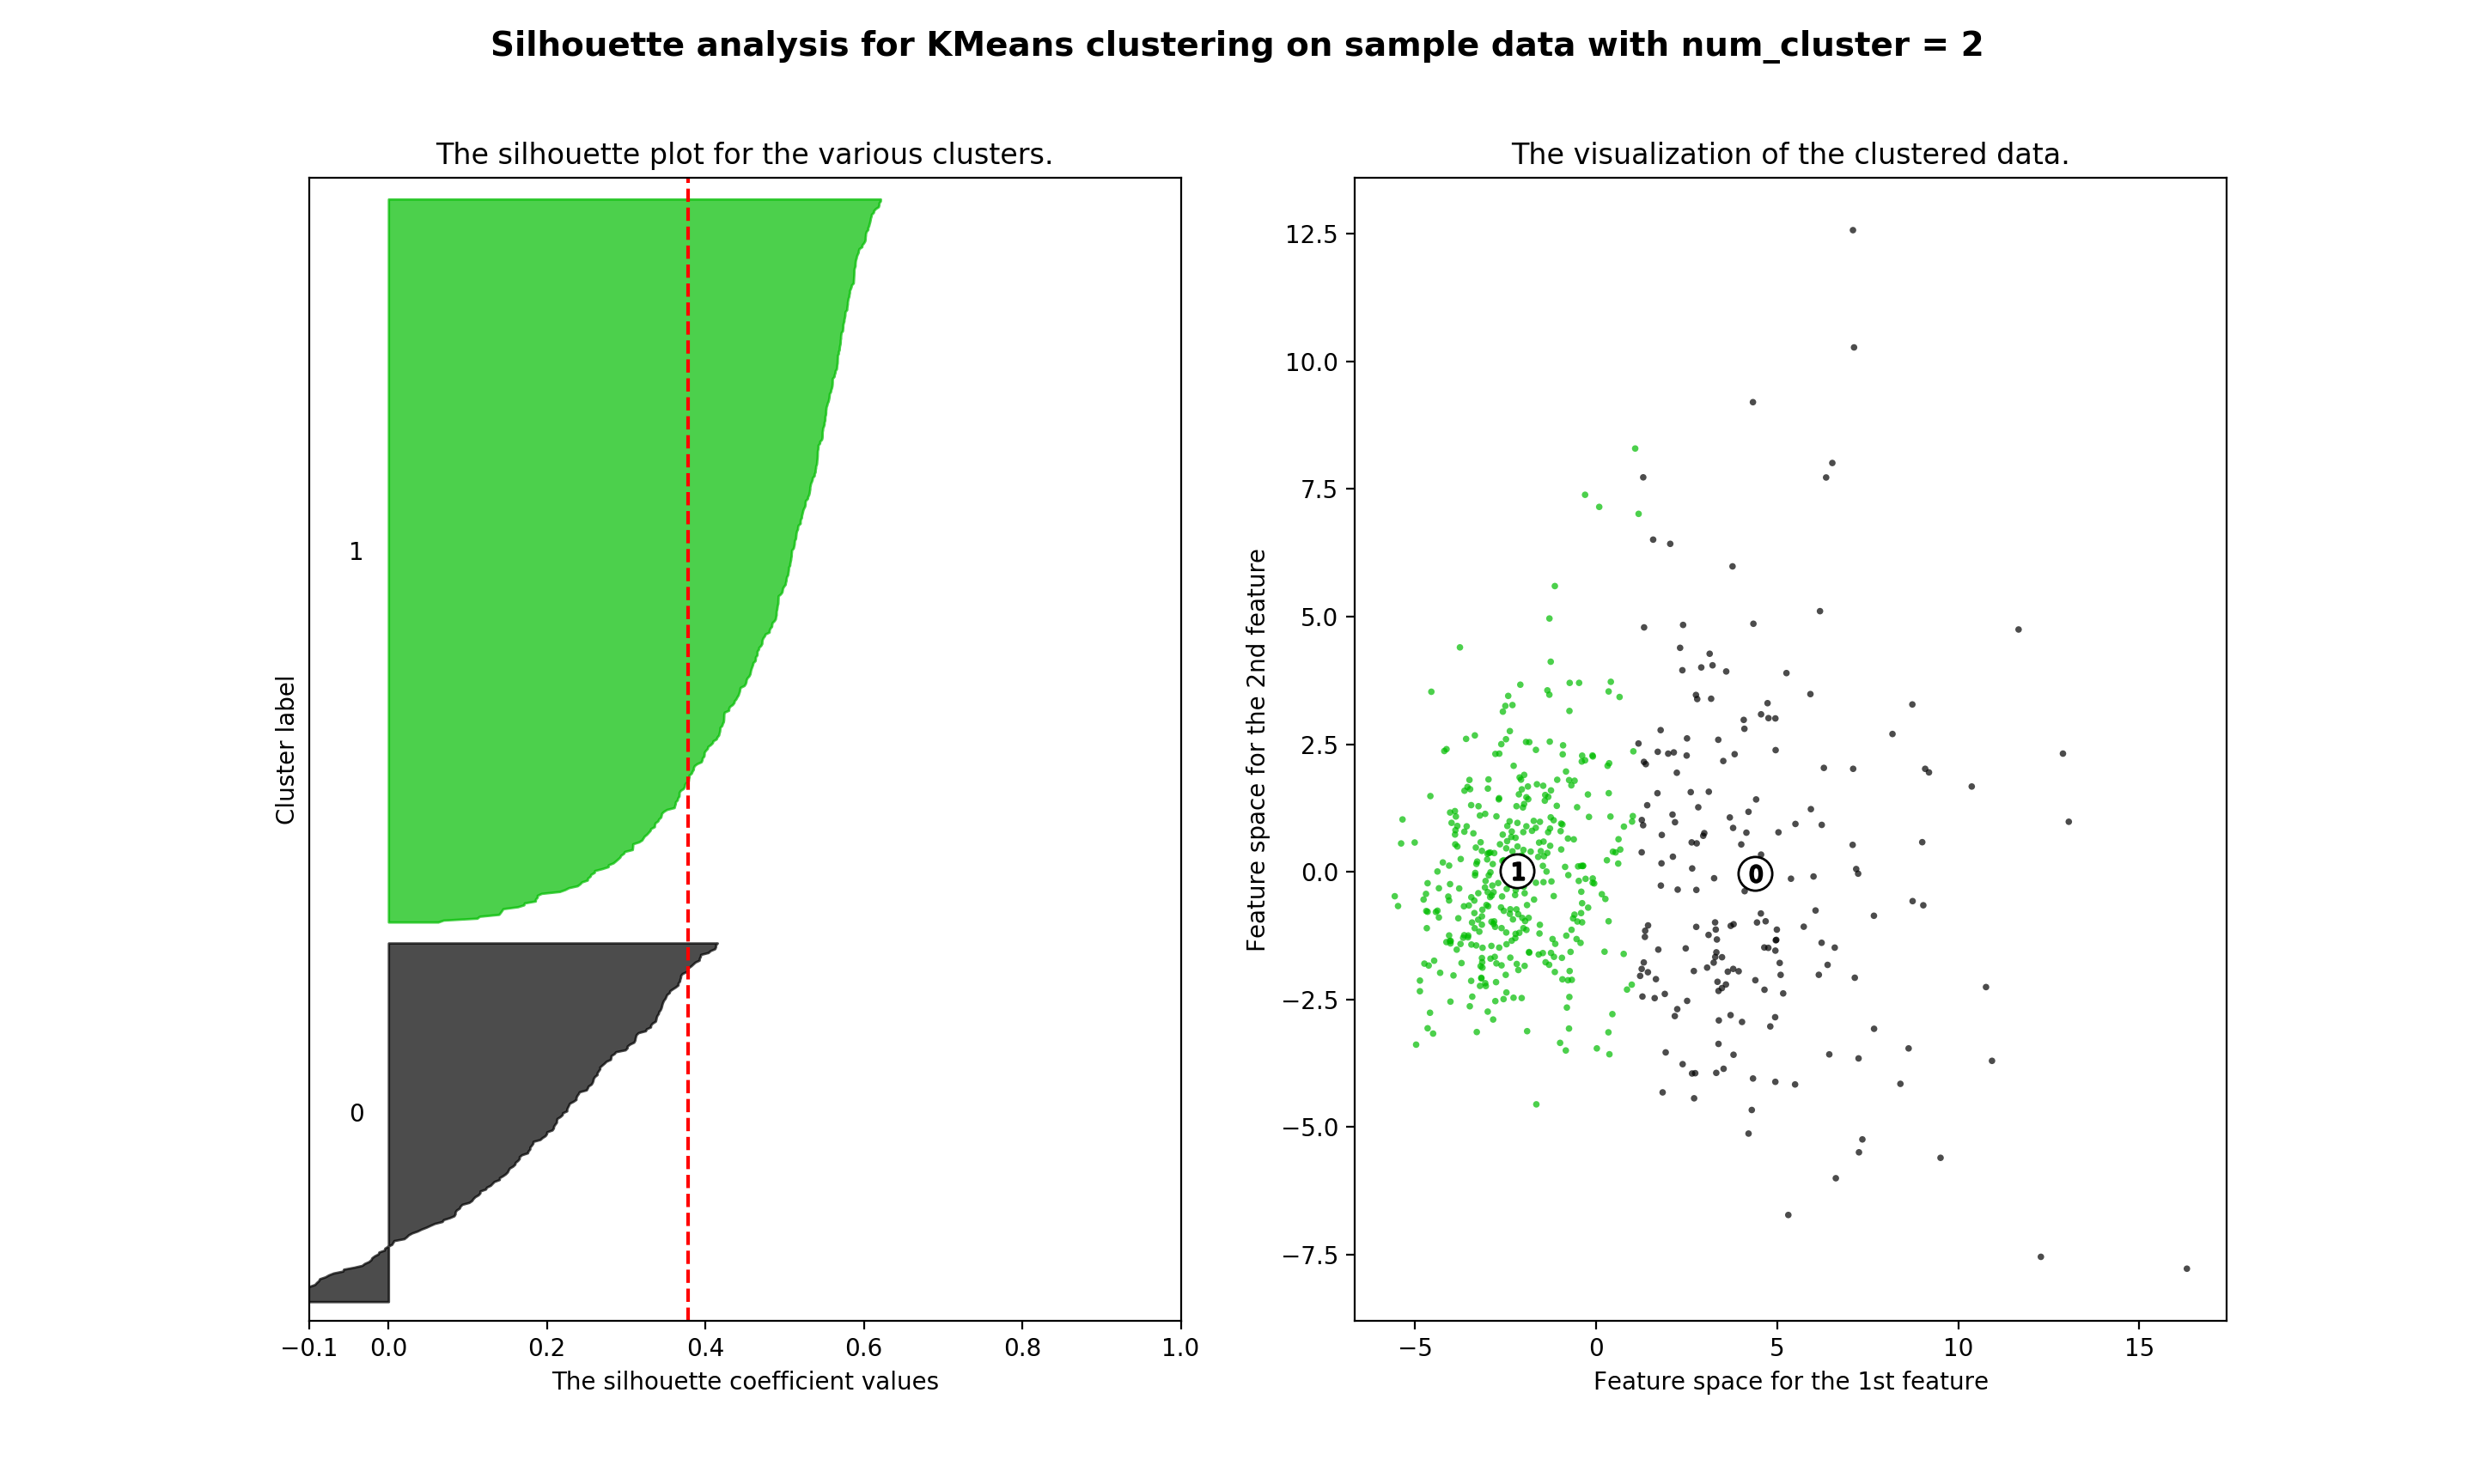
\includegraphics[width=.8\linewidth]{kmeans_d1_pca}
   \end{minipage}\hfill
    \begin{minipage}{0.48\textwidth}
     \centering
     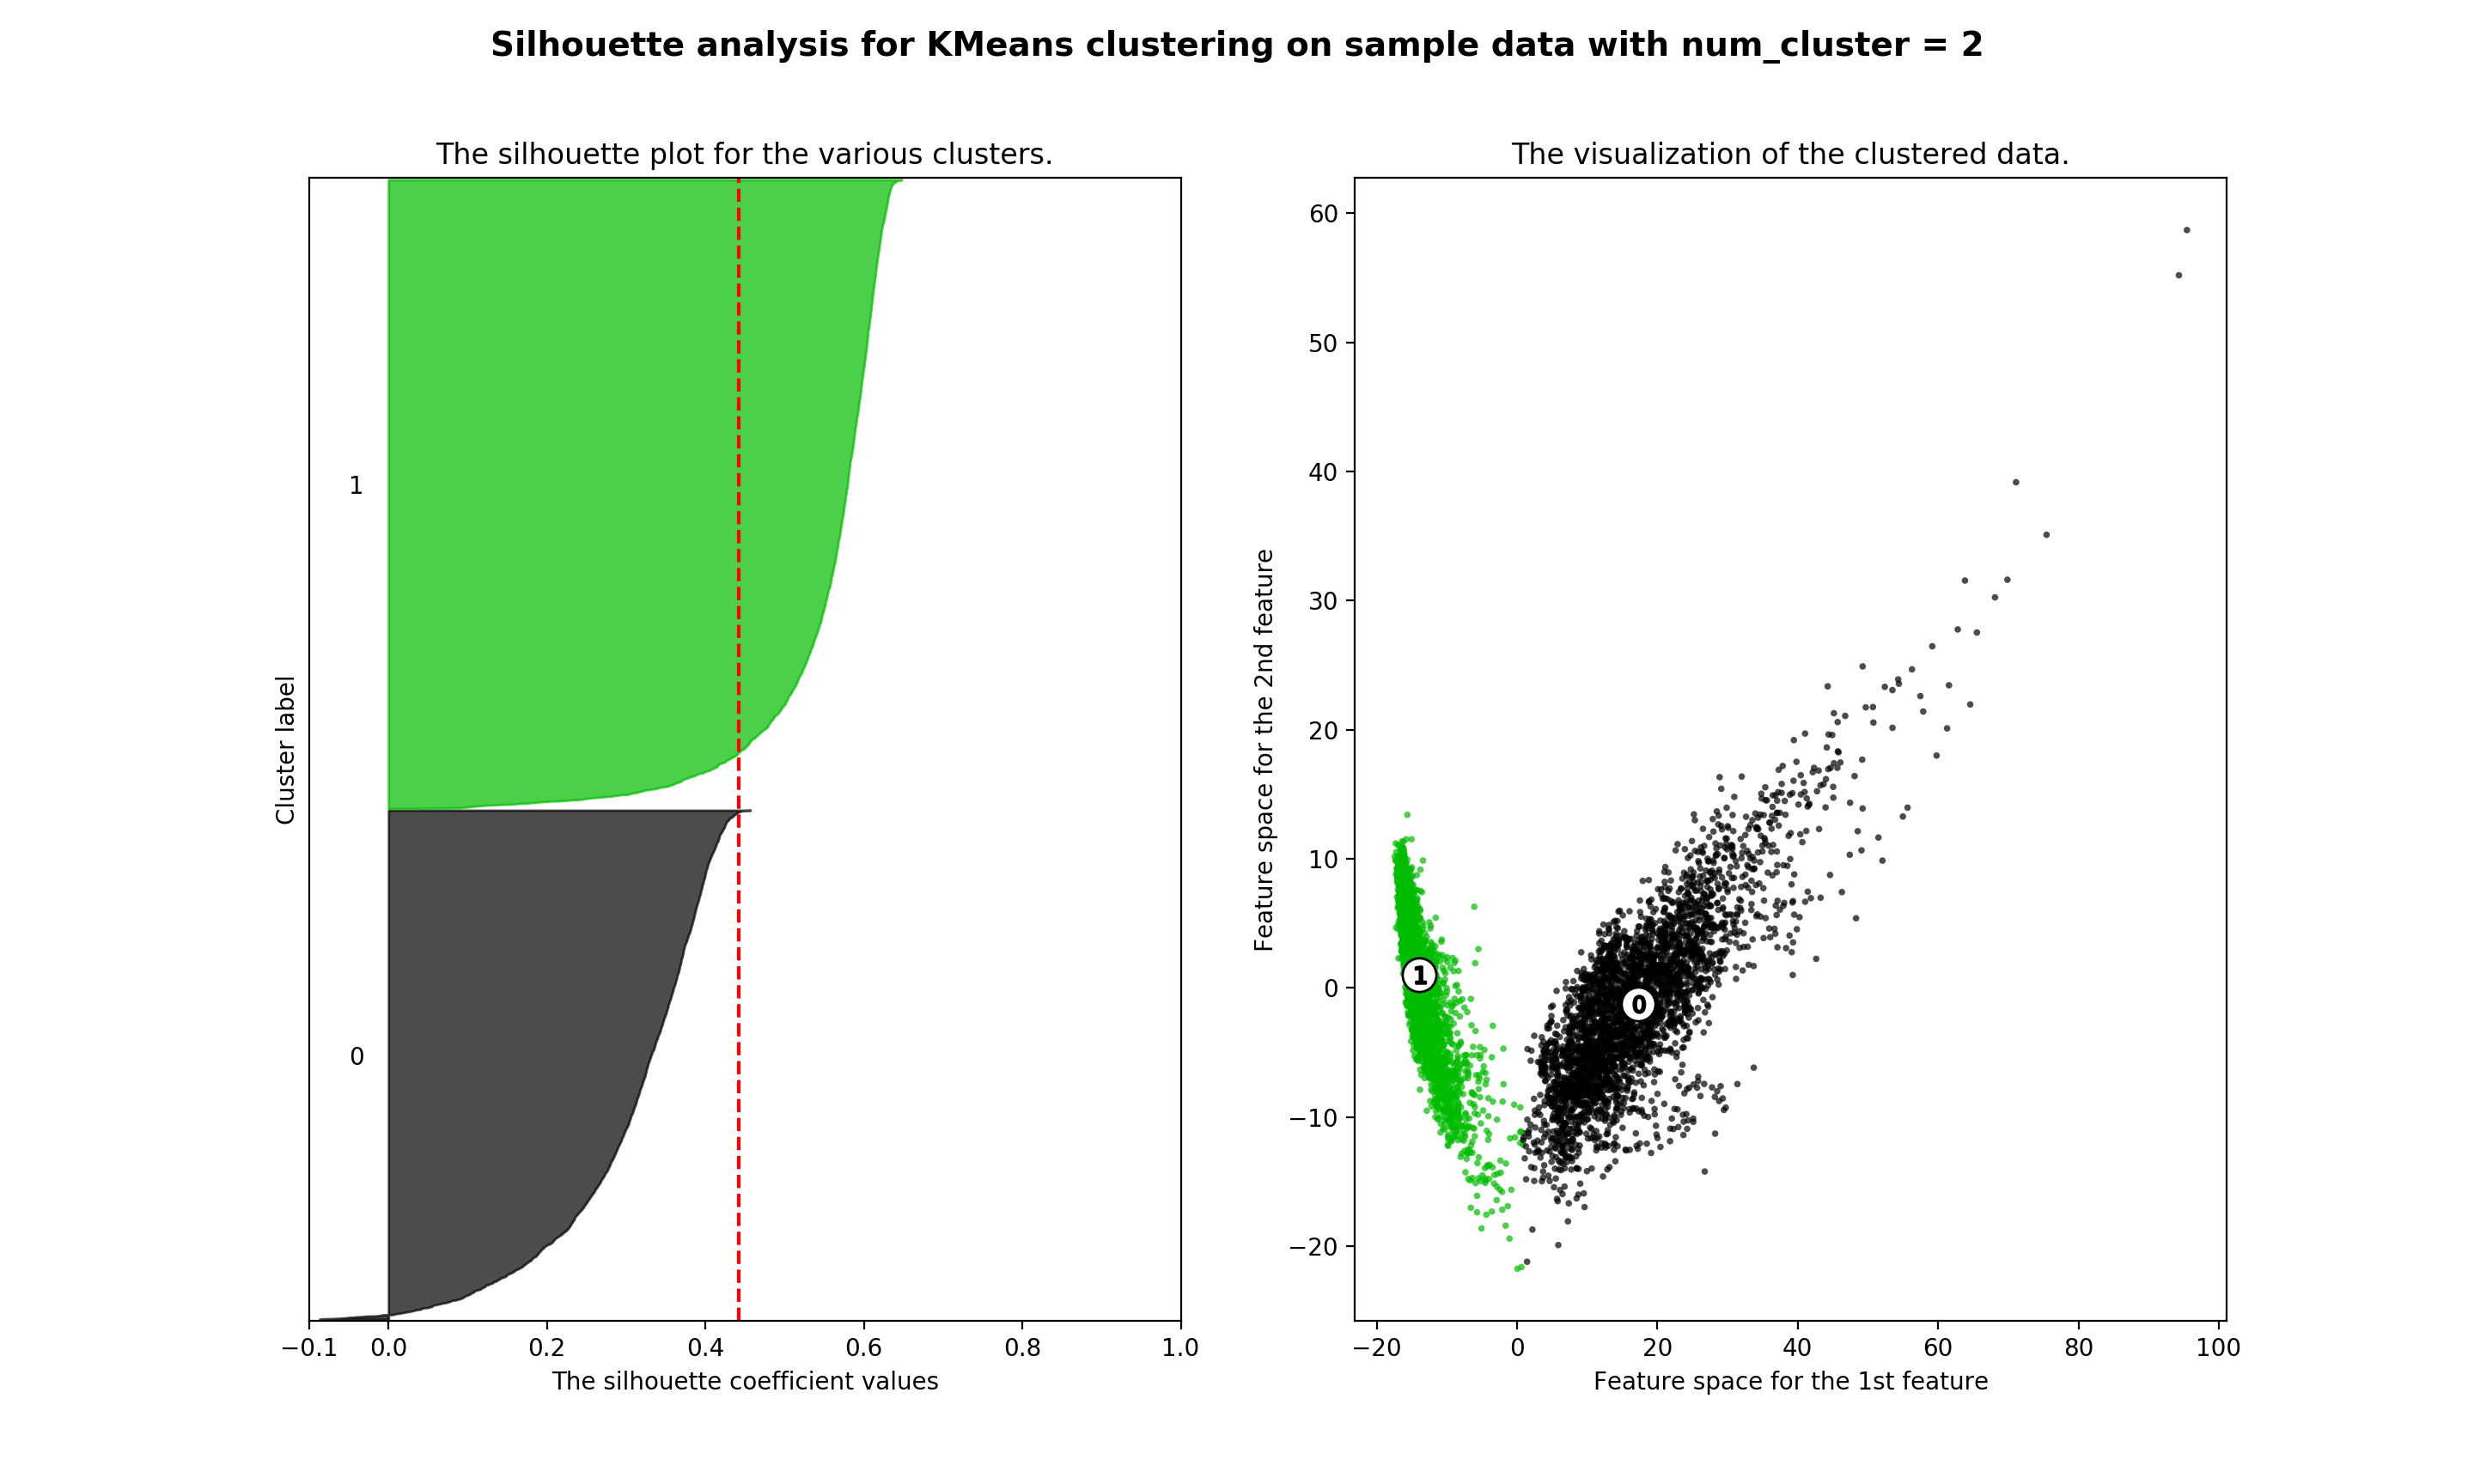
\includegraphics[width=.8\linewidth]{kmeans_d2_pca}
     
   \end{minipage}\hfill
   \caption { Four Peaks Description}
\end{figure}

\textbf{ Expectation Maximisation} The EM clustering algorithm performed after doing pca on the data set and choosing the appropriate number of components for the pca as shown perviously using the elbow analysis we performed the gmm ( gaussian mixture algorithm ) the hyperparamteres were selected using the same BIC criteria which showed that the number of components for the first dataset is 2 and covariance type as full and in the second dataset we got the number of components to be coincided with the labels which means EM was able to separate all the samples in the data set 2 after pca which the kmeans failed to do after pca also. Kmeans performs successfully on well separated data ,After we plotted the dataset variation in the 3d plot  we can see that the second dataset is not spherical in distribution due to which the kmeans fails to segregates the dataset 2 properly and this is where gmm covers this weakness using the covariance which describes the degree of freedom of each cluster. Kmeans expect the clusters to be spherical in nature.
\begin{figure}[!htb]
   \begin{minipage}{0.33\textwidth}
     \centering
     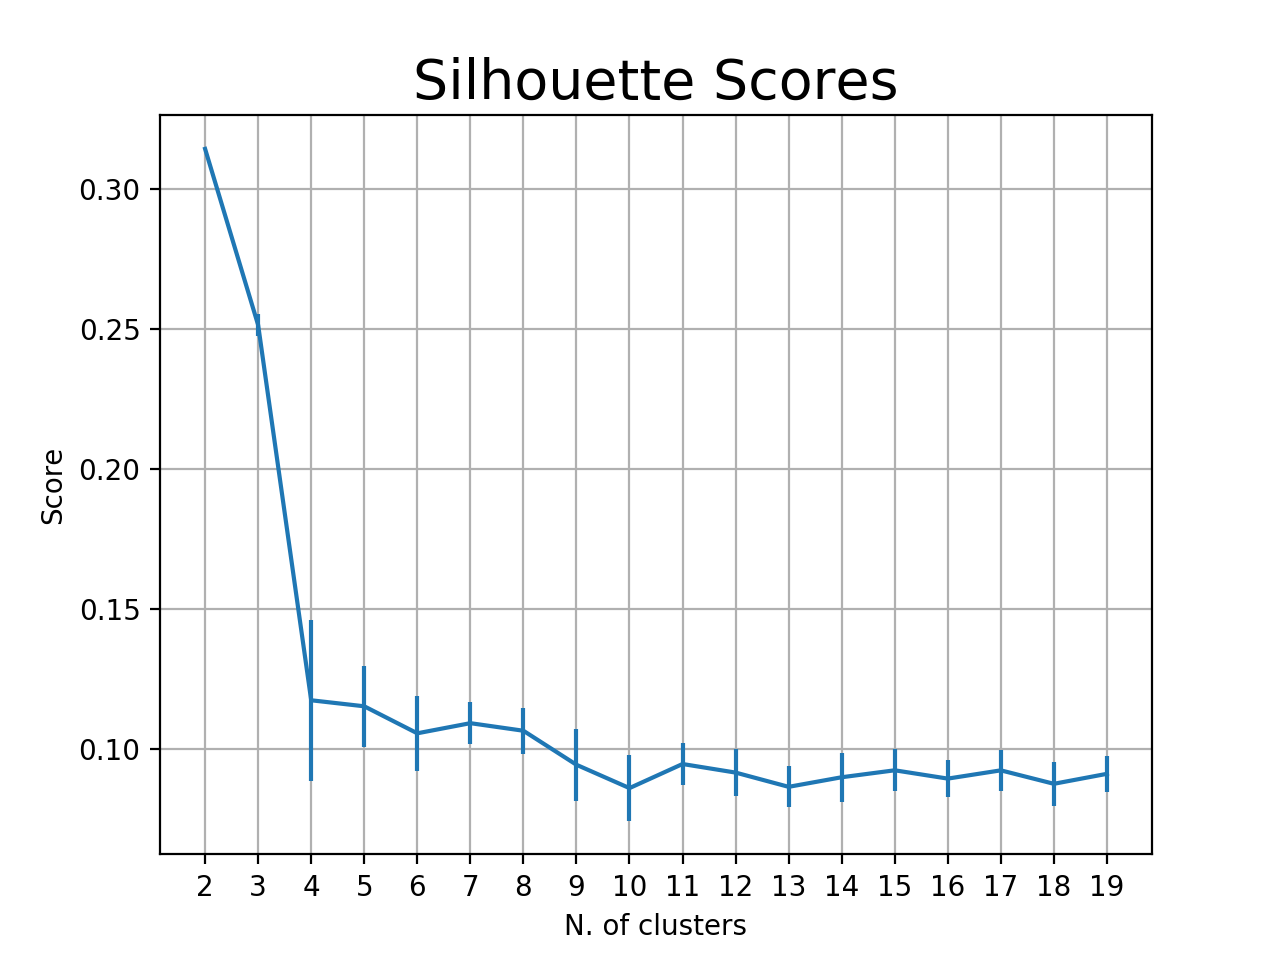
\includegraphics[width=.95\linewidth]{gmm_sil_1}
   \end{minipage}\hfill
    \begin{minipage}{0.33\textwidth}
     \centering
     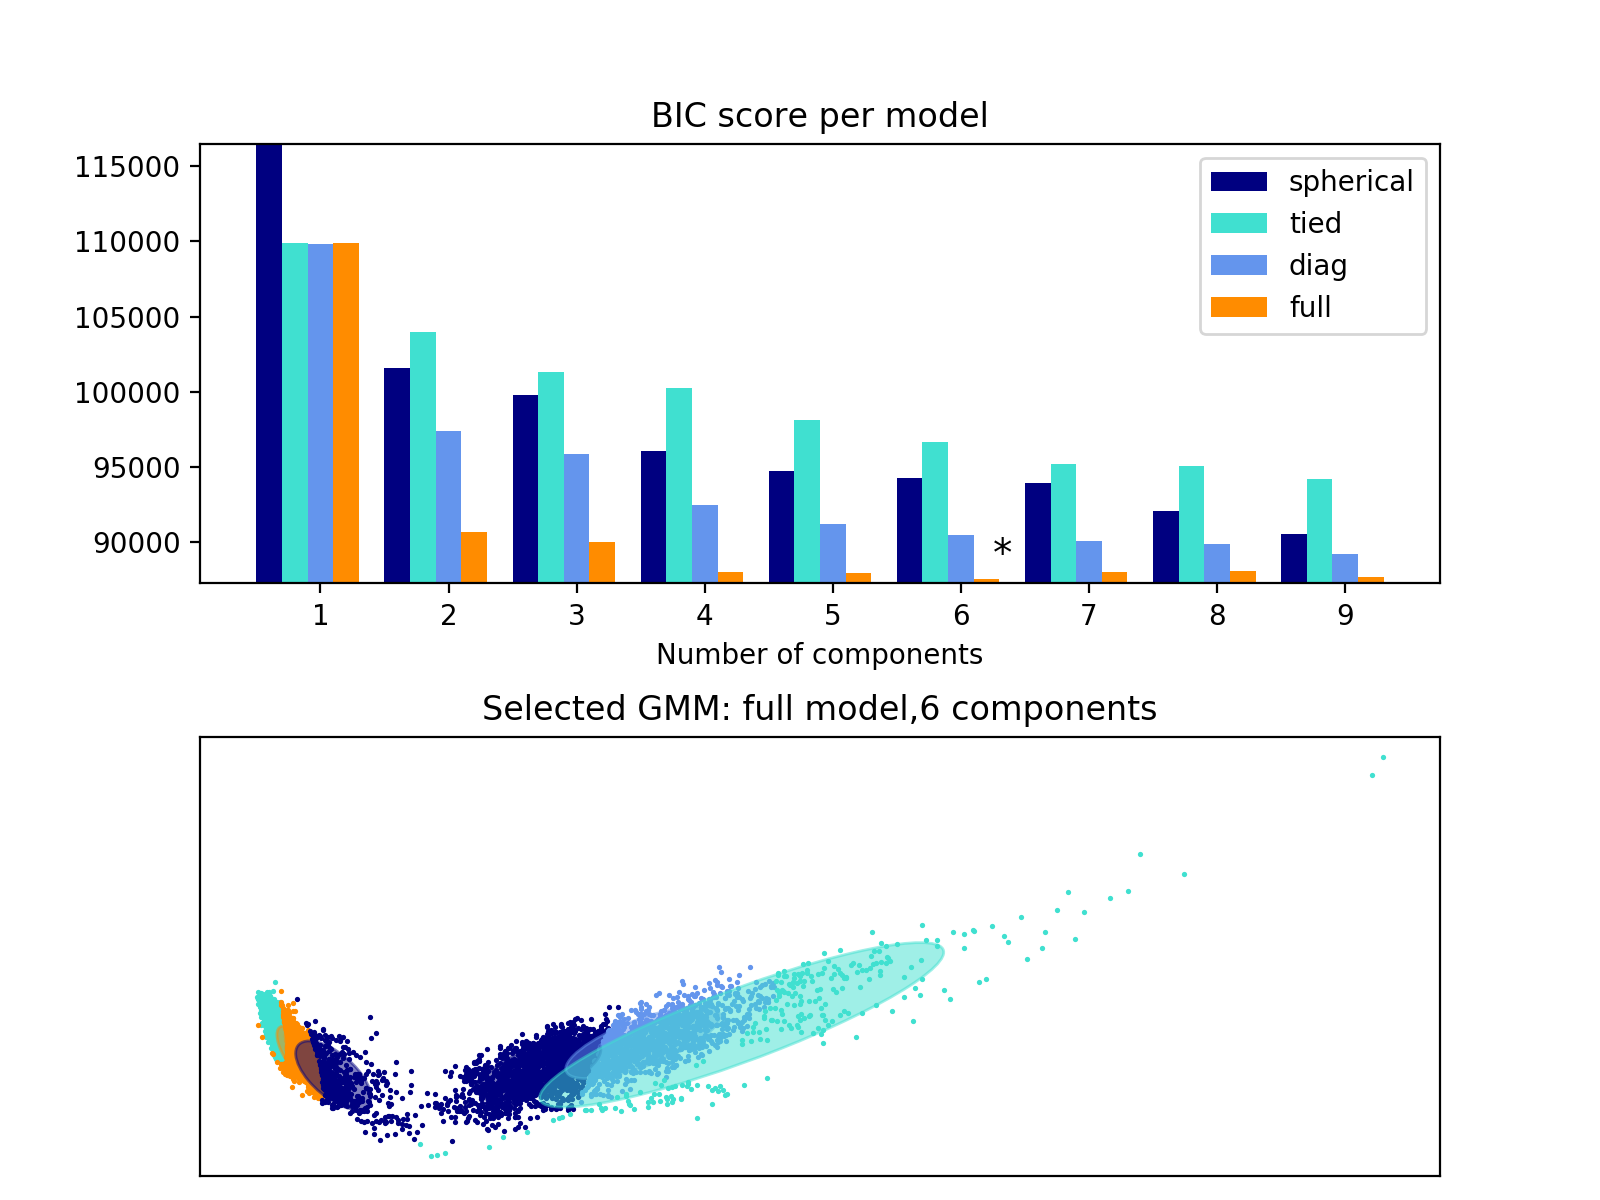
\includegraphics[width=.95\linewidth]{em_pca_d2}
     \end{minipage}\hfill
     \begin{minipage}{0.33\textwidth}
     \centering
     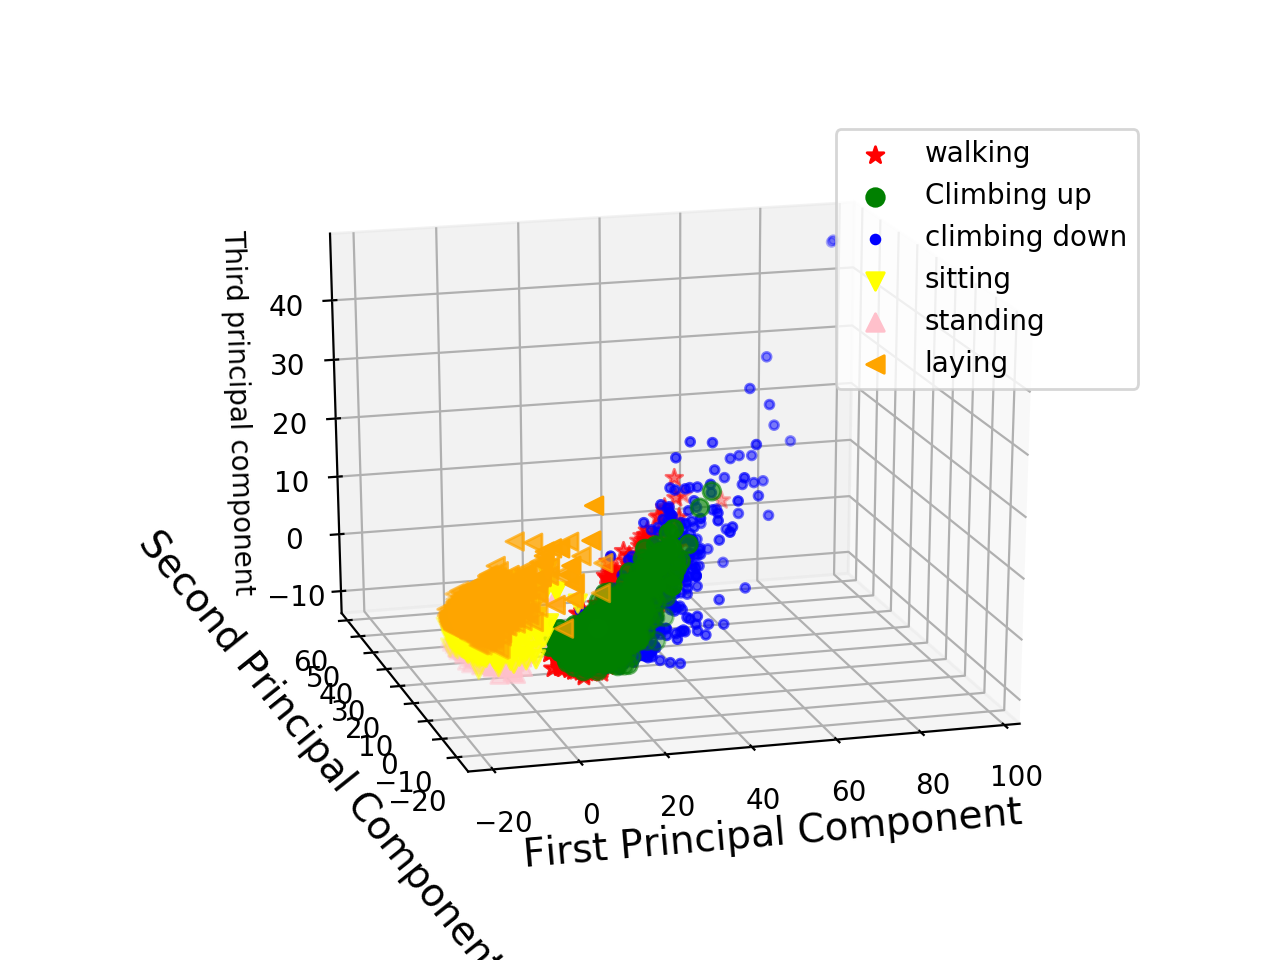
\includegraphics[width=.95\linewidth]{pca_data_set_2}
   \end{minipage}\hfill
 \caption { Simulated Annealing Tuning}
\end{figure}

\textbf{ICA} Independent component analysis attempts to decompose a multivariate signal into independent non-Gaussian signals. Independent Component Analysis focuses on restructuring the input data by increasing the separation between each of the components from one another by finding basis vectors that are independent components of the original data, implemented using the FastICA algorithm in sklearn. The number of independent components to select is done using the kurtosis analysis and the reconstruction error using ICA. The maximum kurtosis value for the first dataset occurs at component 5 , the kurtosis value which measures the extreme values in either tails with respect to the normal distribution large kurtosis exhibit tail data exceeding the tails of the normal distribution. After applying ICA we can see that some of the resulting features exhibited high non gaussian nature depicted in the kurtosis graph such as IC5 , IC4, IC6 etc. 

\textbf{Kmeans Clustering}The kurtosis values associated with the components were sorted and then were used for the clustering starting with IC5 which has the highest value , the parameters for the clustering were the SA analysis , accuracy of the cluster and the elbow analysis using all the parameters the components were selected to be 2. The kmeans clusters came out to be 2 where the accuracy was highest and the SA score was also the maximum we can see in the graph below  plots of the accuracy , SA values. The data visualisation with the cluster equal to 2 is shown.
\begin{figure}[!htb]
   \begin{minipage}{0.33\textwidth}
     \centering
     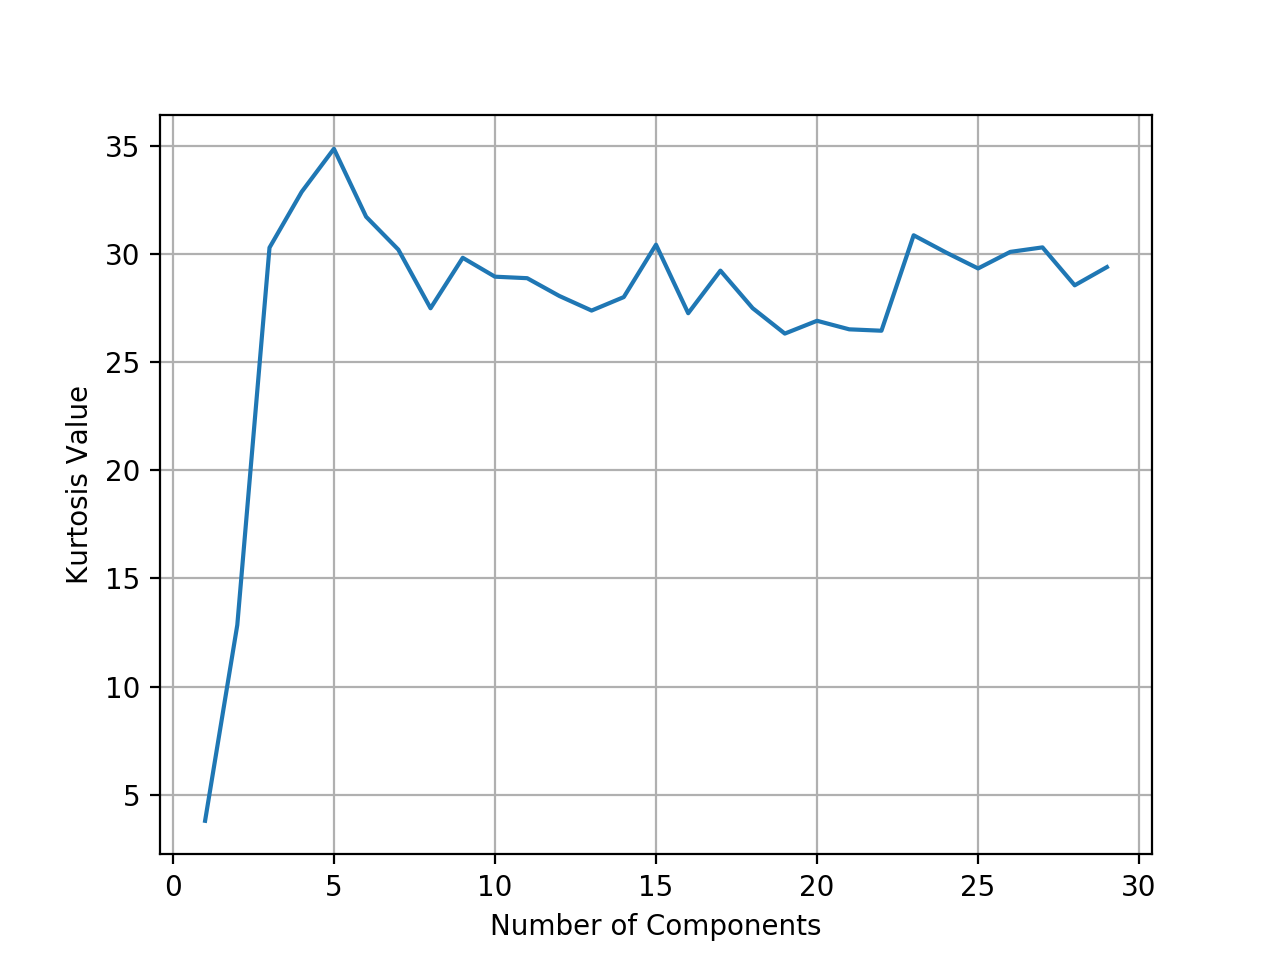
\includegraphics[width=.95\linewidth]{ica_dataset1}
   \end{minipage}\hfill
    \begin{minipage}{0.33\textwidth}
     \centering
     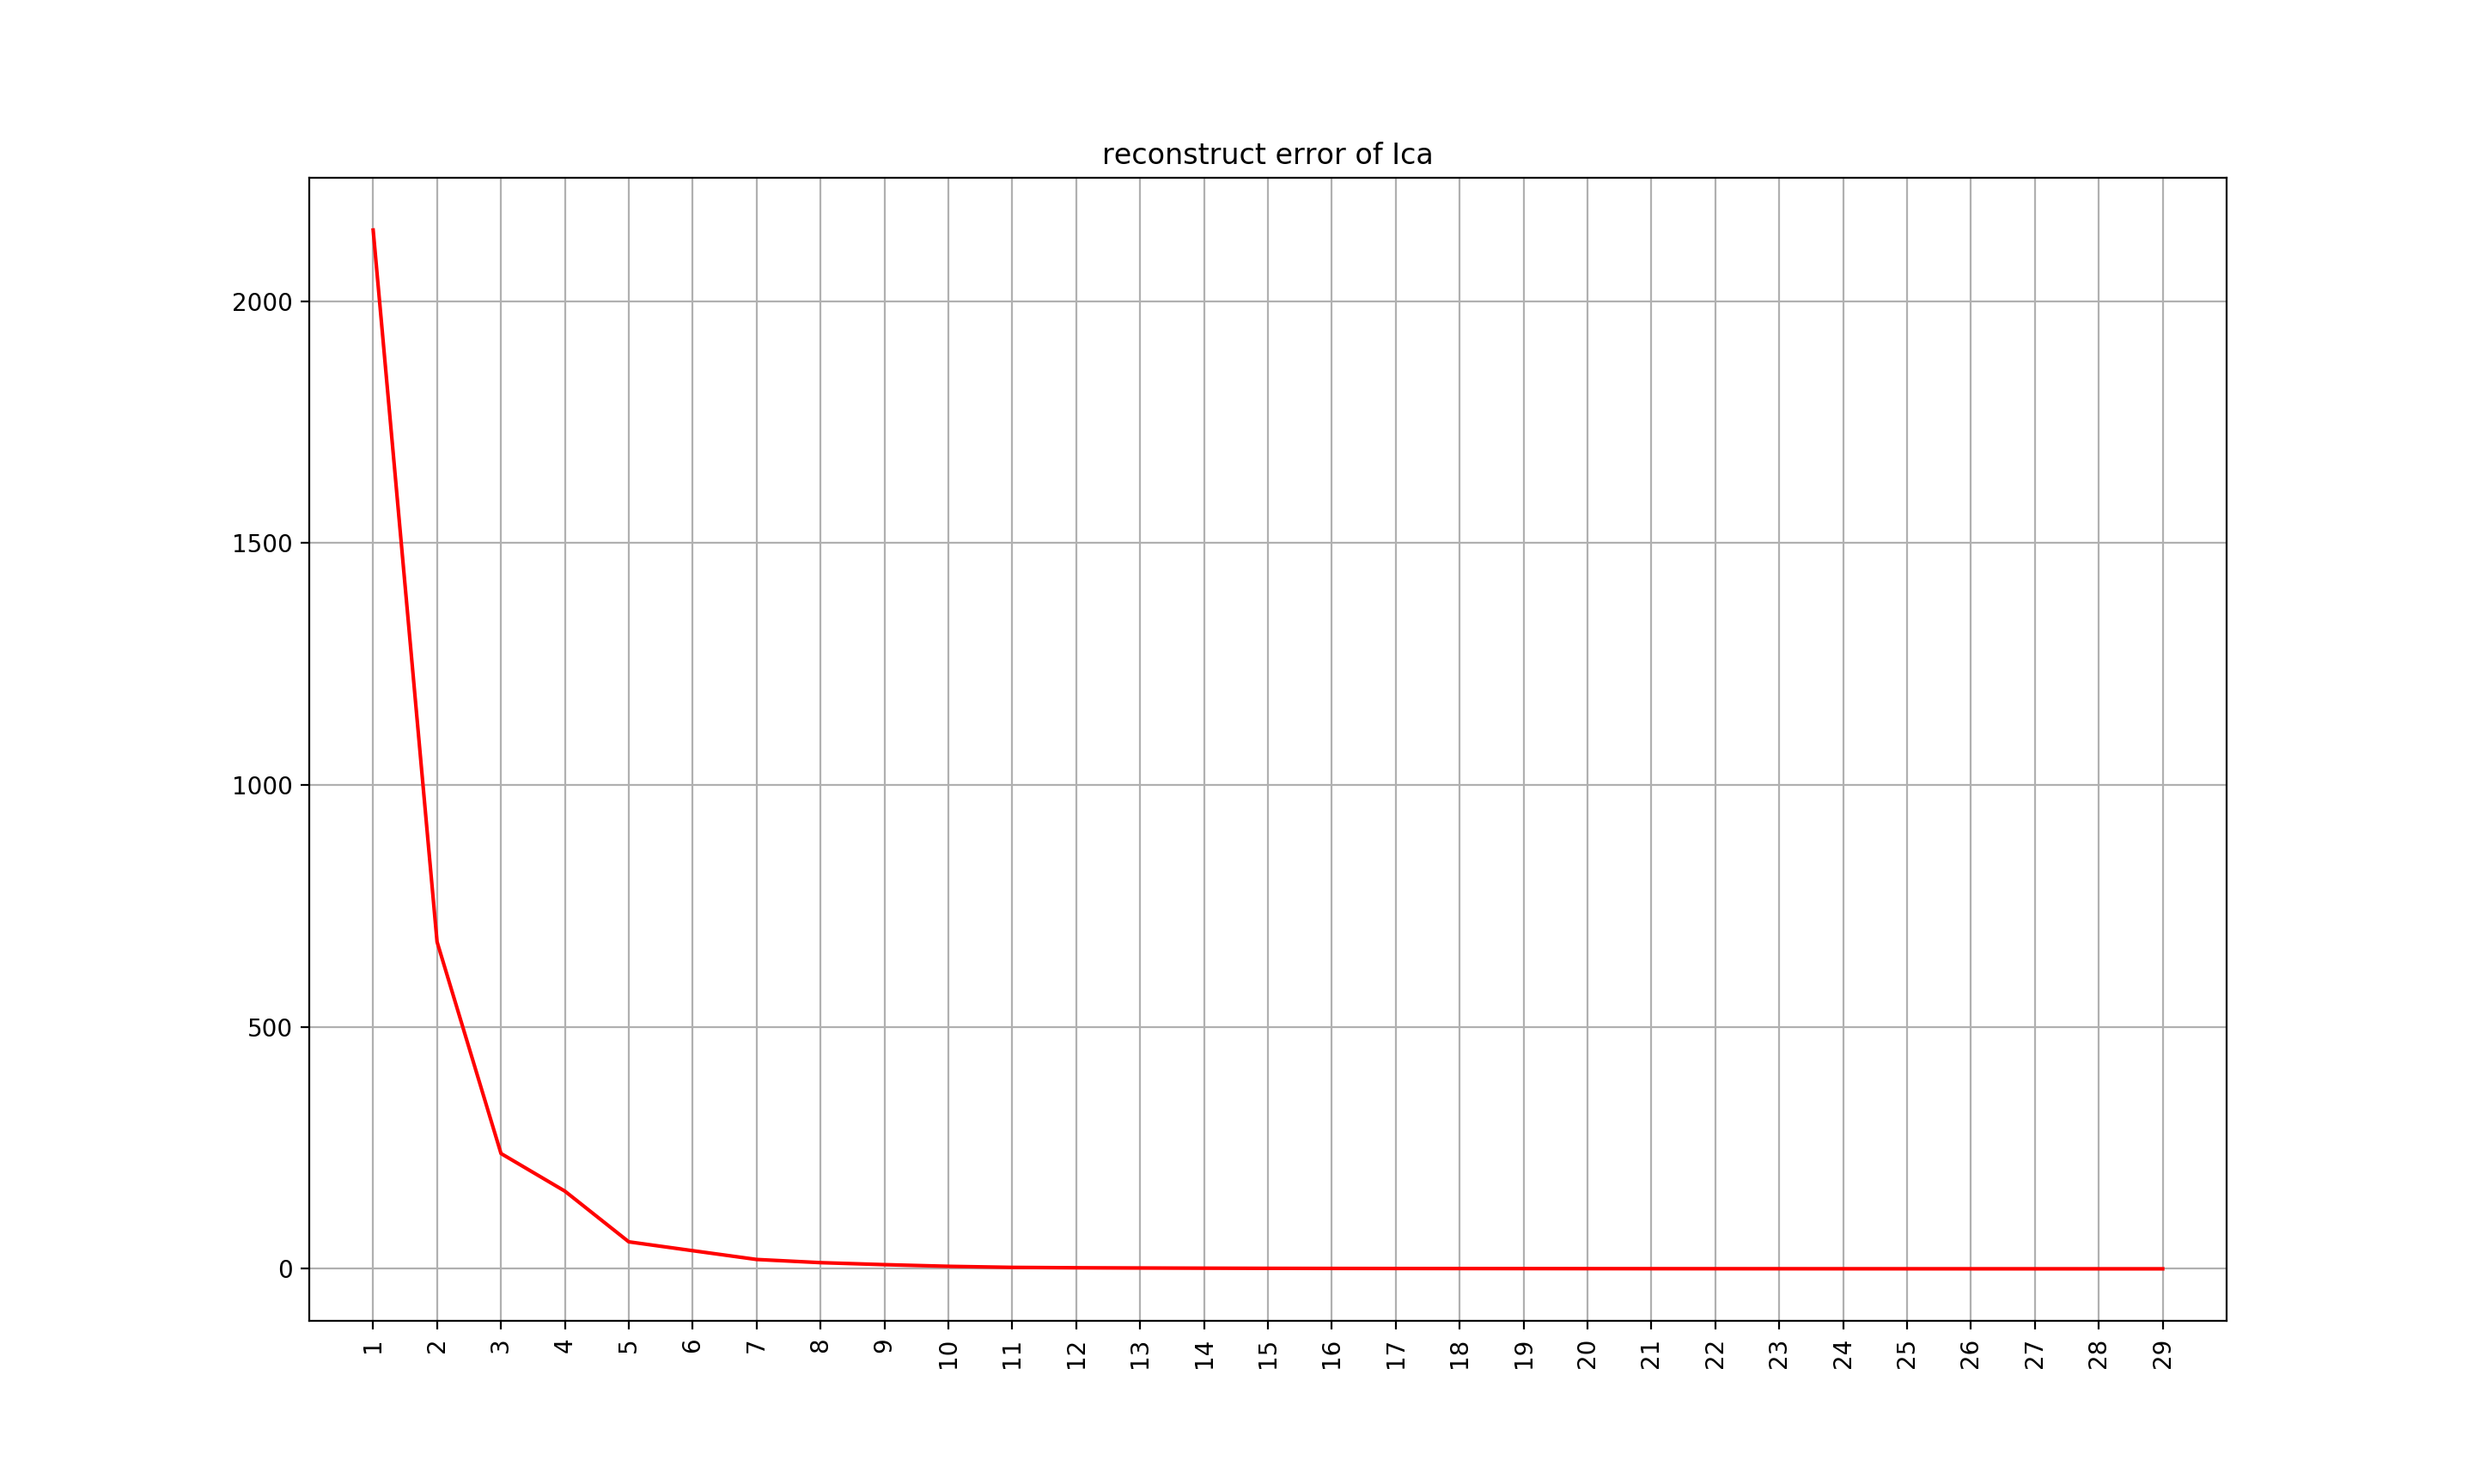
\includegraphics[width=.95\linewidth]{recons_ica_dataset1}
     \end{minipage}\hfill
     \begin{minipage}{0.33\textwidth}
     \centering
     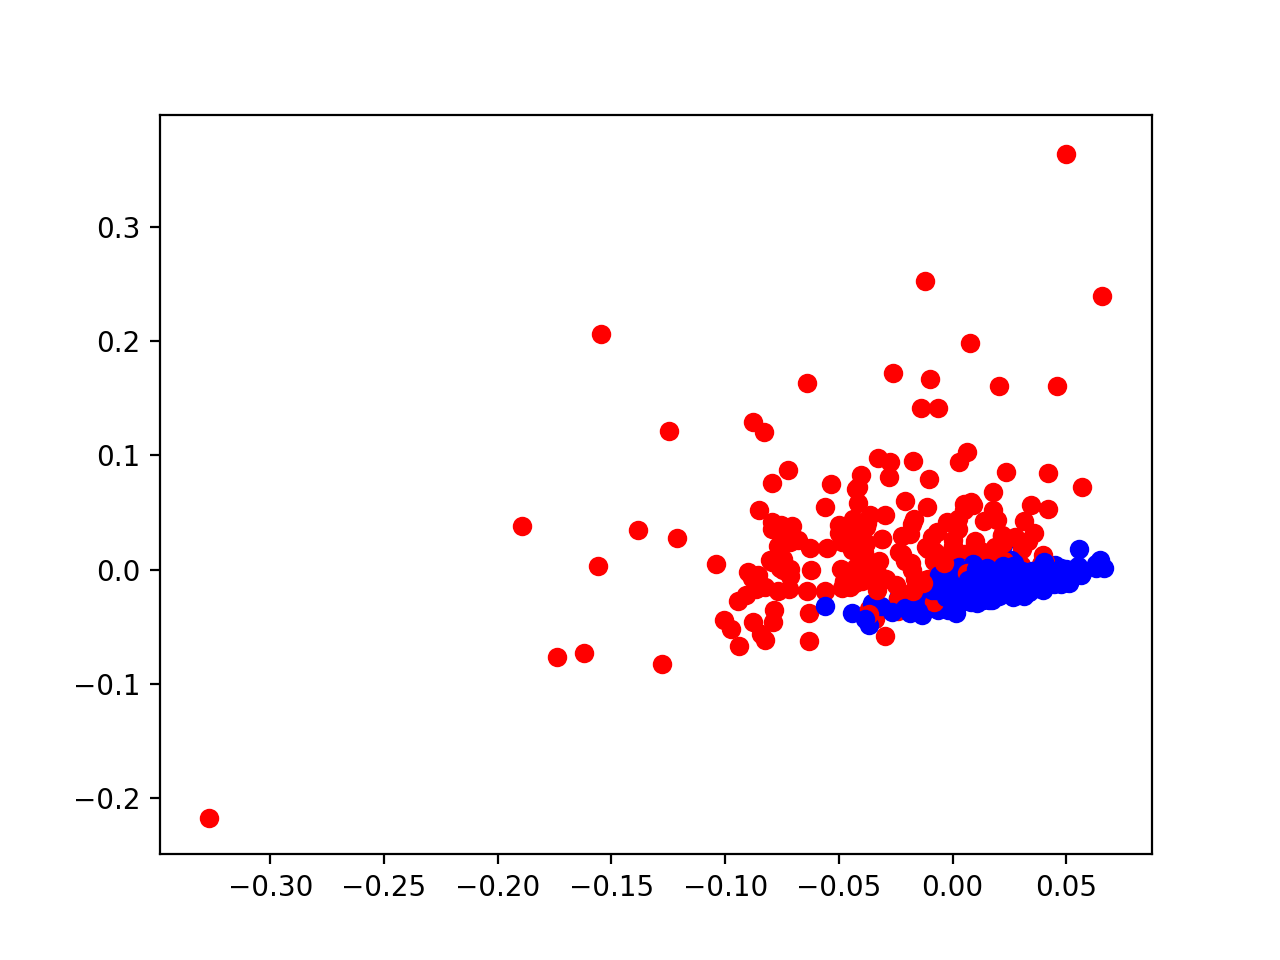
\includegraphics[width=.95\linewidth]{ica_d1_visuak}
   \end{minipage}\hfill
 \caption { Simulated Annealing Tuning}
\end{figure}

\textbf{EM analysis } For the EM the number of components to be found were evaluated using the SA analysis which were found to be 2 which coincided with the Kmeans and the number of labels also. The covariance type was found to be full. The graph is plotted which shows the SA score with the number of clusters. one thing which was noted clustering after the dimensionality reduction was the reduction in the number of iterations to converge for the from 15 to 4.\newline
\begin{figure}[!htb]
   \begin{minipage}{0.33\textwidth}
     \centering
     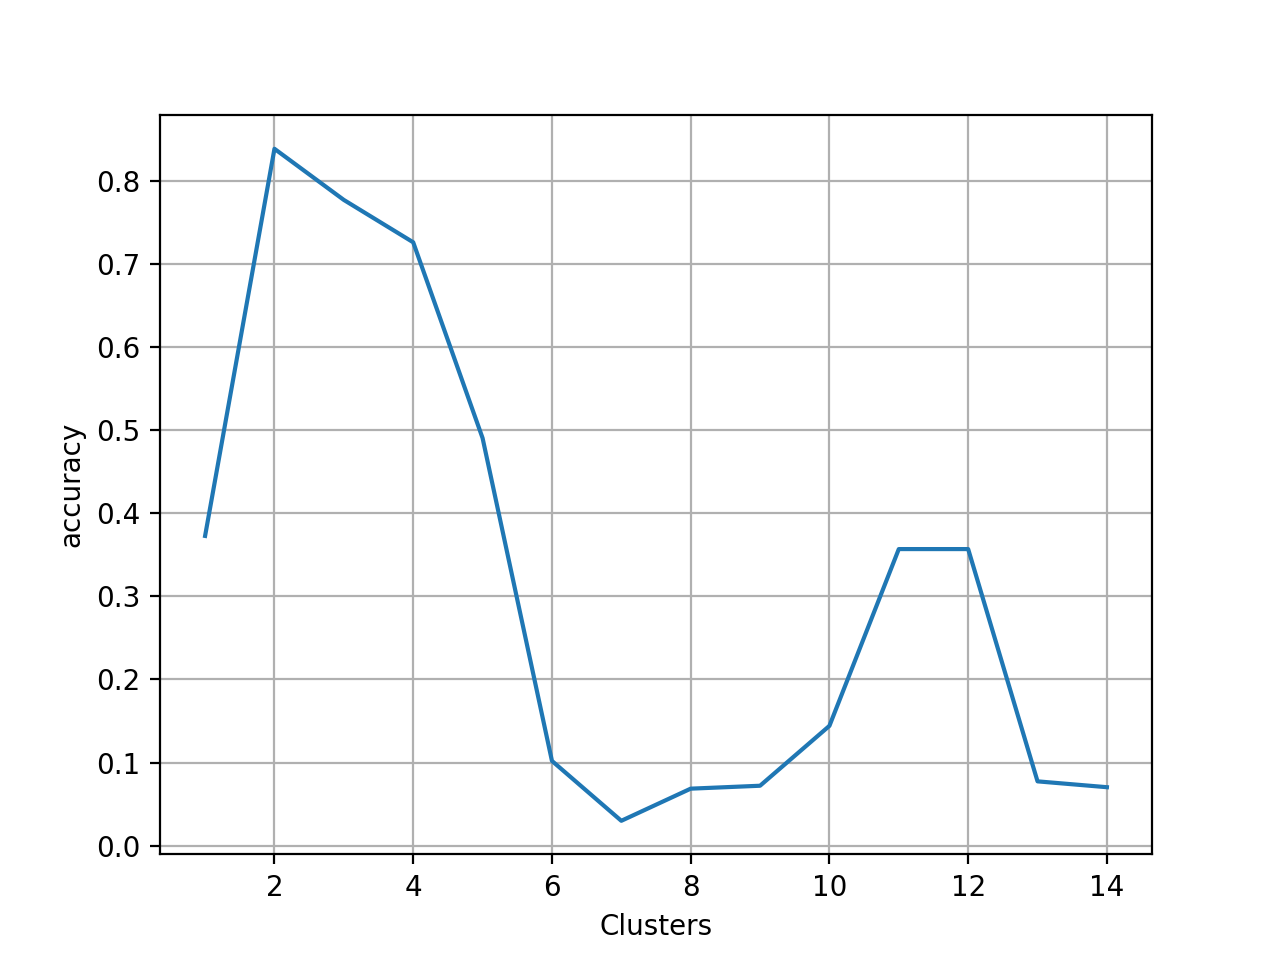
\includegraphics[width=.95\linewidth]{kmeans_ica_dataset1_accuracy}
   \end{minipage}\hfill
    \begin{minipage}{0.33\textwidth}
     \centering
     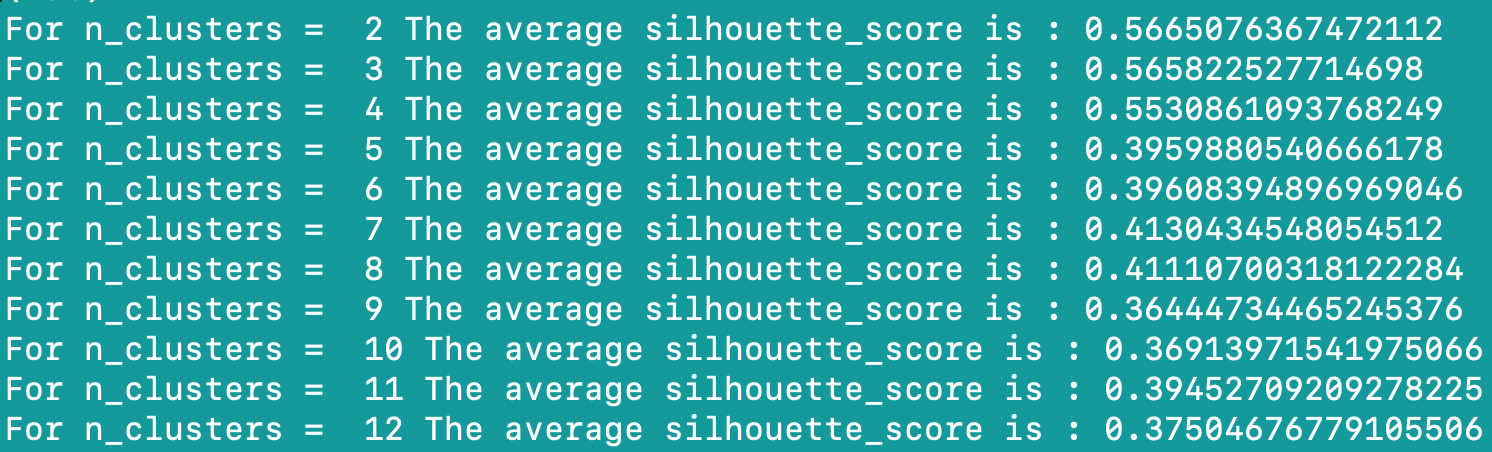
\includegraphics[width=.95\linewidth]{kmeans_ica_dataset1_sil}
     \end{minipage}\hfill
     \begin{minipage}{0.33\textwidth}
     \centering
     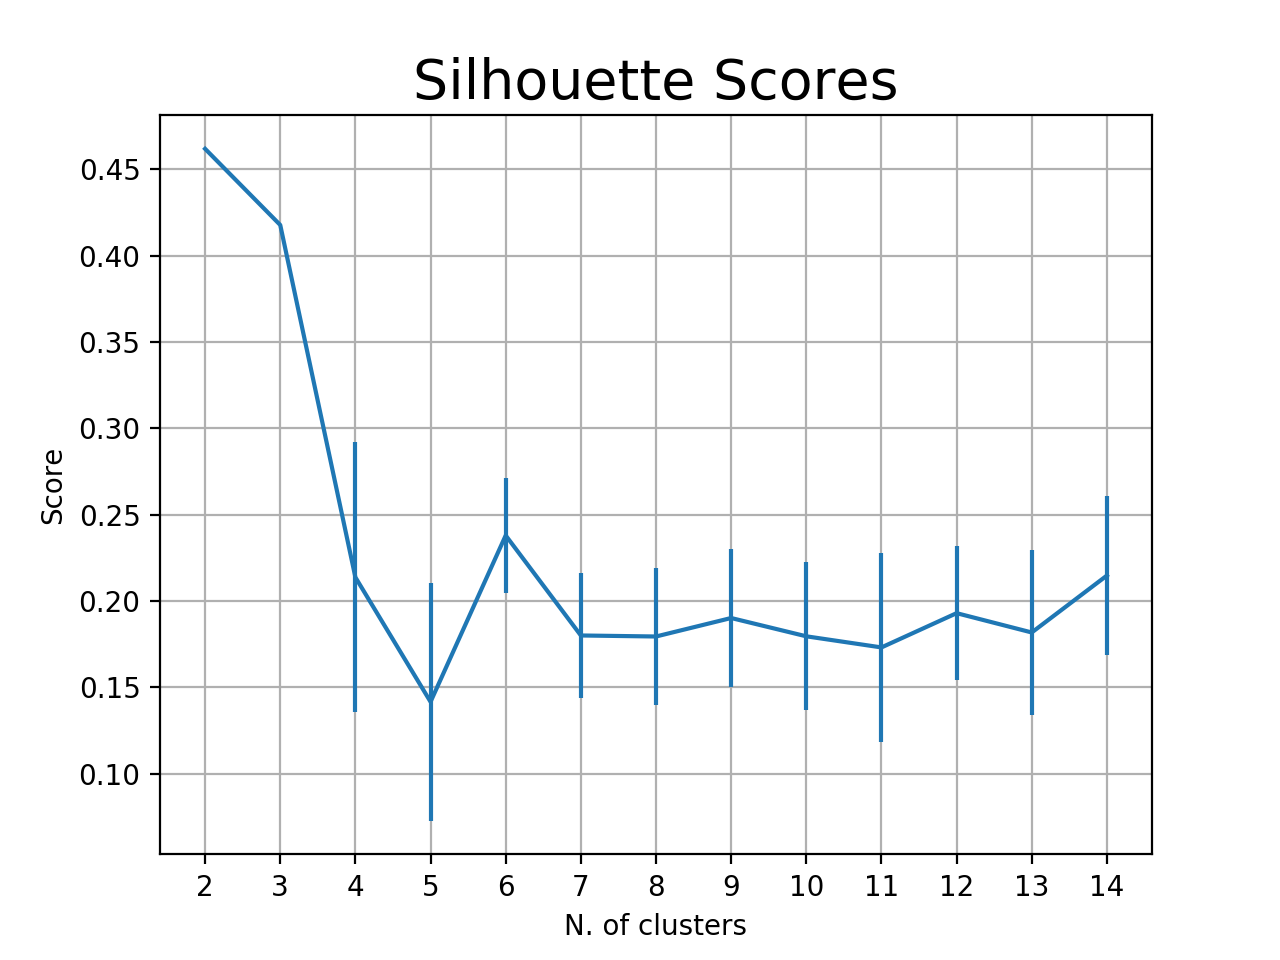
\includegraphics[width=.95\linewidth]{em_ica_dataset1_sil}
   \end{minipage}\hfill
 \caption { Simulated Annealing Tuning}
\end{figure}
\textbf{ Data set 2 ICA} For this dataset the IC's were expected to be more as the number of features were more as compared with the cancer dataset and we can see that the max kurtosis value is 40, this also means that the features are highly non gaussian which is good as this is what the ICA is intended to do.The components value is sorted and tested according to the 

\begin{figure}[!htb]
   \begin{minipage}{0.33\textwidth}
     \centering
     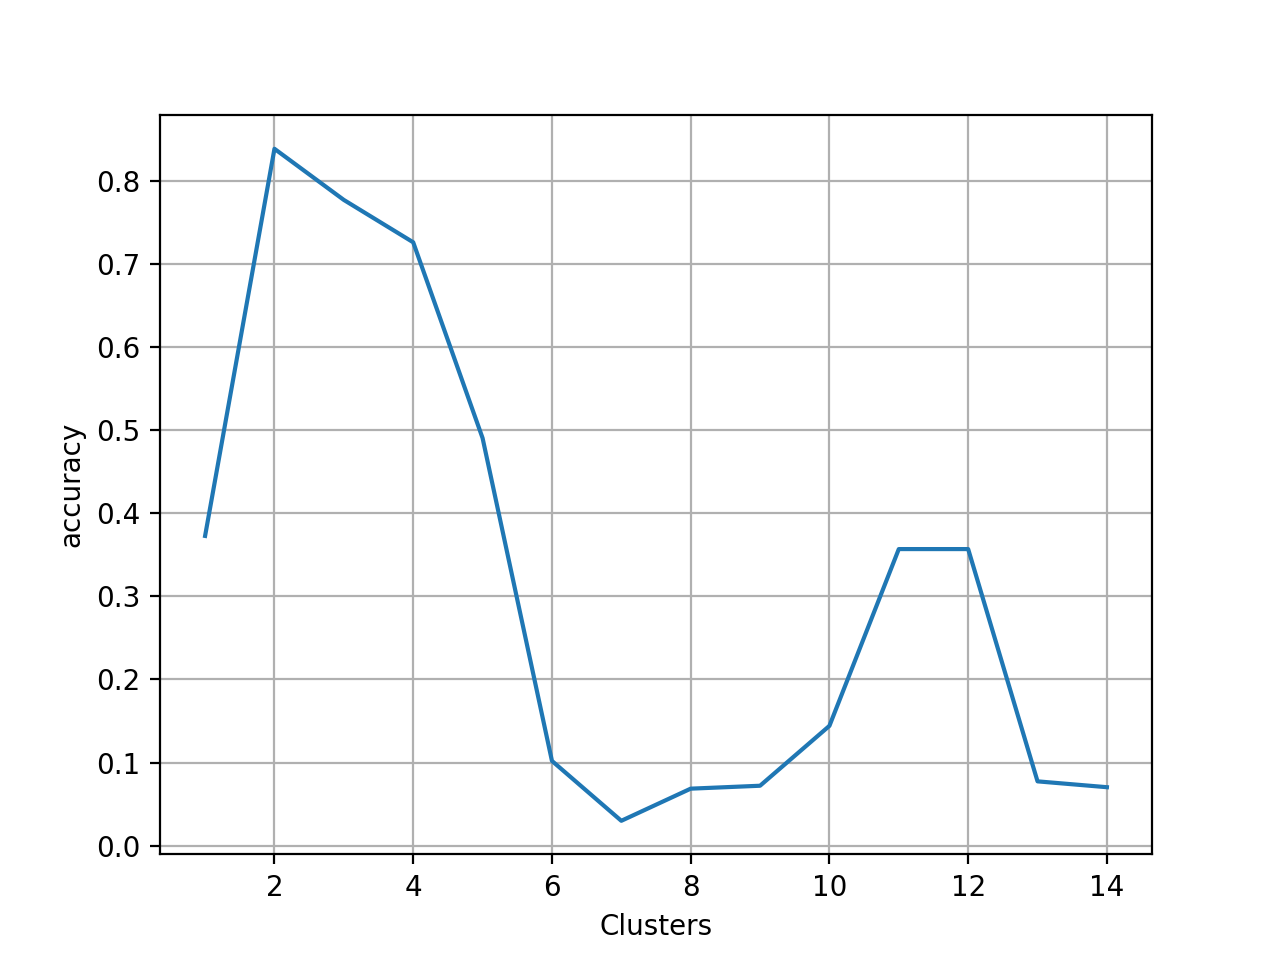
\includegraphics[width=.95\linewidth]{kmeans_ica_dataset1_accuracy}
   \end{minipage}\hfill
    \begin{minipage}{0.33\textwidth}
     \centering
     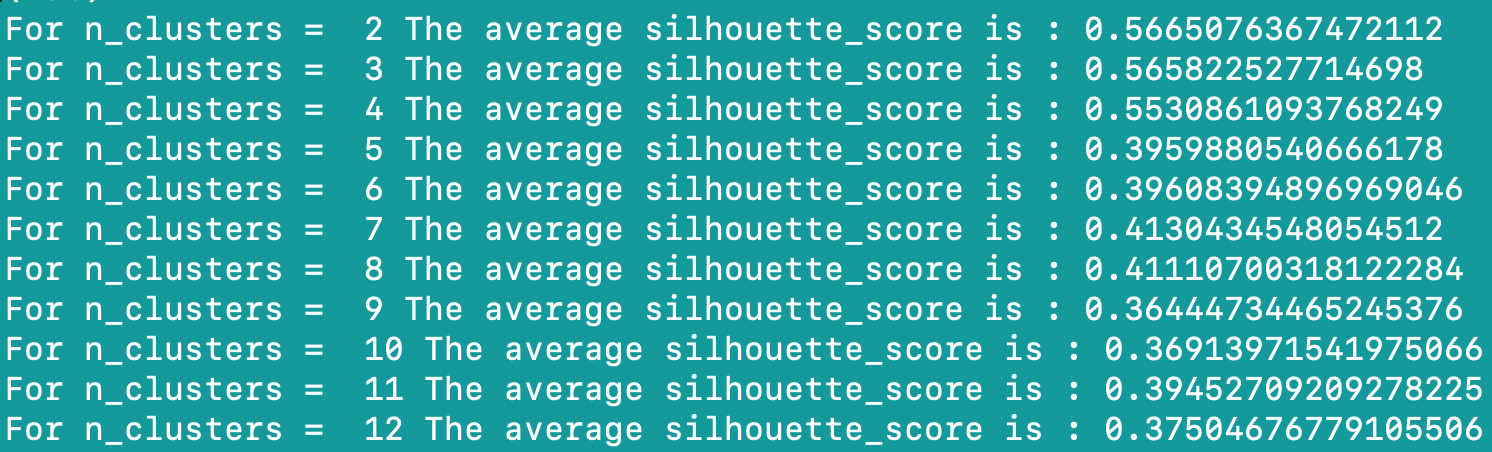
\includegraphics[width=.95\linewidth]{kmeans_ica_dataset1_sil}
     \end{minipage}\hfill
     \begin{minipage}{0.33\textwidth}
     \centering
     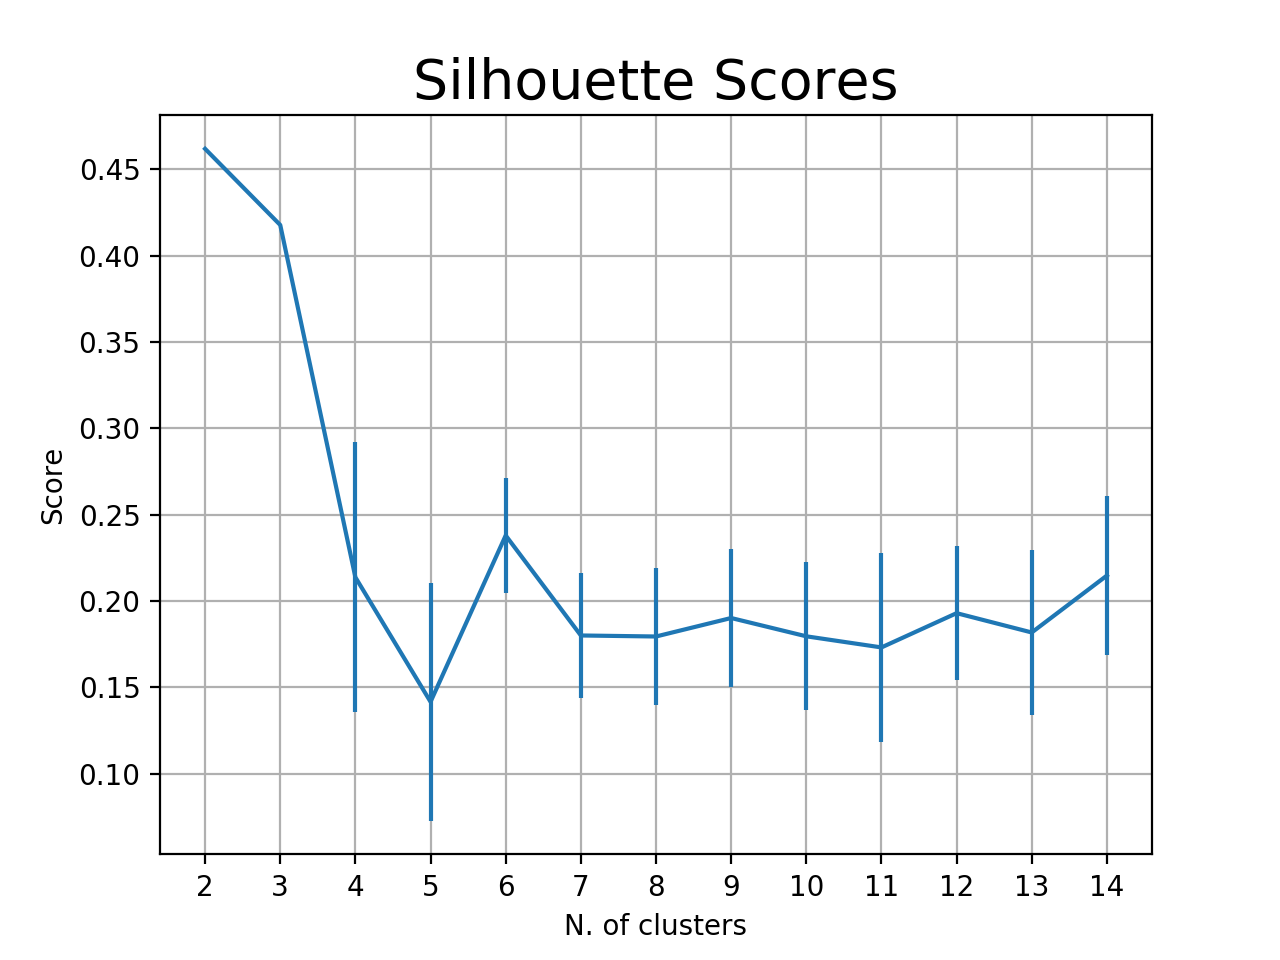
\includegraphics[width=.95\linewidth]{em_ica_dataset1_sil}
   \end{minipage}\hfill
 \caption { Simulated Annealing Tuning}
\end{figure}
\textbf{K means } 


\textbf{ Random Projection} Random projection is another dimensionality reduction method used to project ’n’ total features into k-dimensional space where k is less than k. The main criteria used to select the k is the reconstruction error where the complexity is traded for accuracy of reconstruction. Main benefit of projecting the data this way is to lower dimensions and help save computation cost. Different random seeds were tried in the random projection and the reconstruction error is plotted for them . The plot is taken which has the lowest reconstruction error and for the dimensionality reduction the reconstruction error is put at 5 percent ( which is calculated by comparing with the maximum value and the value at which the components are selected). so the number of components taken are 24 for the first dataset. The random seed matter a lot in the random projection .
\textbf{Data set 1 visualisation} The dataset 1 visualisation is done for 2 components for the purpose of analyzing the data using the first two components from the random projection , as only 2 components are used the reconstruction error is very high and also we can see that there is not much to separate the data which all seems the same.

\begin{figure}[!htb]
   \begin{minipage}{0.33\textwidth}
     \centering
     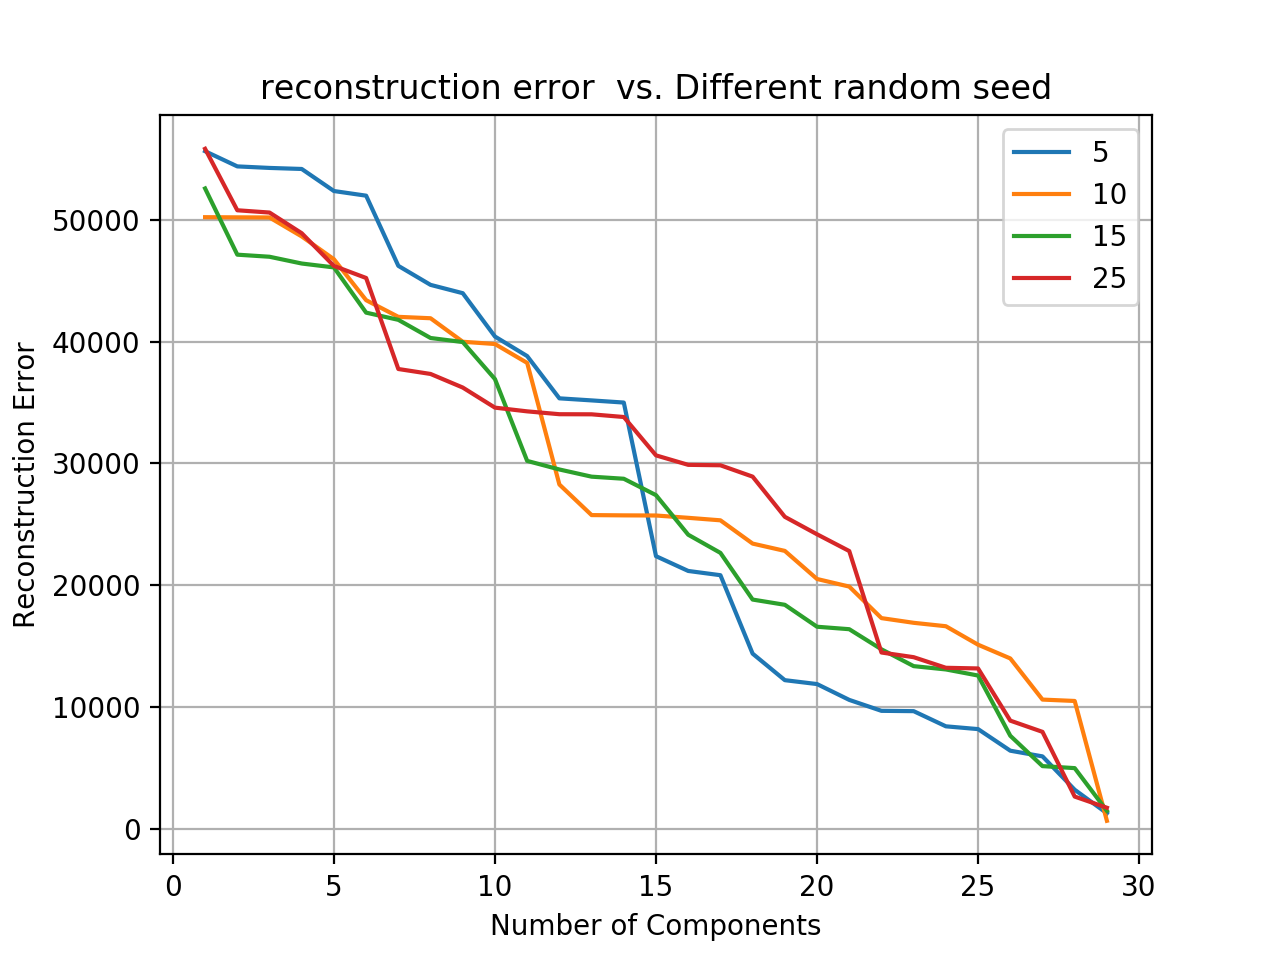
\includegraphics[width=.95\linewidth]{rp_dataset1}
   \end{minipage}\hfill
    \begin{minipage}{0.33\textwidth}
     \centering
     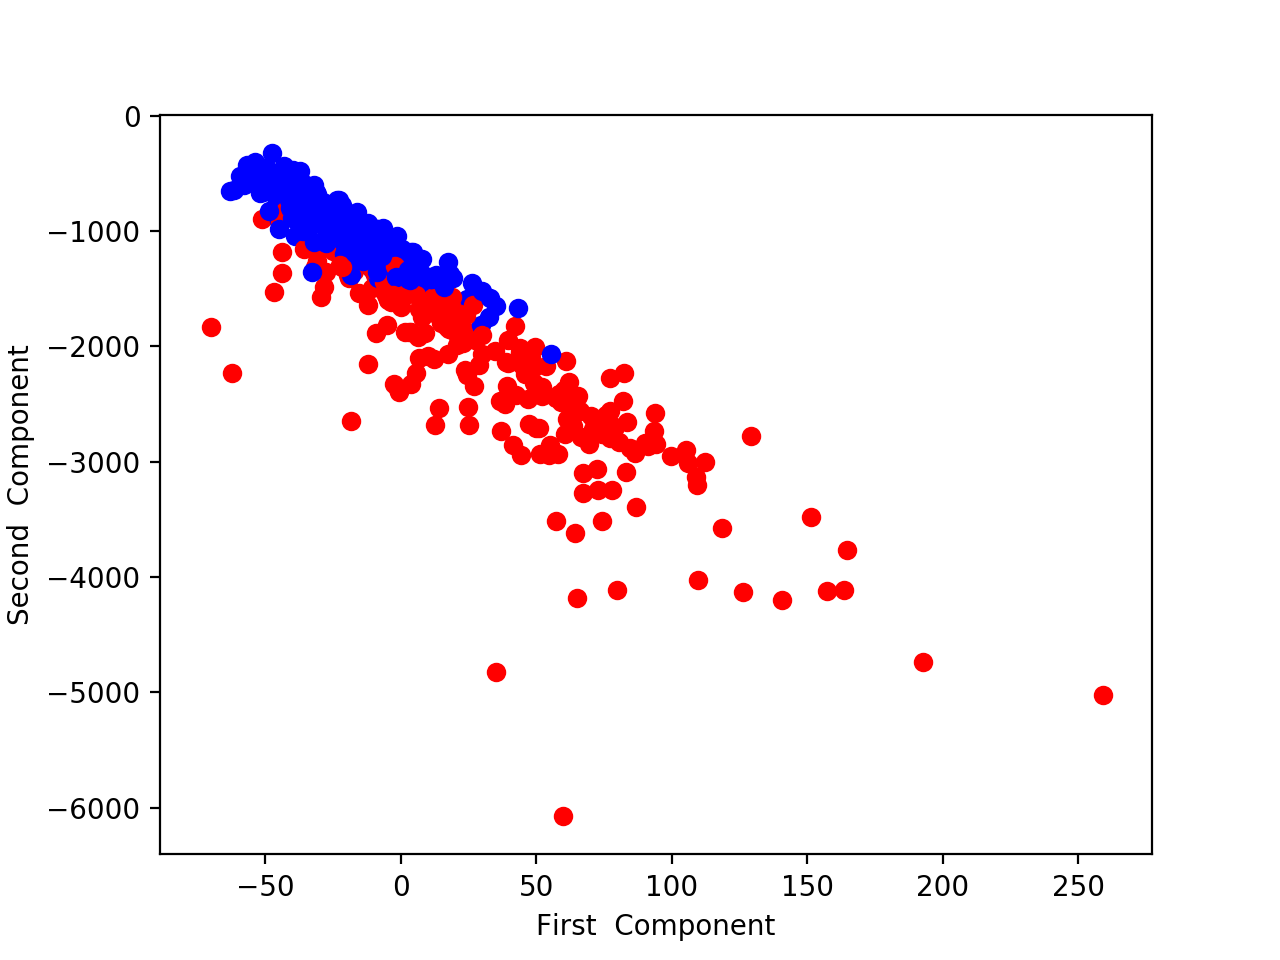
\includegraphics[width=.95\linewidth]{rp_dataset1_visual}
     \end{minipage}\hfill
     \begin{minipage}{0.33\textwidth}
     \centering
     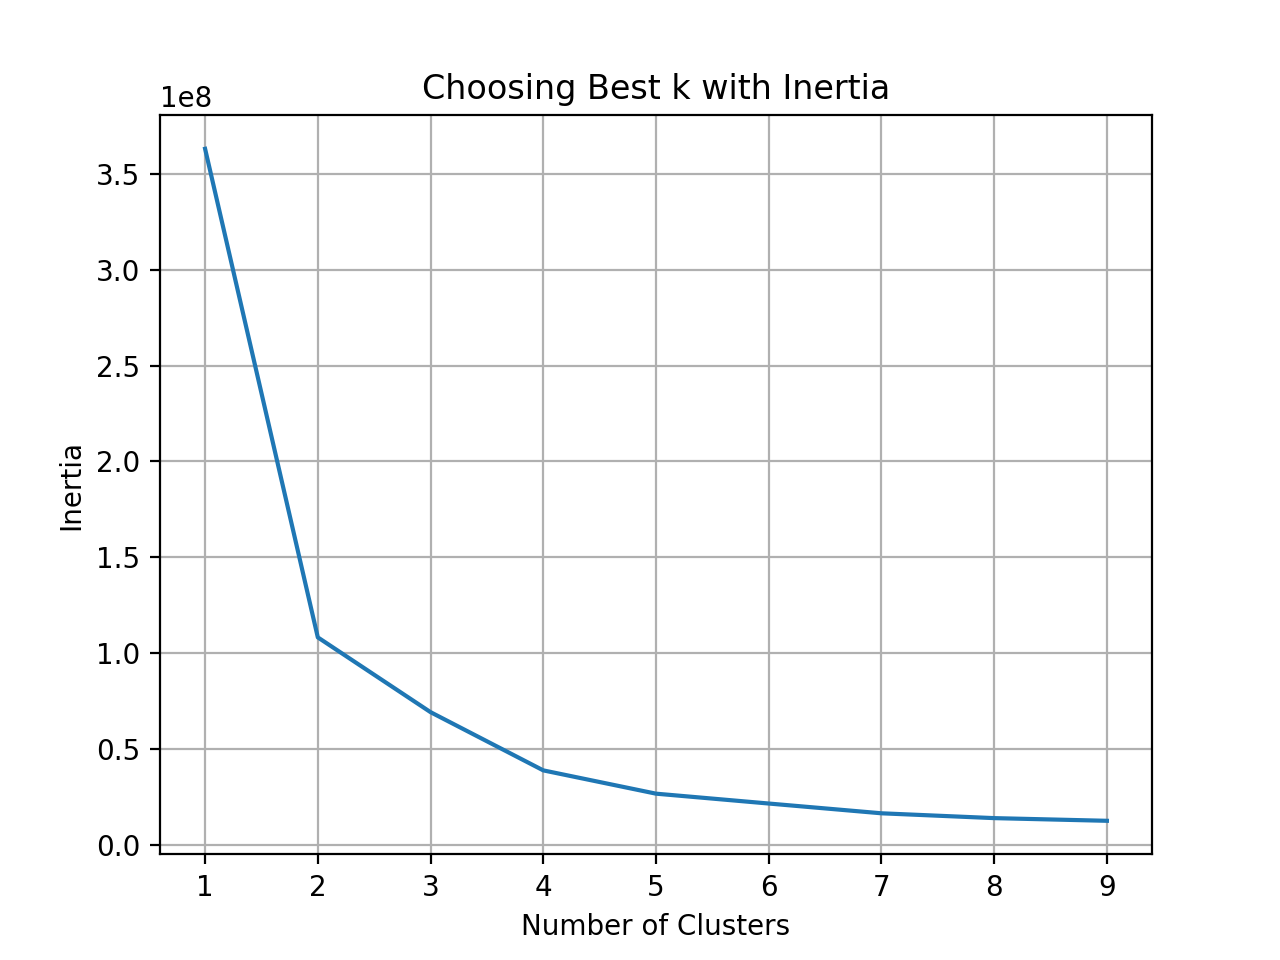
\includegraphics[width=.95\linewidth]{rp_clustering_dataset1_inertia}
   \end{minipage}\hfill
 \caption { Simulated Annealing Tuning}
\end{figure}

\begin{figure}[!htb]
   \begin{minipage}{0.33\textwidth}
     \centering
     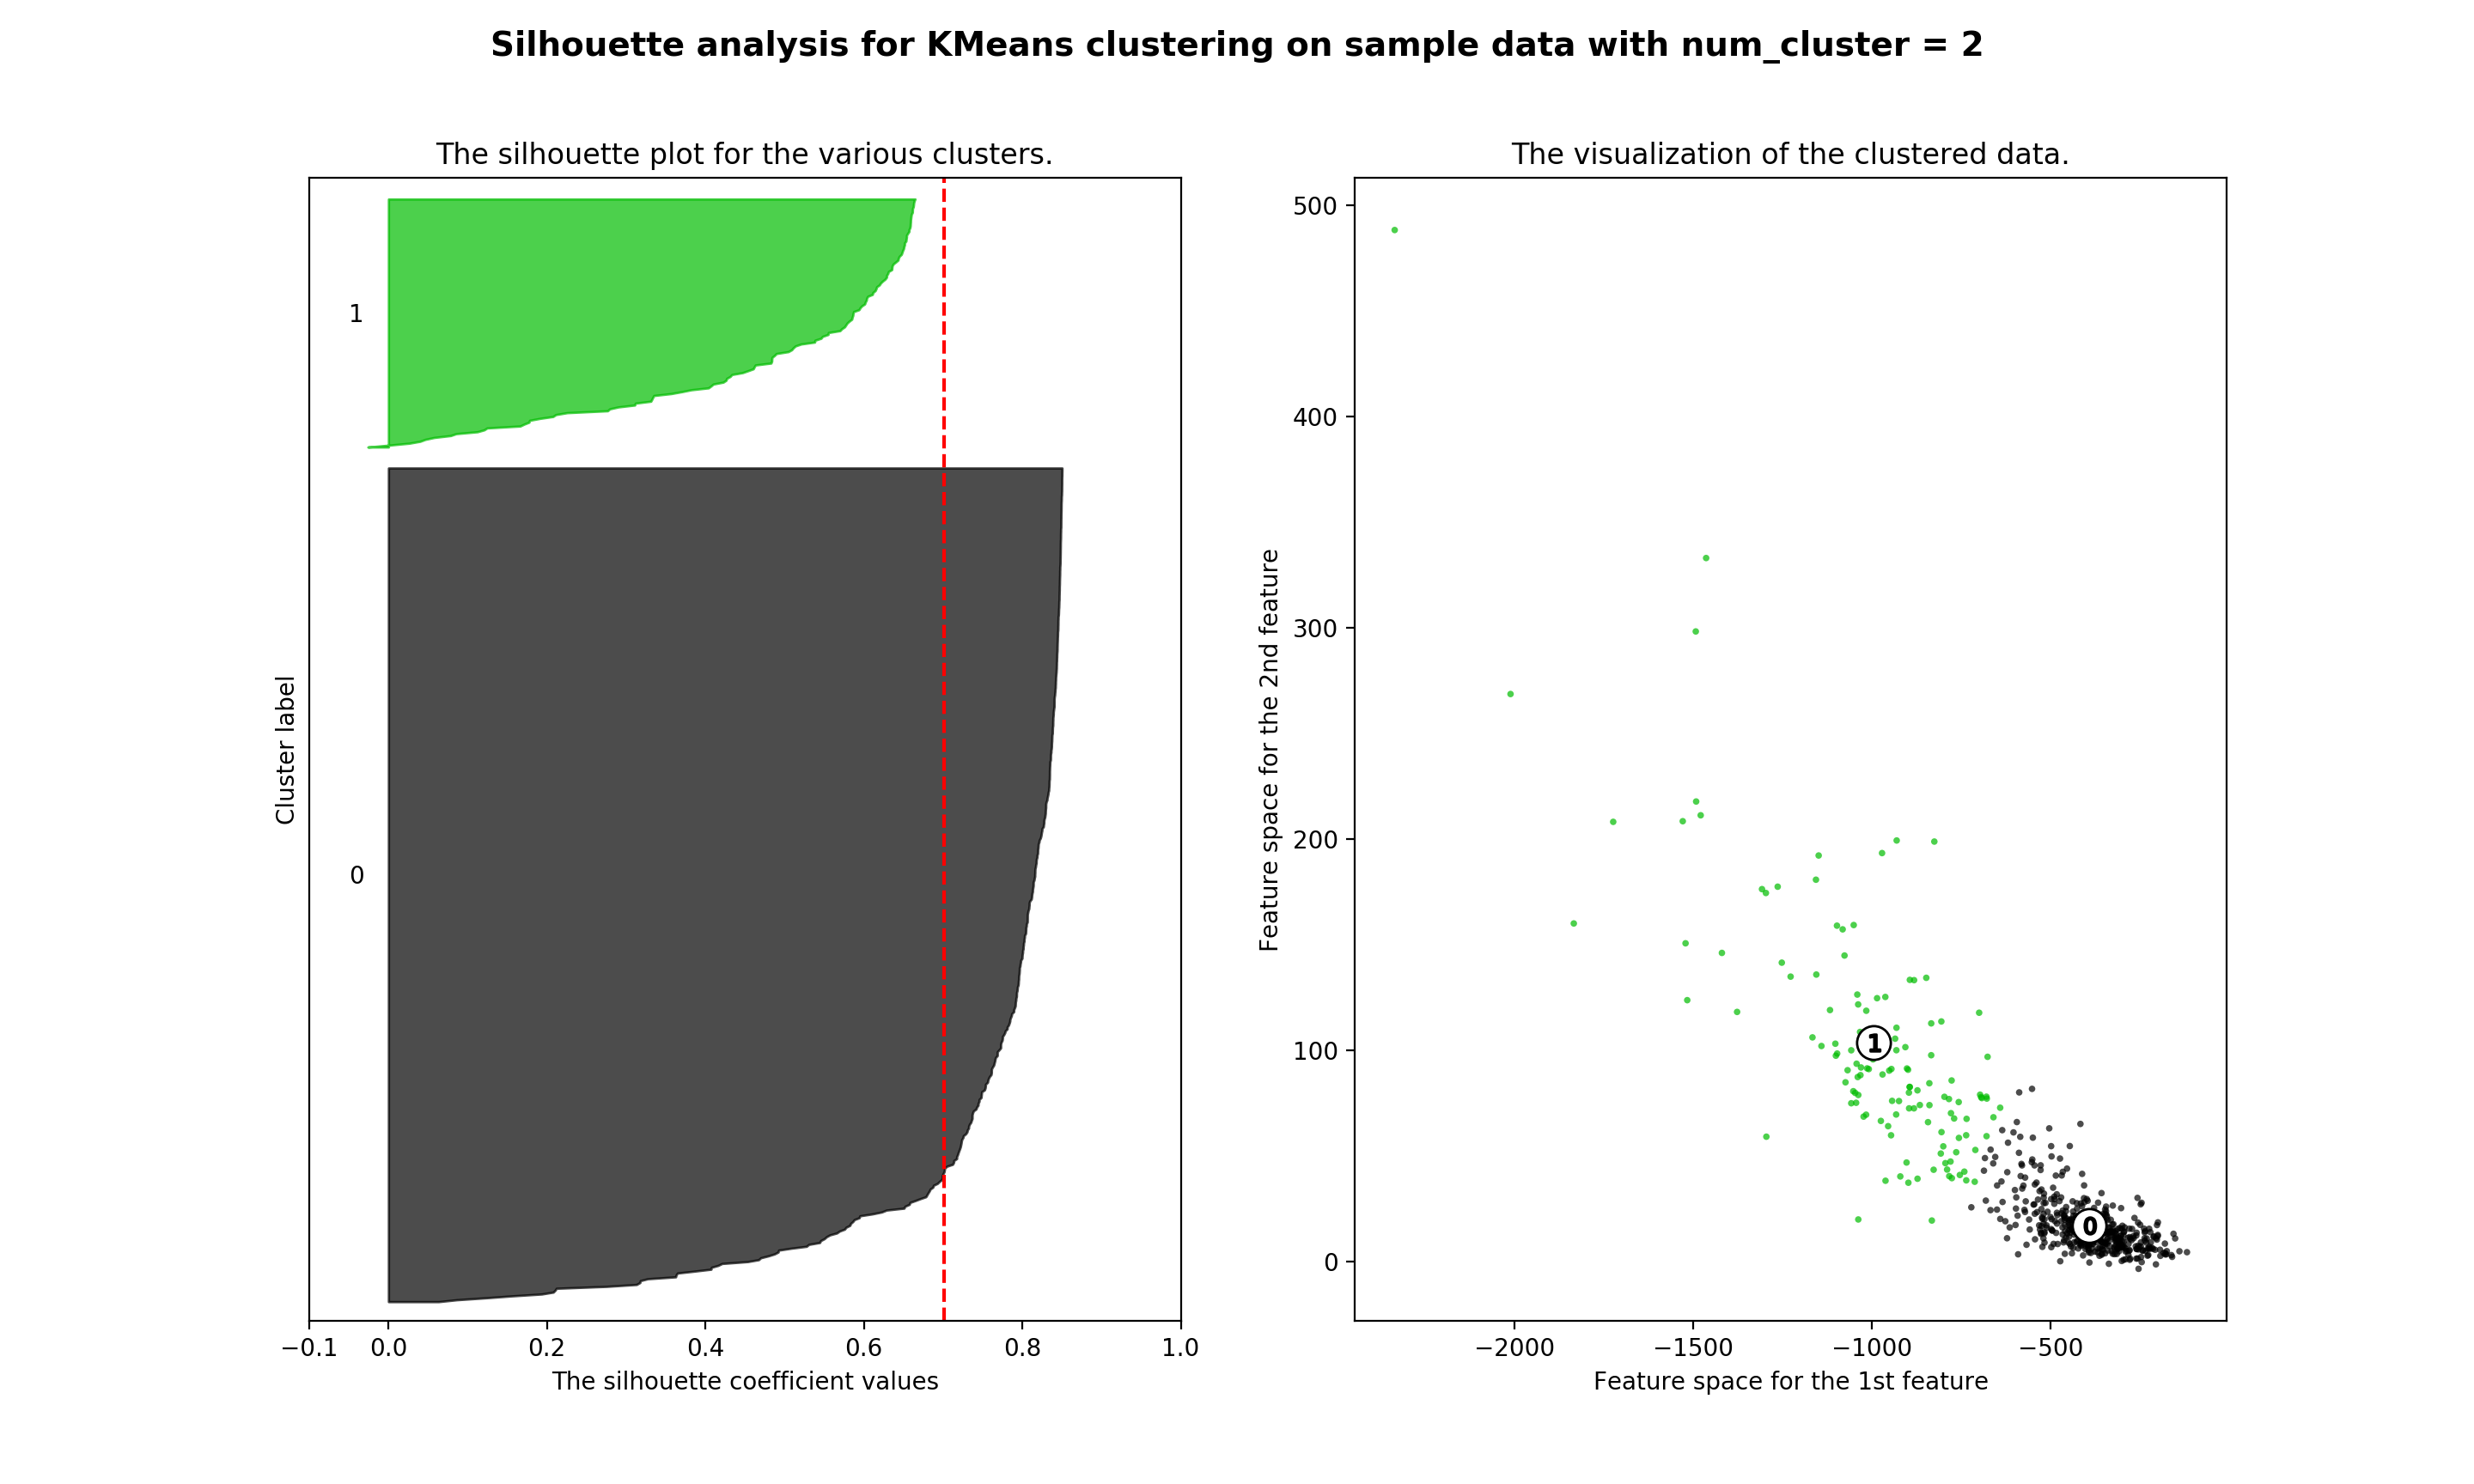
\includegraphics[width=.95\linewidth]{kmeans_rp_dataset_sil_vis}
   \end{minipage}\hfill
    \begin{minipage}{0.33\textwidth}
     \centering
     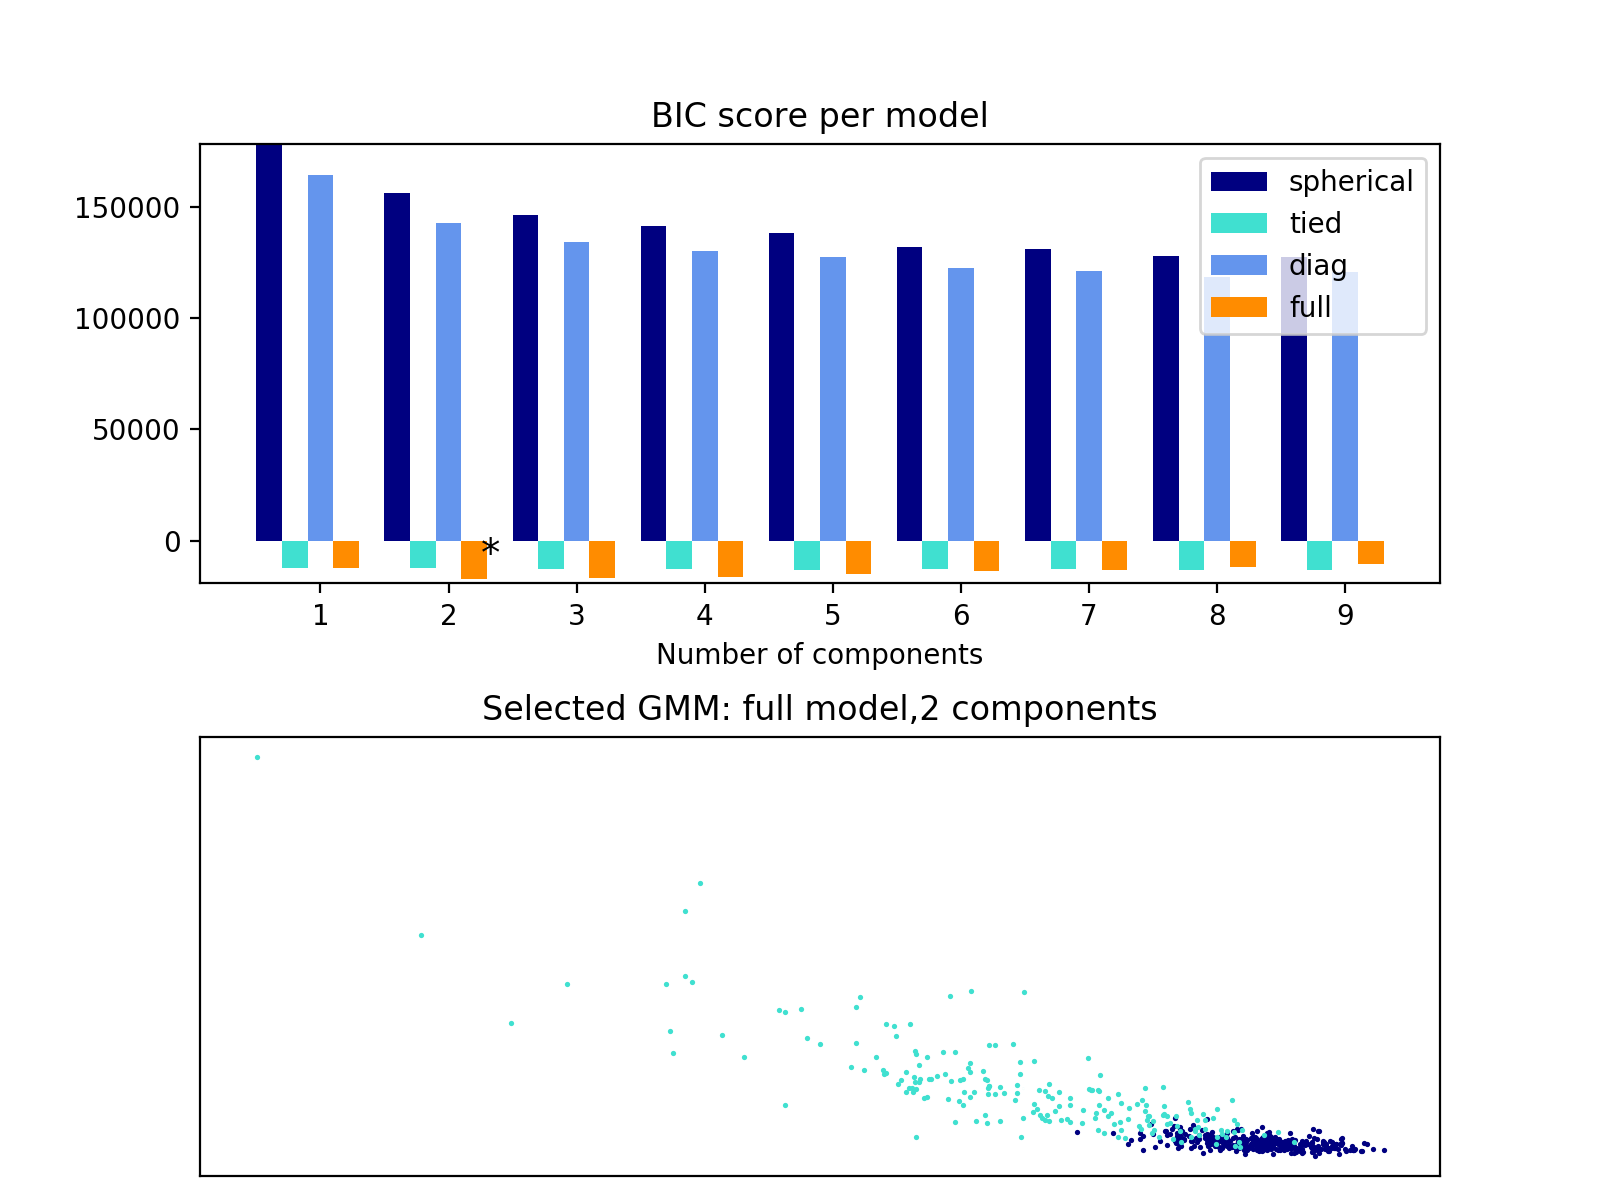
\includegraphics[width=.95\linewidth]{em_rp_dataset1_visual}
     \end{minipage}\hfill
     \begin{minipage}{0.33\textwidth}
     \centering
     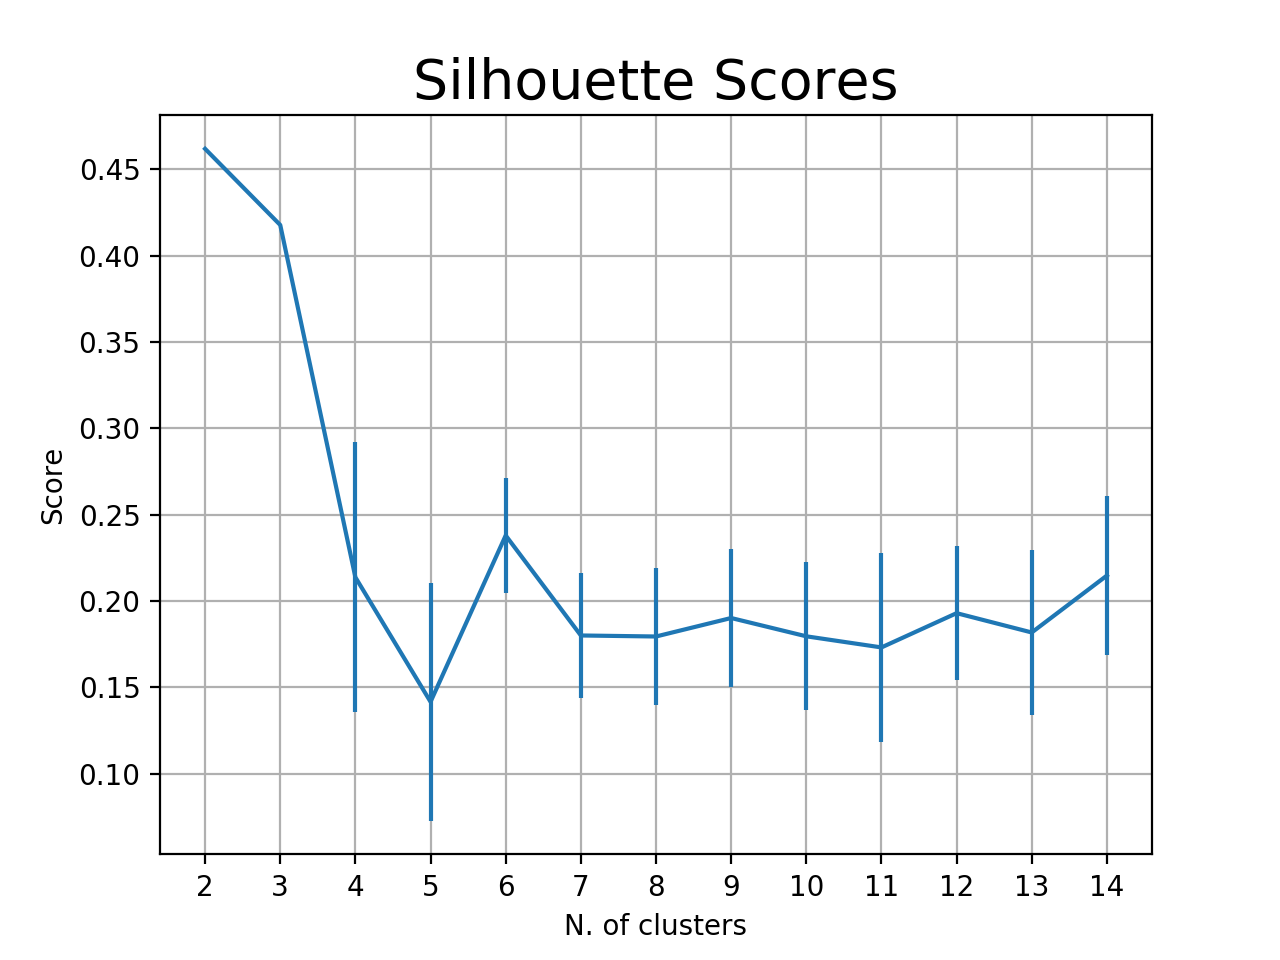
\includegraphics[width=.95\linewidth]{em_ica_dataset1_sil}
   \end{minipage}\hfill
 \caption { Simulated Annealing Tuning}
\end{figure}


\textbf{Kmeans Clustering} The kmeans clustering performed after the dimensionality reduction using the random projection shows great improvement in terms of the SA score and the accuracy criteria also. The value for the number of clusters is found to be 2 for the first dataset . The SA score came out to be 0.72 which is the highest in all the algorithms. the accuracy value for the kmeans clustering came out to be the largest at 85.6 percent. \newline 
\textbf{EM analysis} The expectation maximisation analysis done after  the random projection shows the same value as that of the kmeans which is 2 for the number of components and covariance type as full which is good as the labels are also same. The accuracy for the clustering done via EM is also done which came out to be 89.4 percent higher than kmeans as expected as it has a higher degree of freedom in clusters.
\begin{figure}[!htb]
   \begin{minipage}{0.33\textwidth}
     \centering
     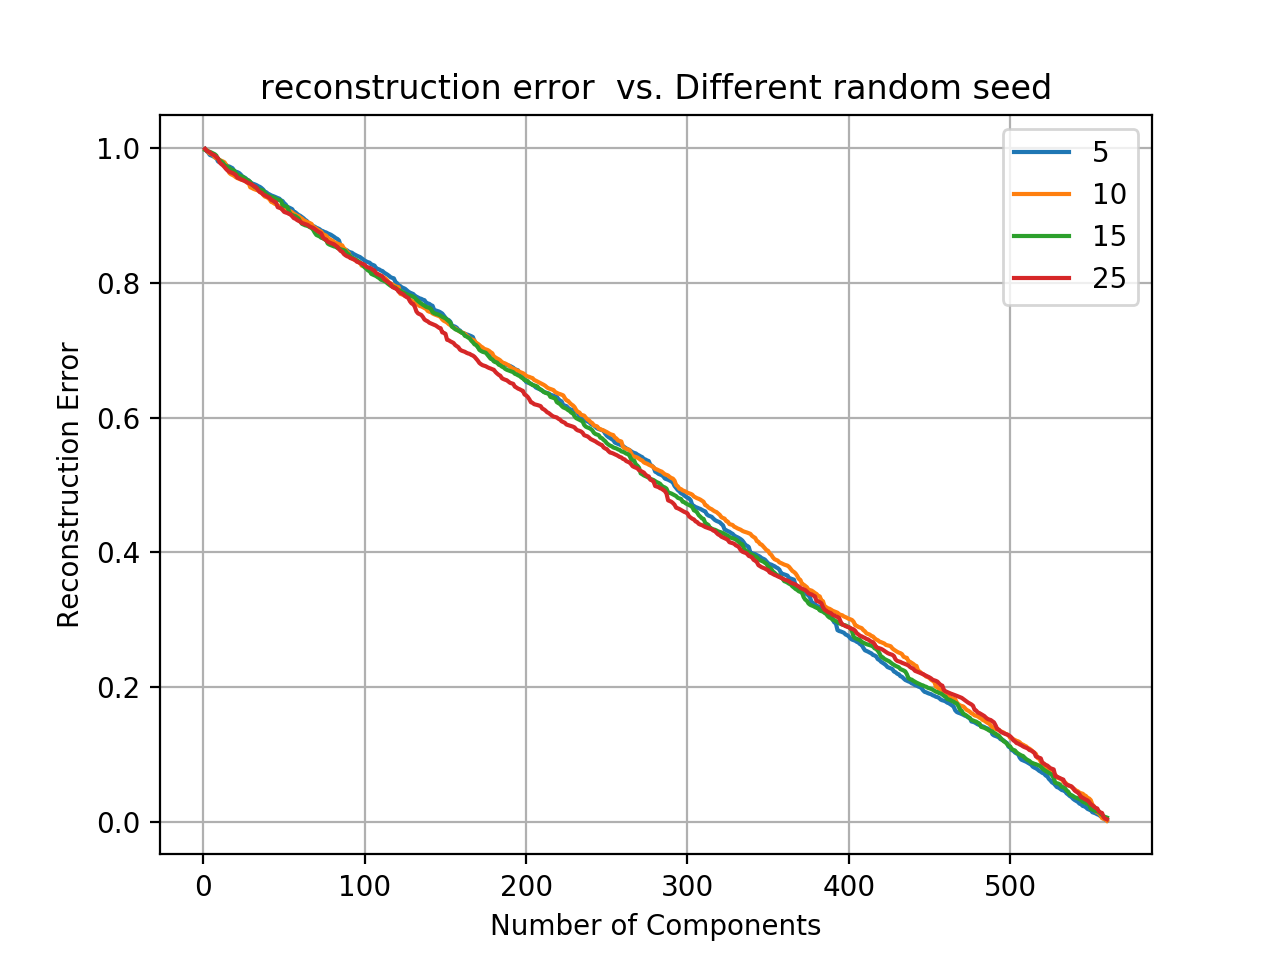
\includegraphics[width=.95\linewidth]{rp_dataset2}
   \end{minipage}\hfill
    \begin{minipage}{0.33\textwidth}
     \centering
     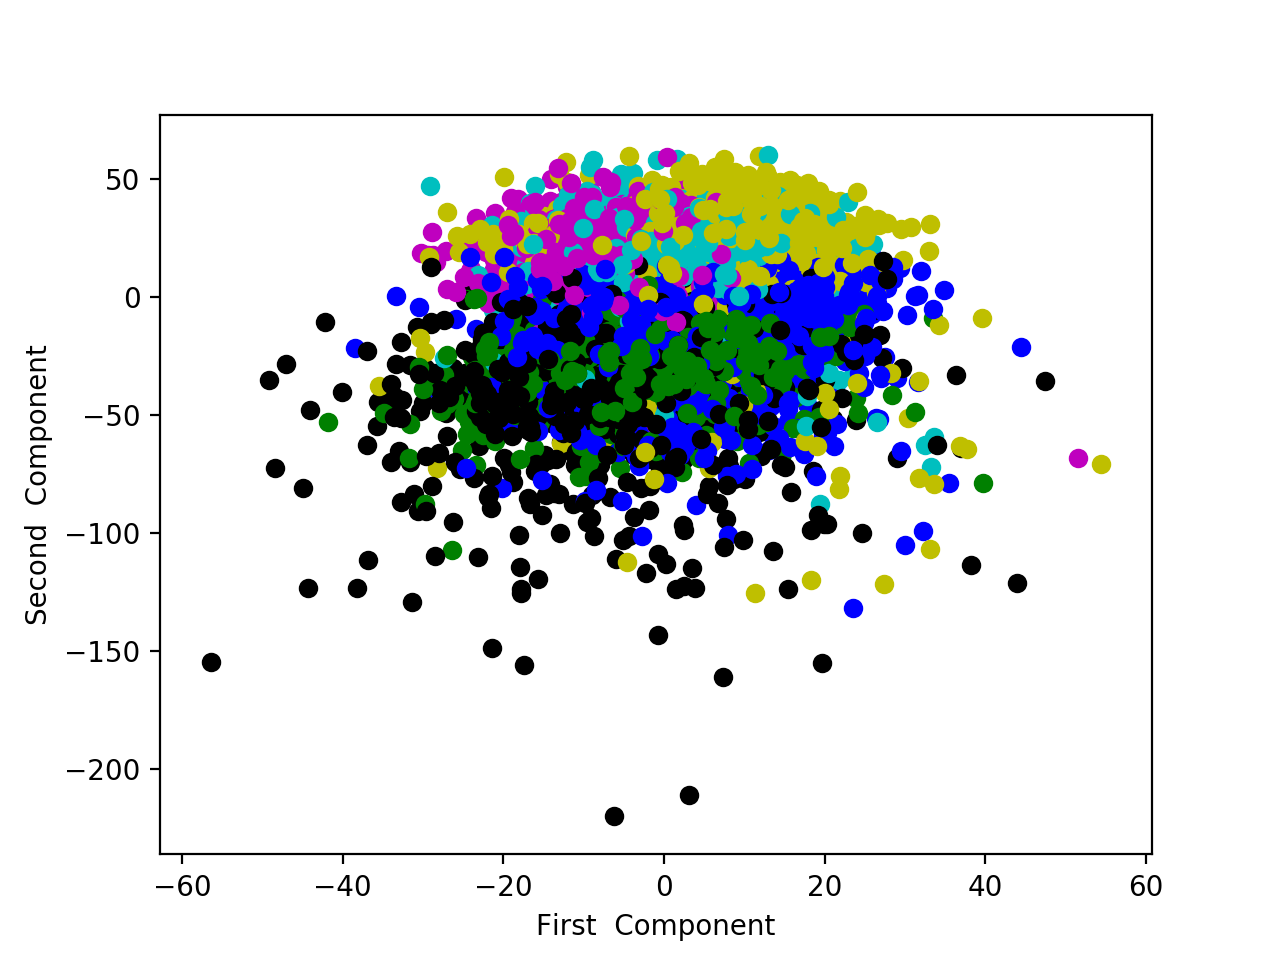
\includegraphics[width=.95\linewidth]{rp_dataset2_visual}
     \end{minipage}\hfill
     \begin{minipage}{0.33\textwidth}
     \centering
     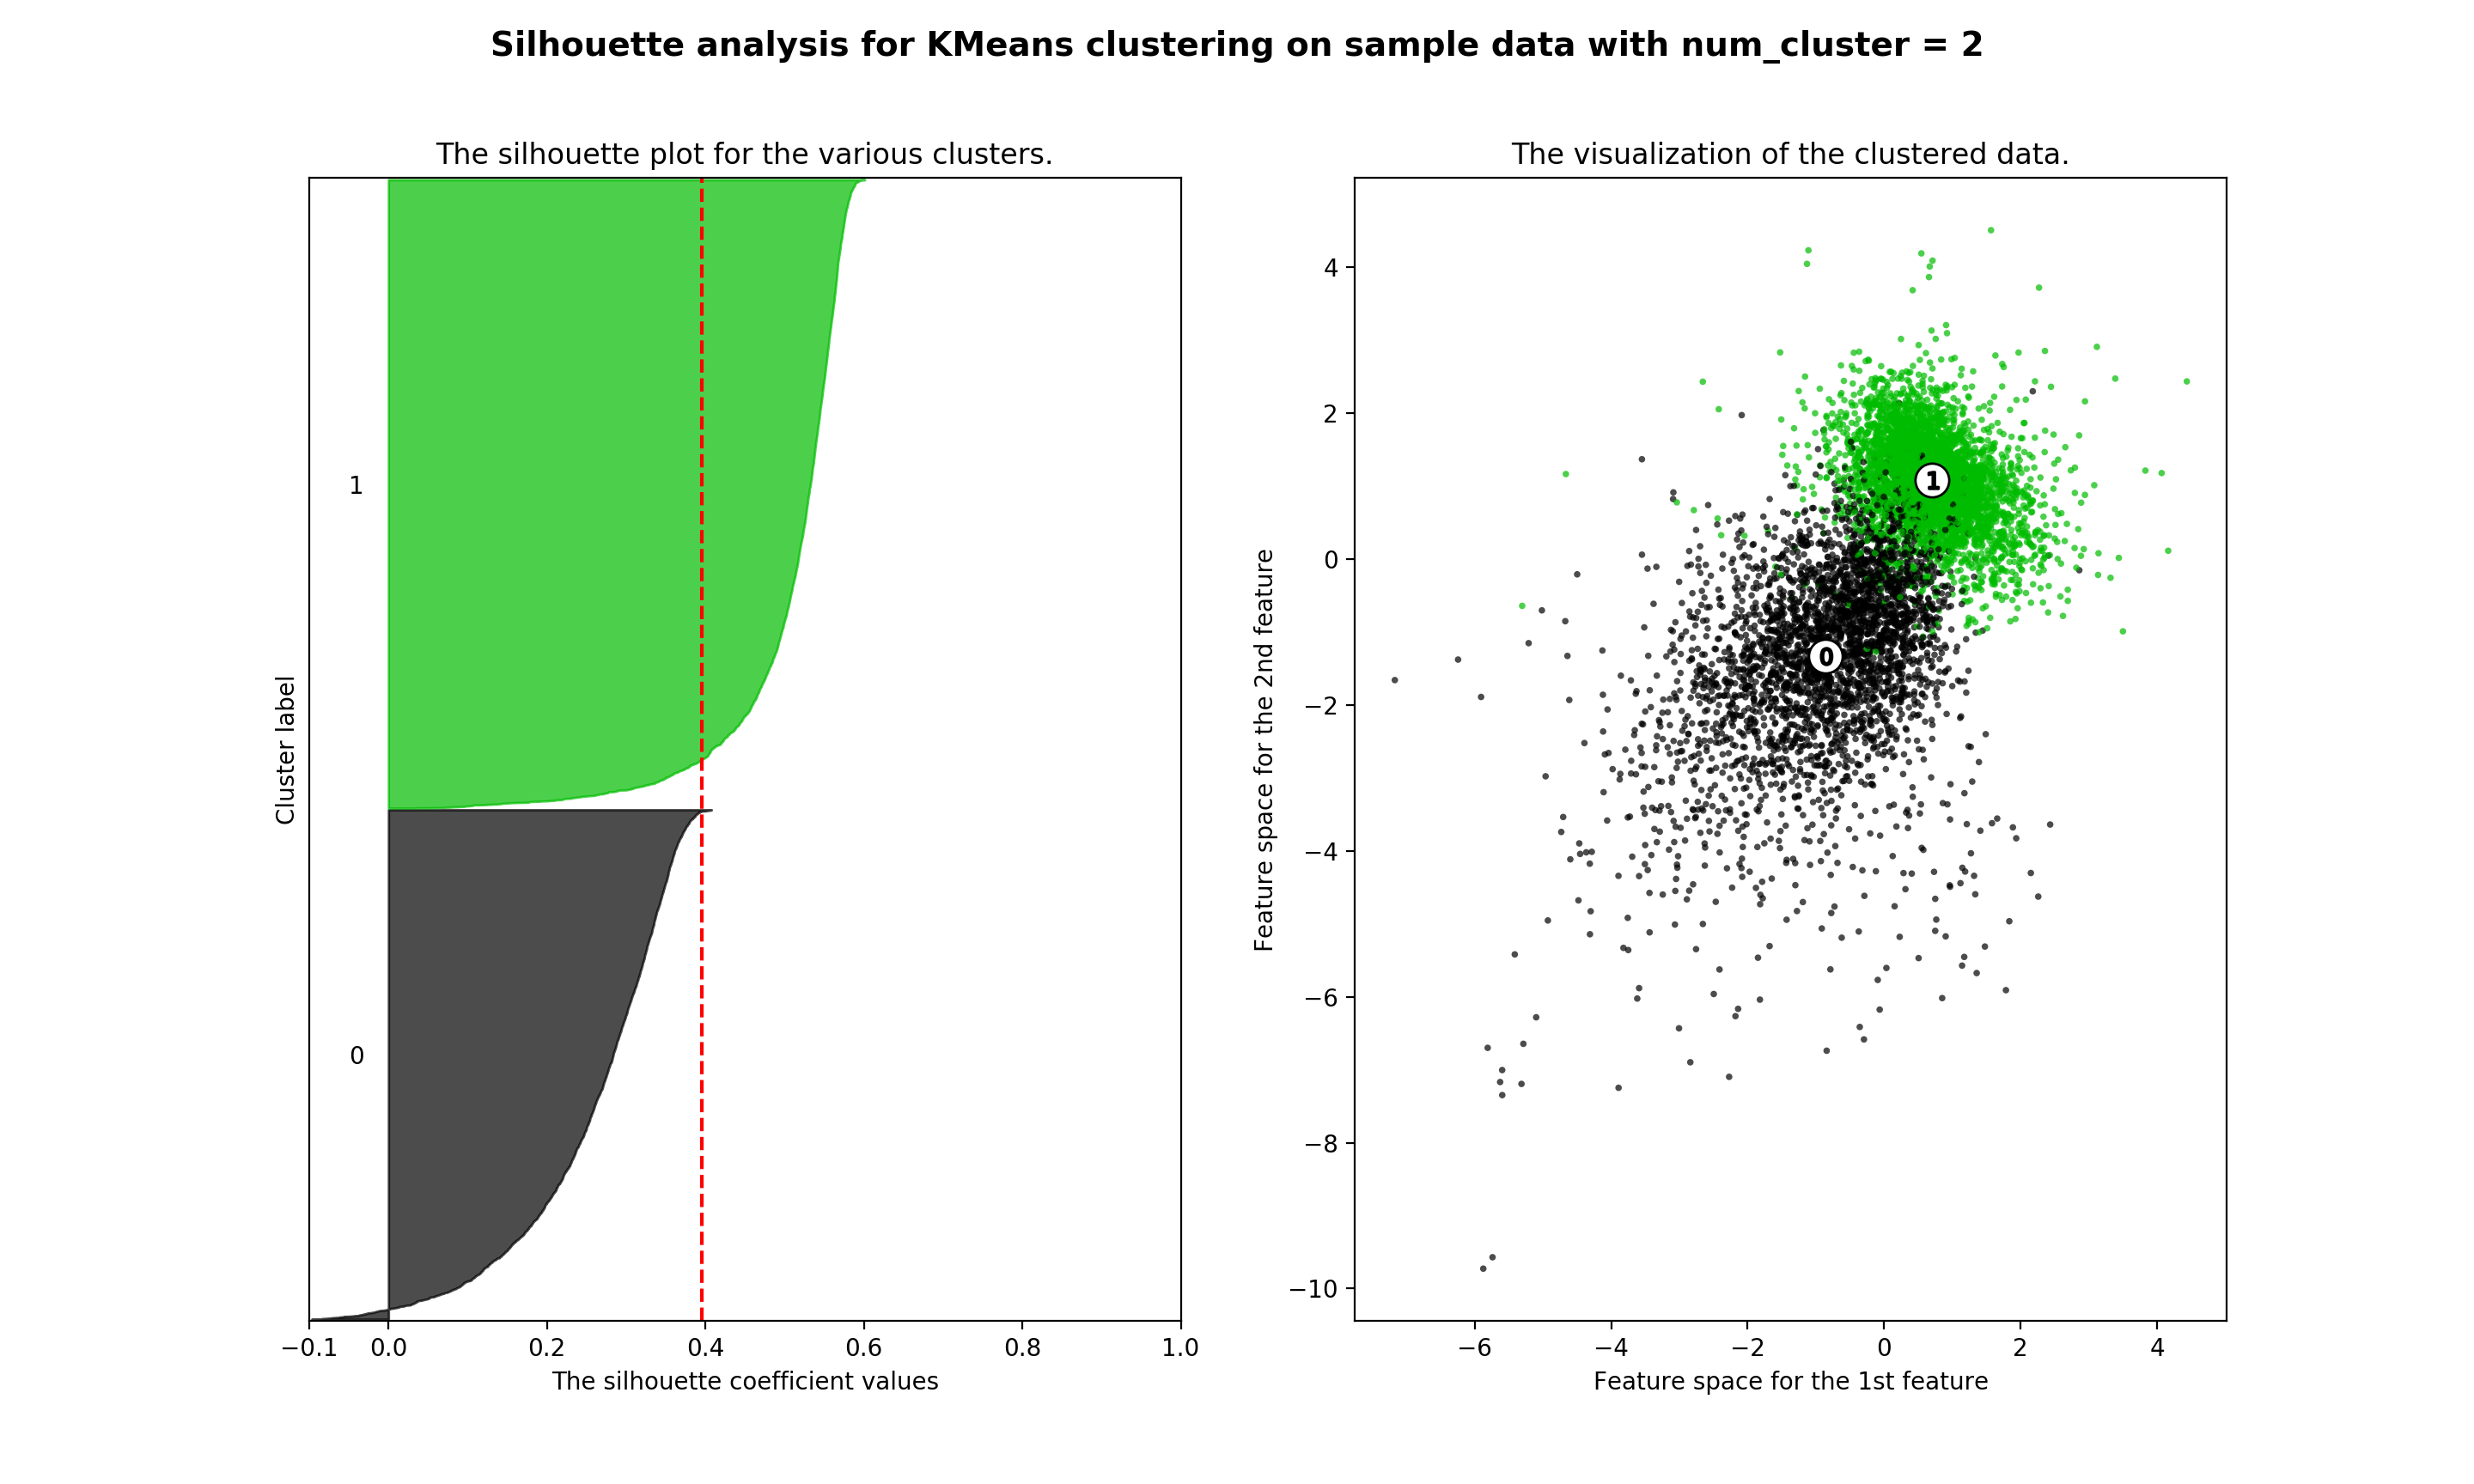
\includegraphics[width=.95\linewidth]{rp_dataset2_kmeans_visual_sil}
   \end{minipage}\hfill
 \caption { Simulated Annealing Tuning}
\end{figure}


\textbf{ Dataset 2} The random projection analysis done for the dataset 2 shows that the random seed has not much effect on the reconstruction error as all the curves have coincided this is due to the dataset having a large number of features where the random effect is nulled with the features. The reconstruction error is fixed at 10 percent and depending on that the number of components are selected which came out to be 475. One more value is also tested 500 which has a still lower error. The data set visualisation is shown for the dataset by taking only 2 components and it is not a mess because the number of label's is 6 means multi class and the we are using only 2 components which is not good. 
\textbf{Kmeans}. The clustering done after random projections the number of clusters comes out to be 2 via SA analysis as for k=2 has the highest score of 0.396 while for  k=6 the score comes out to be 0.11 much less . why the number of cluster is coming out to be 2 is because of the data set as the activities or labels can be divided into sedentary and motion activities and the unsupervised algo's are able to pick them but are not able to distinguish further or go deeper. The increase in the number of components did not had an effect on the number of clusters. The accuracy came out to be much lower around 25 percent because the labels were reduced from 6 to 2 so accuracy didn't made sense in this case.

\begin{figure}[!htb]
   \begin{minipage}{0.33\textwidth}
     \centering
     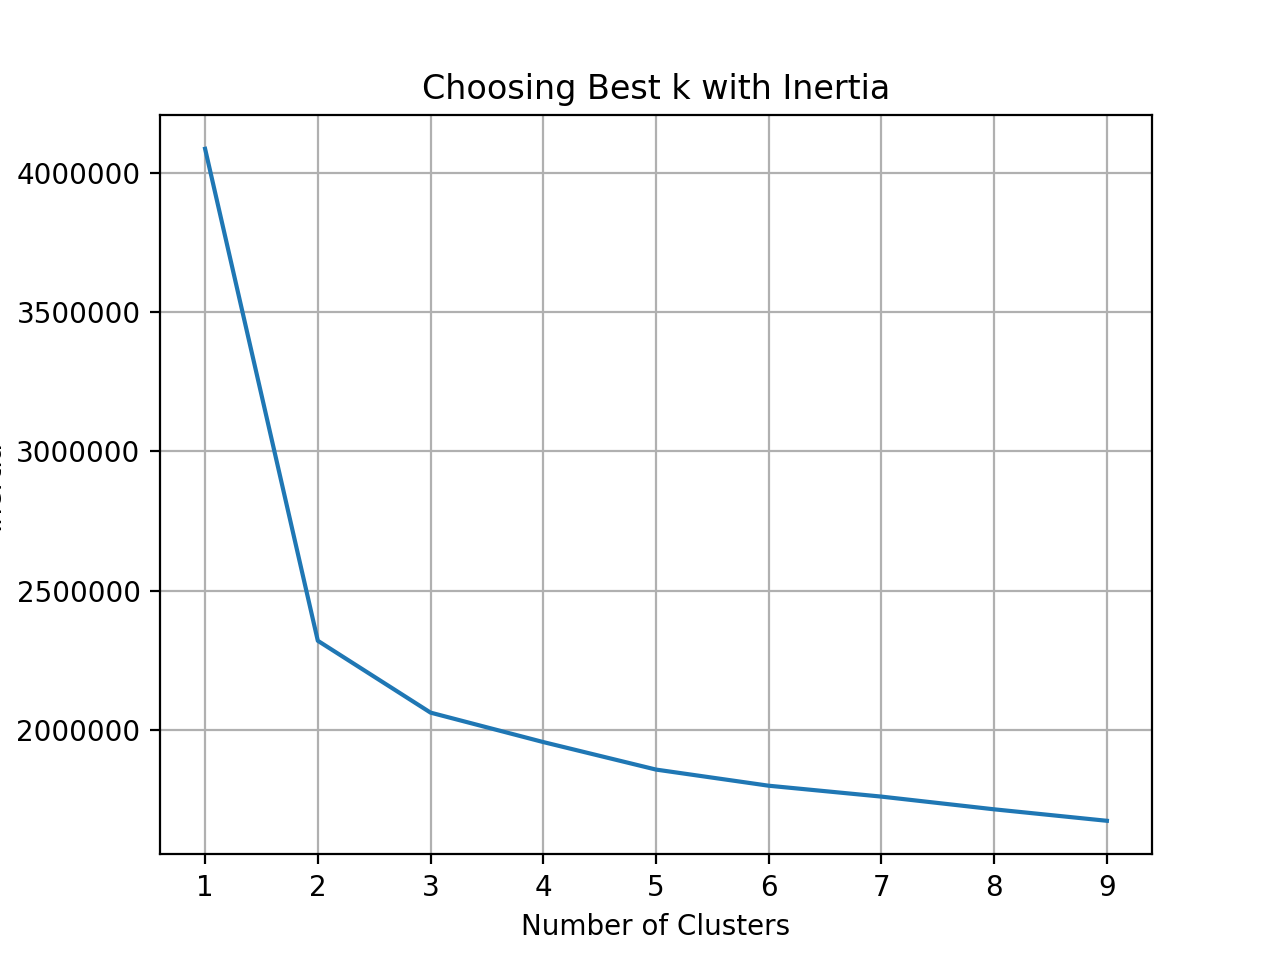
\includegraphics[width=.95\linewidth]{kmeans_rp_dataset2_inertia}
   \end{minipage}\hfill
    \begin{minipage}{0.33\textwidth}
     \centering
     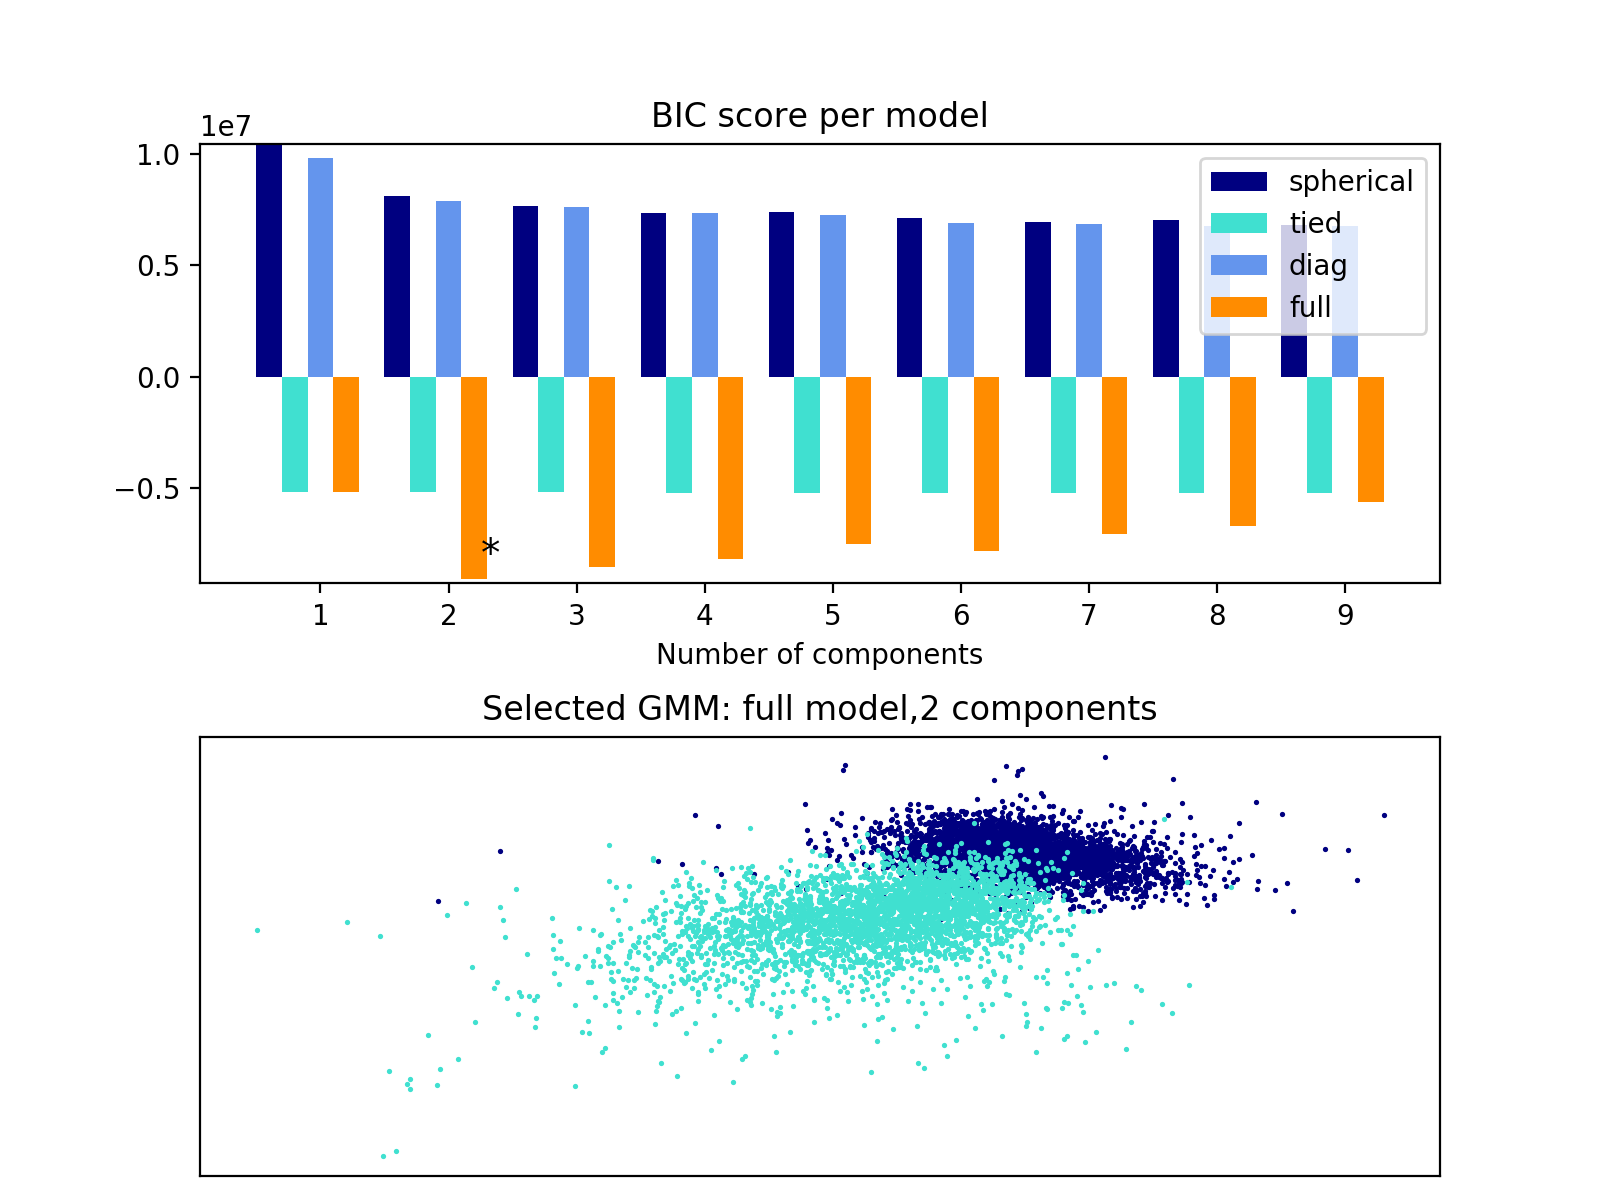
\includegraphics[width=.95\linewidth]{rp_dataset2_em}
     \end{minipage}\hfill
     \begin{minipage}{0.33\textwidth}
     \centering
     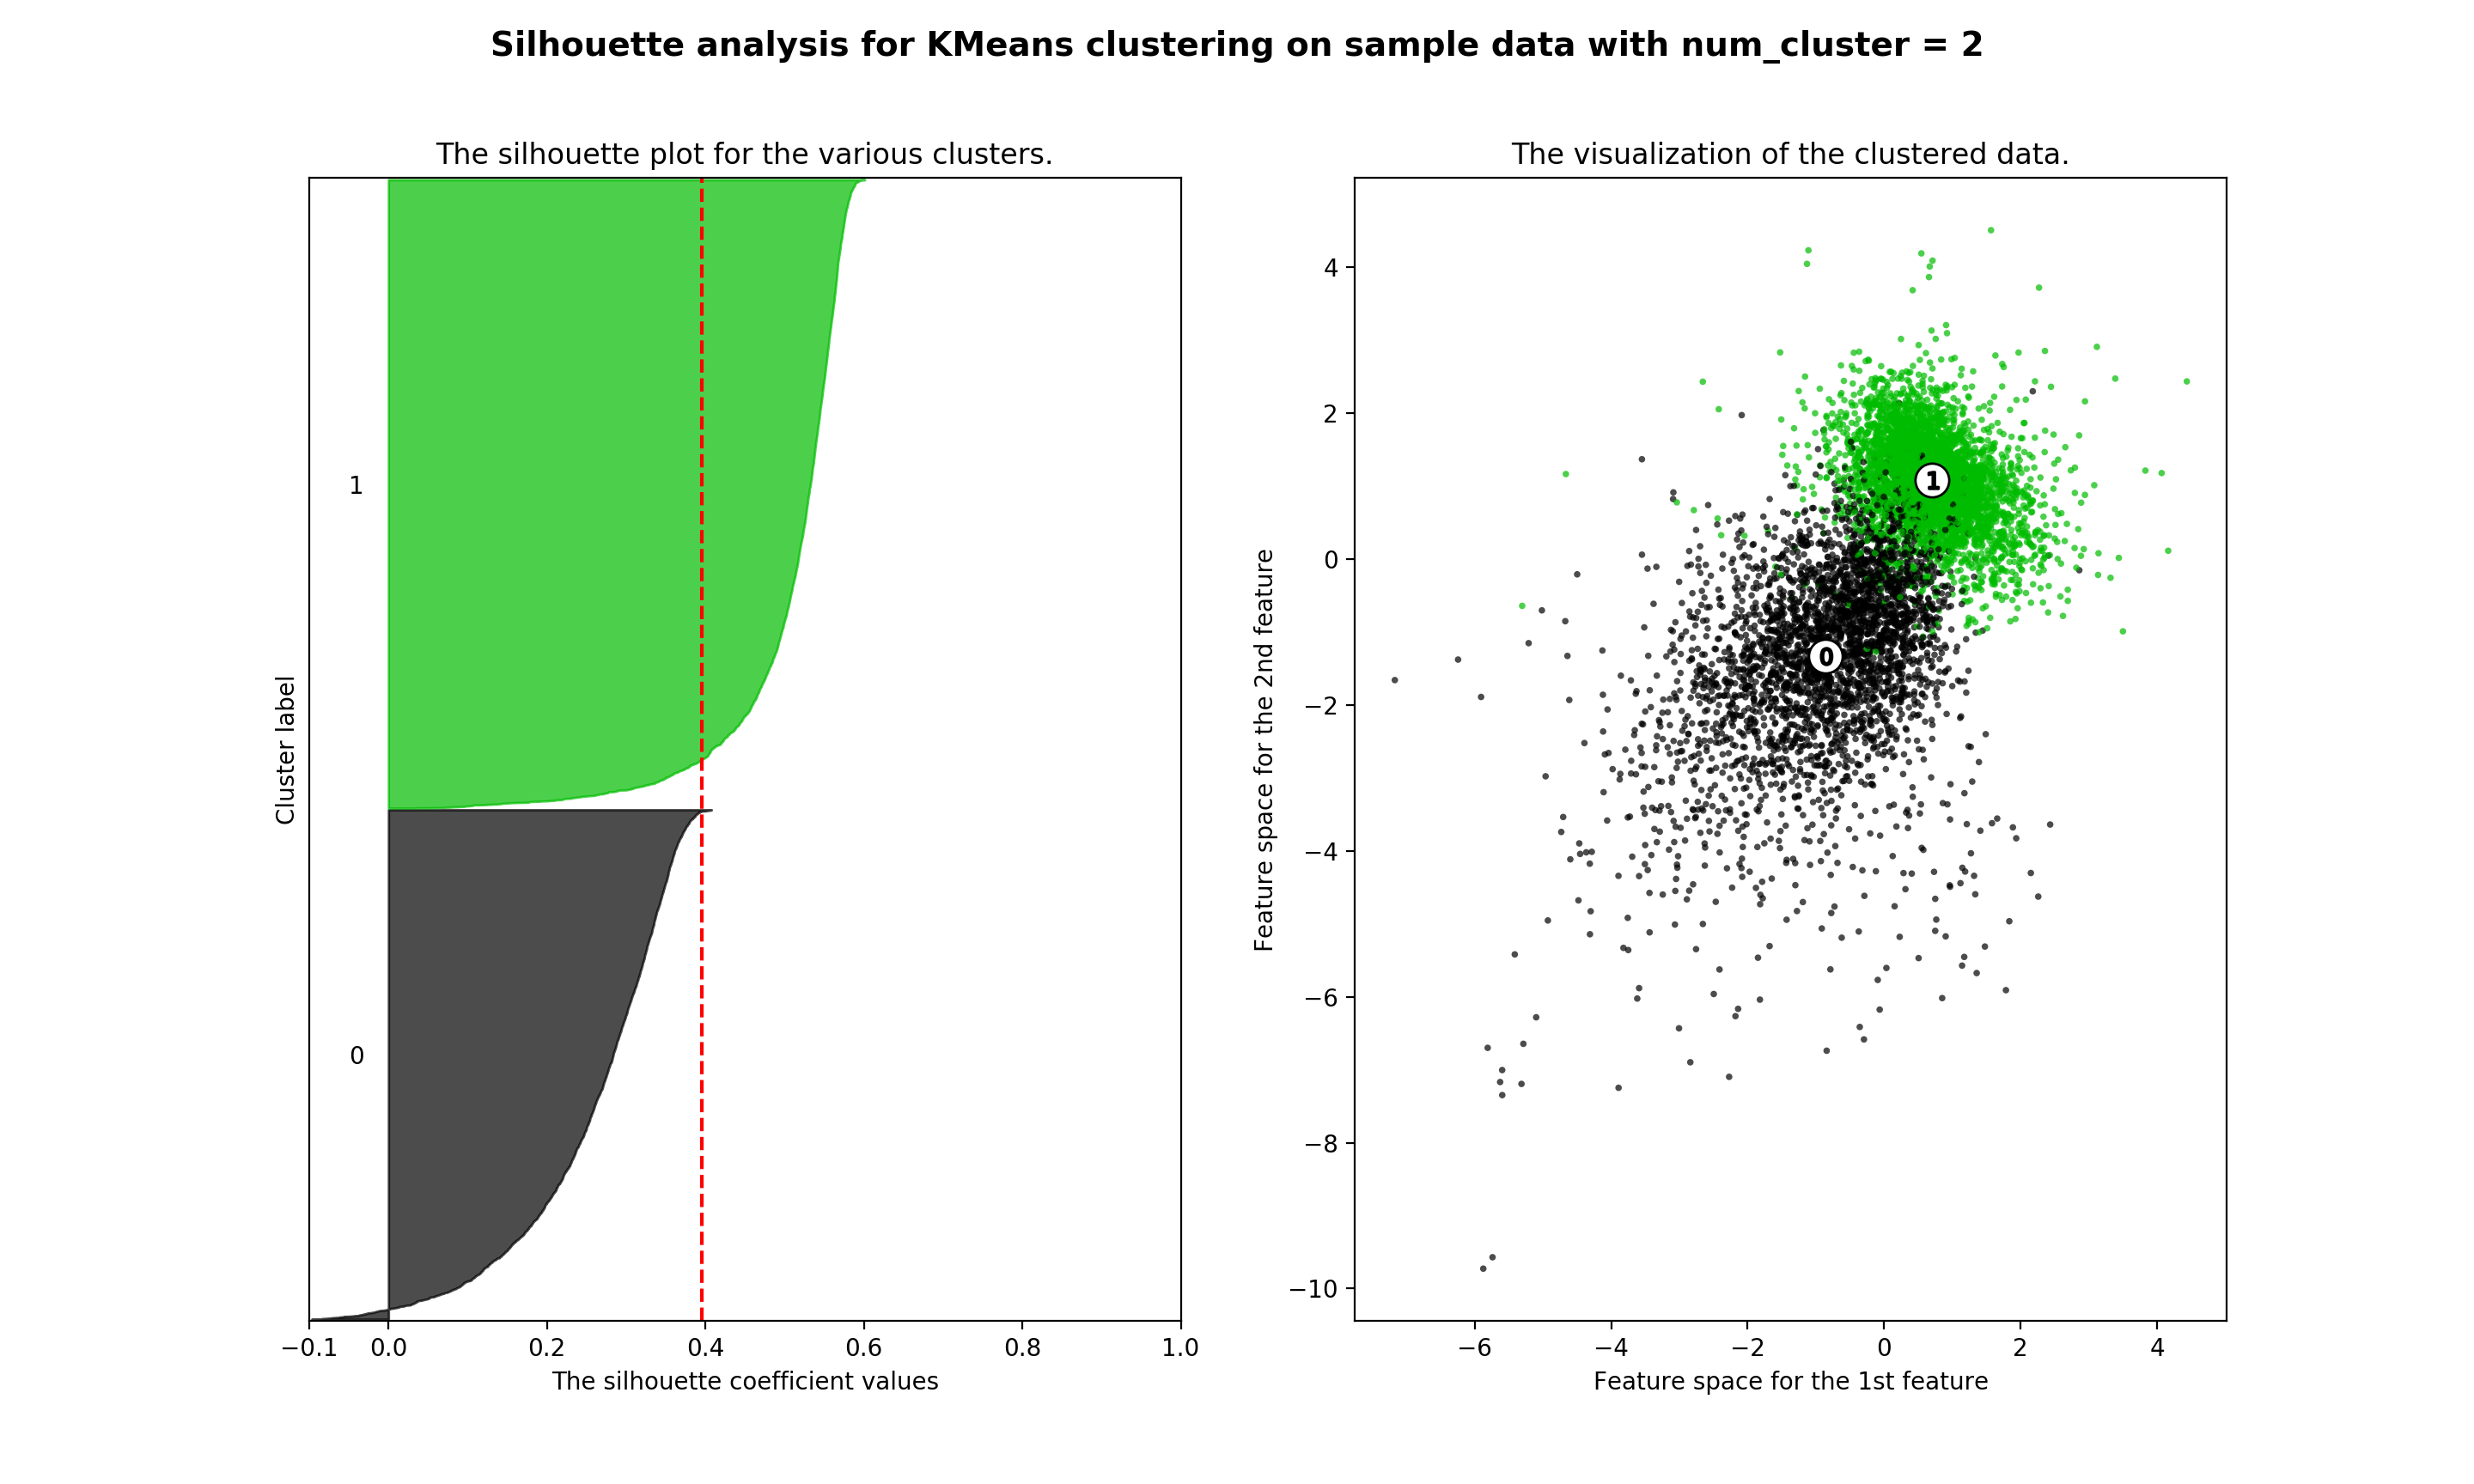
\includegraphics[width=.95\linewidth]{rp_dataset2_kmeans_visual_sil}
   \end{minipage}\hfill
 \caption { Simulated Annealing Tuning}
\end{figure}


\textbf{EM analysis}  The EM clustering also found the number of components to be 2 and covariance type as full it a 


\section { Neural network }
\subsection{ Dimensionality reduction and neural network }  For this analysis the breast cancer dataset is chosen and then the four algorithms are evaluated on the basis of accuracy , train time and testing time and the number of iterations . For the analysis forward search is done increasing the number of components one by one and then checking the mentioned parameters. For each algorithm the data is first transformed based on the number of components and then it is divided int training and testing set and then neural network learning is done on the resulting dataset. \newline 
\textbf{ Accuracy Analysis}The maximum accuracy achieved with the original dataset was 99.12 and the parameters of the neural network are not changed  for the dimensionality reduction algorithms, from the accuracy plot we can see that the PCA algorithm performs the best achieving the maximum accuracy within 4 algorithms and achieving it in least number of components and then the accuracy decreases with the increase in components for some time and this is due to addition of the unnecessary details and features  which makes the dataset more complicated and leads to overfitting due to which the accuracy decreases. \textbf{The random projection} shows the greatest variation going from 70 percent to 99 with the increase in the number of components which shows that the dimensionality reduction in the random projection will be less than other algorithms if we want the same accuracy. The Kbest has comparable accuracy and eventually achieves the maximum but it required a larger number of components than PCA and RP.  The ICA performed the worst of all the four algorithms and not achieving the maximum accuracy because it is not a blind source problem and the underlying features  were not independent and this was verified by plotting the correlation between the different features of the dataset and this is the reason ICA did not performed well. \newline
\textbf{ testing time} We have taken the optimum number of components for each algorithm for which they achieved the maximum accuracy and them compared the testing time at that value and it shows that randomized projection is the fastest of all followed by PCA and Kbest , the ICA has the maximum testing time also. 

\begin{figure}[!htb]
   \begin{minipage}{0.25\textwidth}
     \centering
     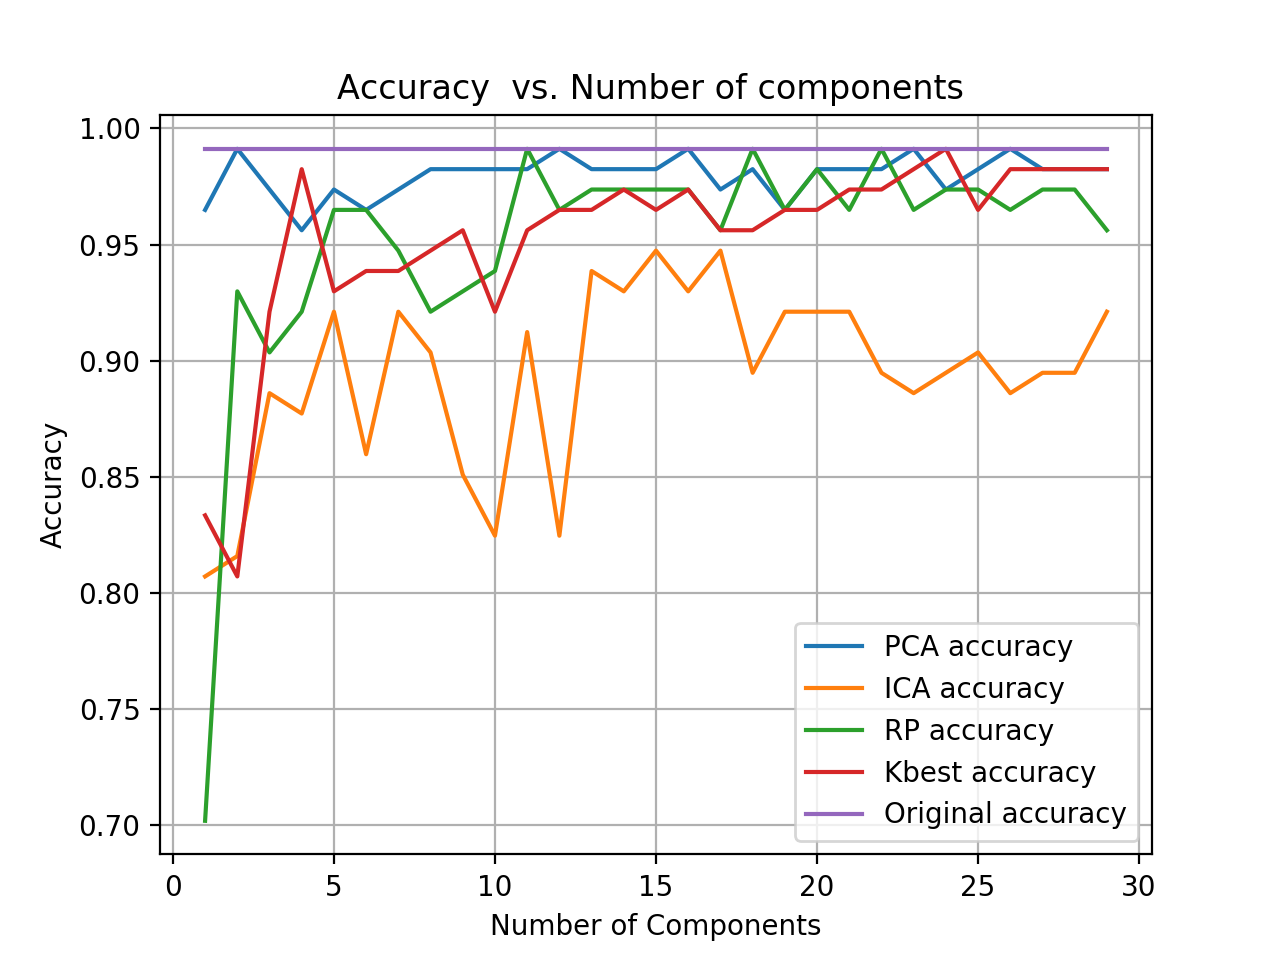
\includegraphics[width=.95\linewidth]{acc_neural_network_4}
   \end{minipage}\hfill
    \begin{minipage}{0.25\textwidth}
     \centering
     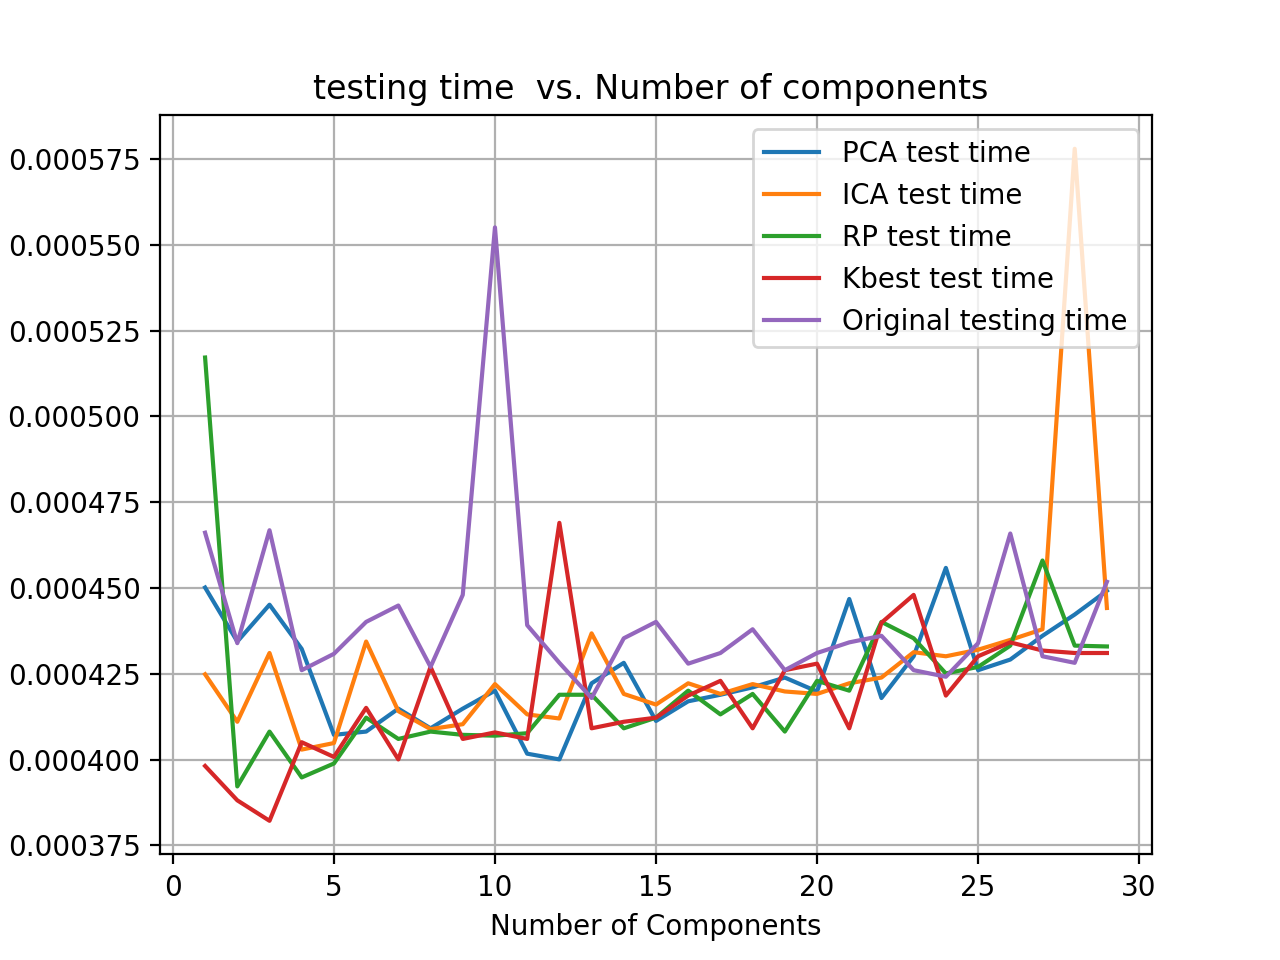
\includegraphics[width=.95\linewidth]{test_time_nn_4}
     \end{minipage}\hfill
     \begin{minipage}{0.25\textwidth}
     \centering
     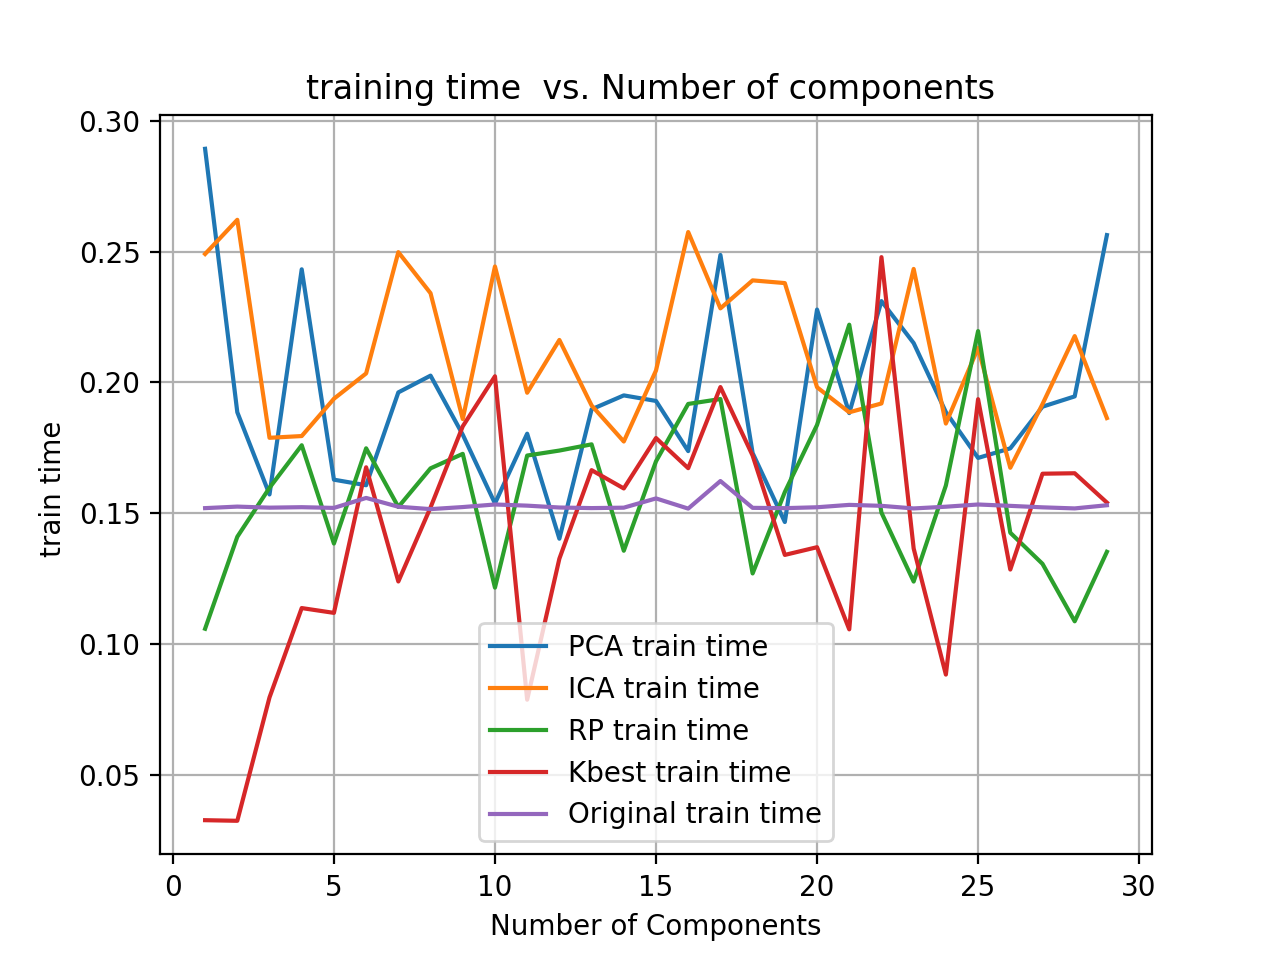
\includegraphics[width=.95\linewidth]{train_time_nn_4}
   \end{minipage}\hfill
    \begin{minipage}{0.25\textwidth}
     \centering
     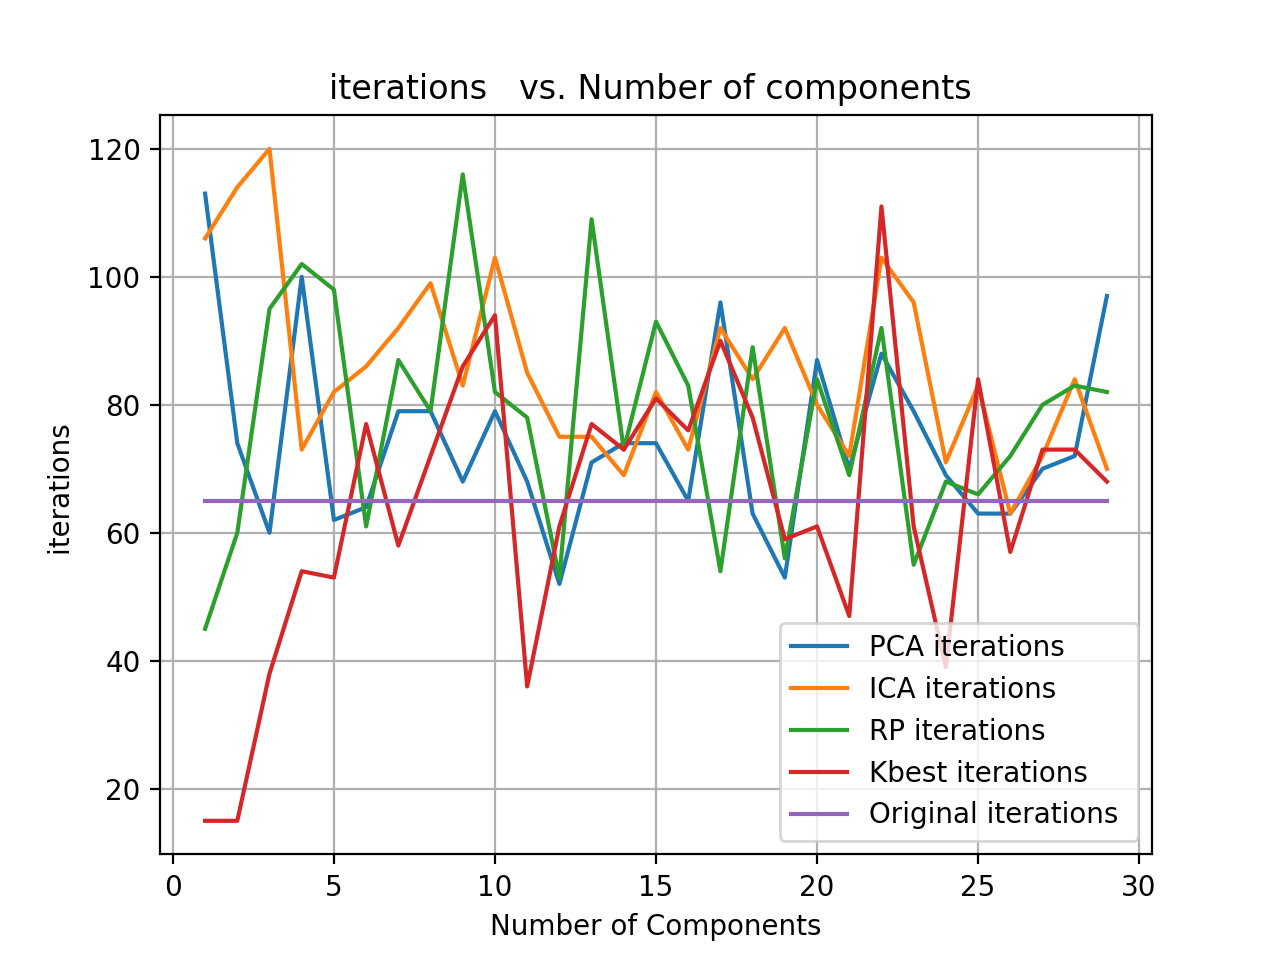
\includegraphics[width=.95\linewidth]{iter_nn_4}
   \end{minipage}\hfill
 \caption { Simulated Annealing Tuning}
\end{figure}

\subsection { Neural networks and clustering }  In this clustering is done first on the dataset and then the clustering labels were added as a feature to the dataset and then the neural network was run on the modified dataset. For the kmeans clustering the following parameters were plotted accuracy , train time , testing time and the number of iteration taken by the learner to converge so the highest accuracy achieved by the kmeans occurs at the cluster value of 2 and remain constant till 4 , the accuracy achieved is less than the accuracy achieved by the original data but the training time reduced from 0.15 sec in the original data to 0.12 and also the testing time is reduced half to 0.002 from 0.004 which means that the clustering can help up the supervised learning process and the reduction in accuracy is not that much which is reduced from 99 to 98.3.  The training time and the testing time increases with the increase in the number of clusters. The decrease in the accuracy can be attributed to the misclassification of some of the points by the clustering and the clustering labels becomes the dominant features in the modified training data which leads to decrease in the accuracy and decrease in training and testing time. The clustering can help to reduce the complexity of the model. \newline
\textbf{ EM Analysis } The expectation maximisation clustering algorithm was also run on the same dataset and evaluated on the same parameters , the accuracy was expected to increase using the em clustering but the maximum accuracy achieved using em also is same as that of kmeans because the data  is well separated and the shape of the data is not arbitrary due to which em and kmeans performs similarly on the accuracy. The training time and testing time is more for the em as compared with the kmeans because kmeans is easy and simpler compared to kmeans. The training time and testing time increased with the number of cluster and the accuracy decreased, this is due to the fact that increase in the number of clusters leads to the overfitting.
\begin{figure}[!htb]
   \begin{minipage}{0.25\textwidth}
     \centering
     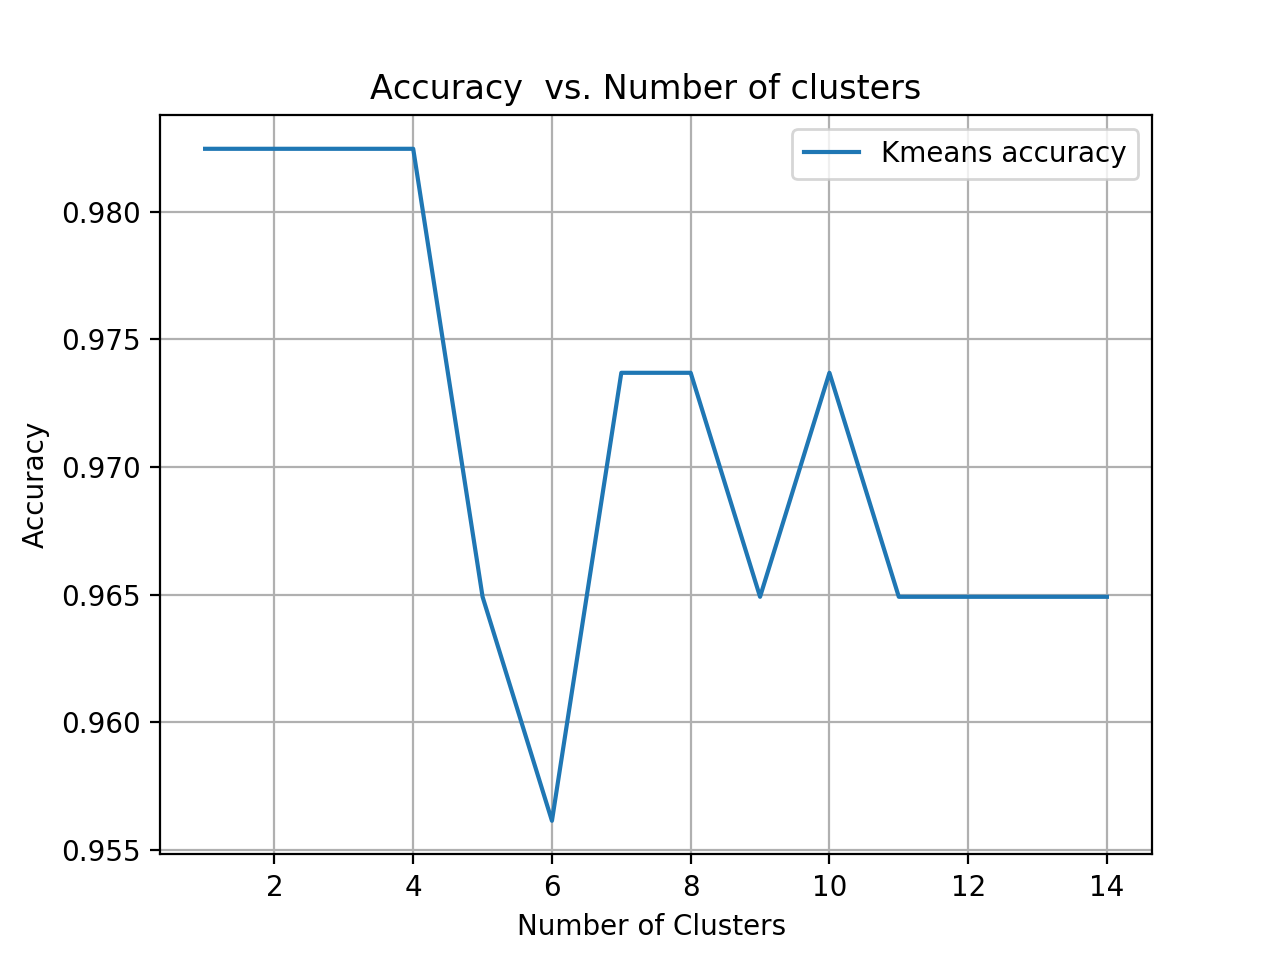
\includegraphics[width=.95\linewidth]{kmeans_nn_acc_5}
   \end{minipage}\hfill
    \begin{minipage}{0.25\textwidth}
     \centering
     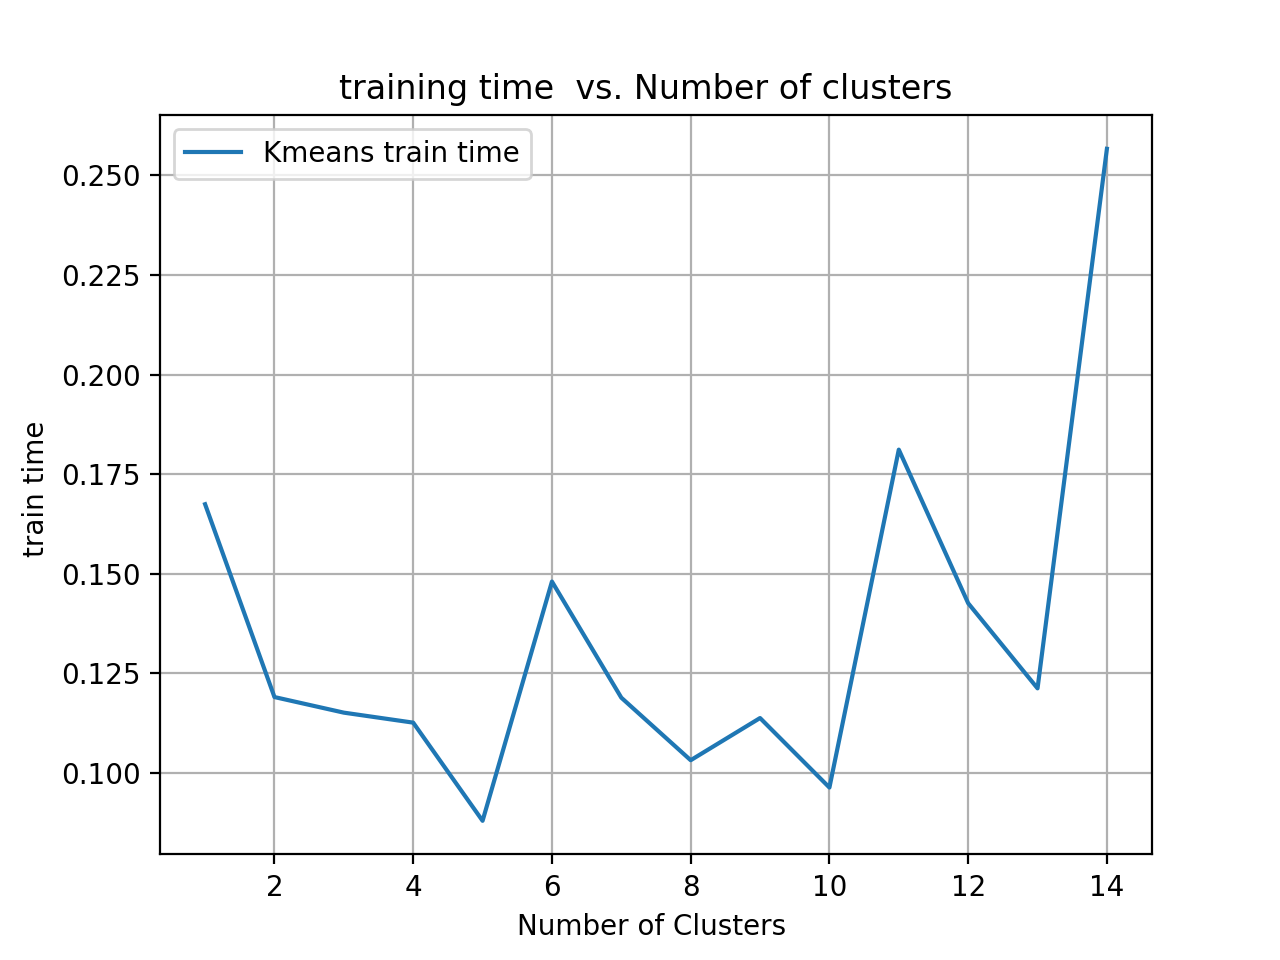
\includegraphics[width=.95\linewidth]{train_time_kmeans_5}
     \end{minipage}\hfill
     \begin{minipage}{0.25\textwidth}
     \centering
     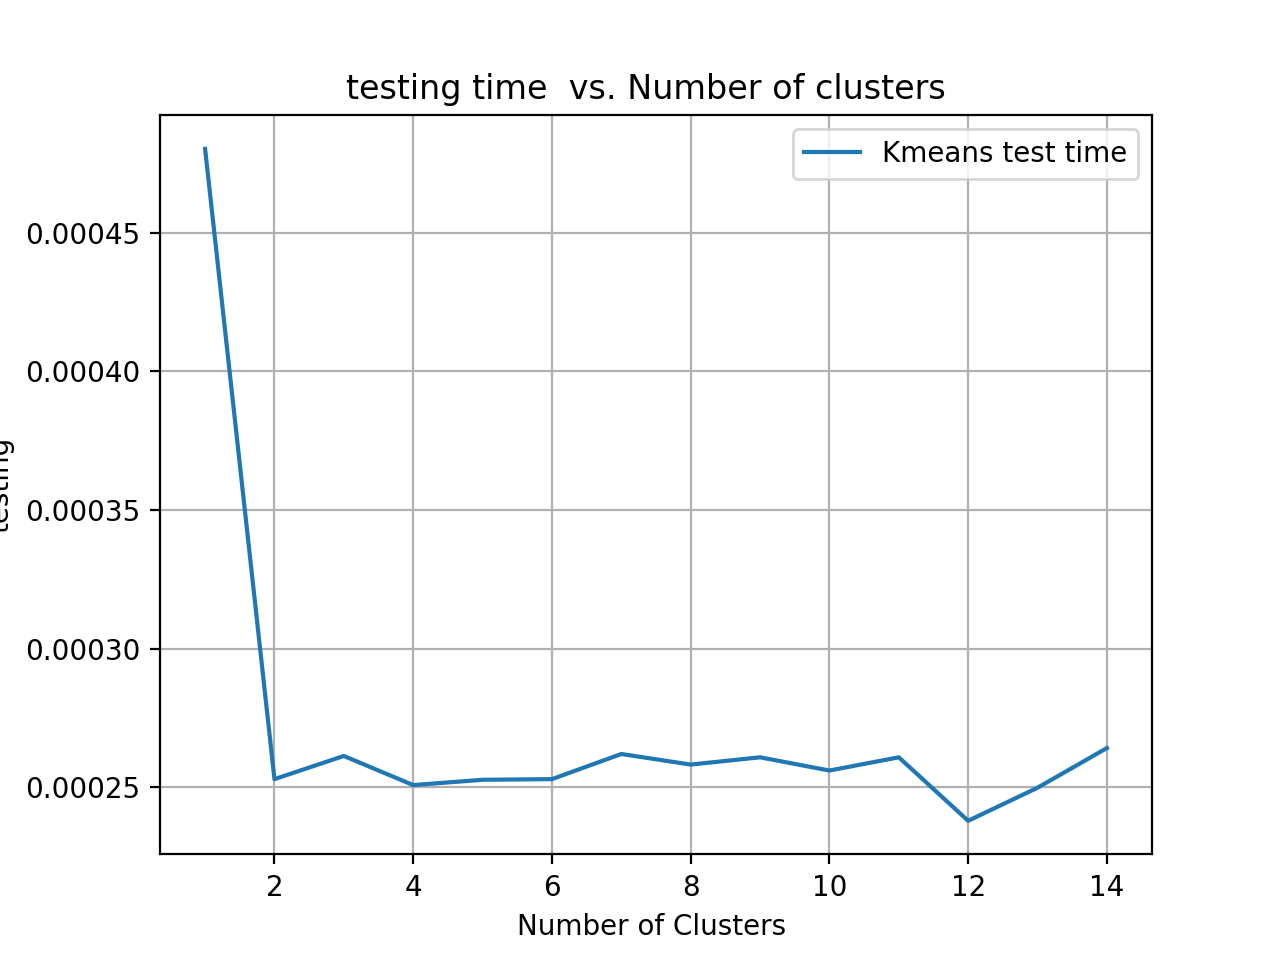
\includegraphics[width=.95\linewidth]{test_time_nn_5}
   \end{minipage}\hfill
    \begin{minipage}{0.25\textwidth}
     \centering
     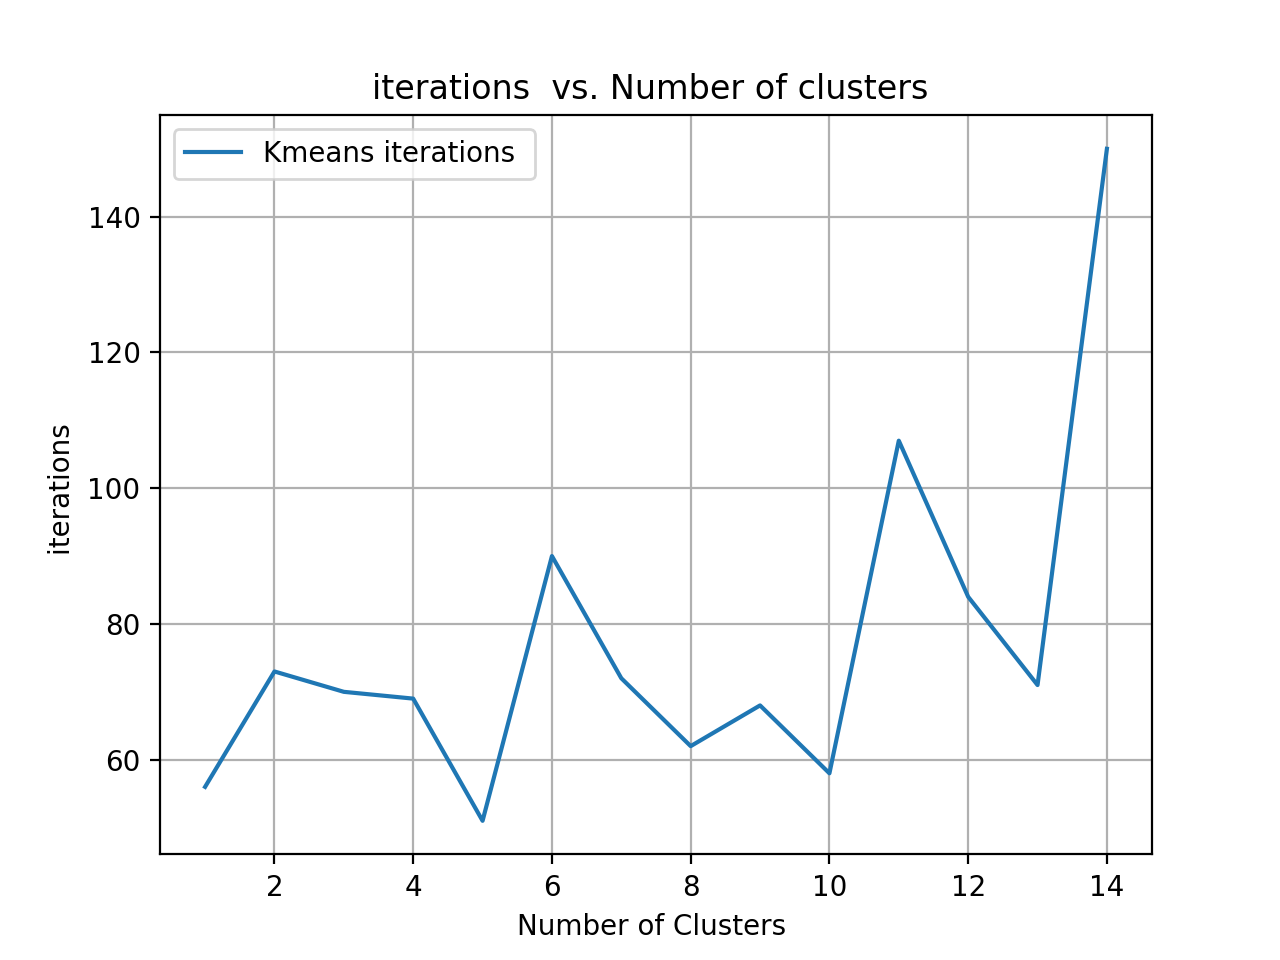
\includegraphics[width=.95\linewidth]{kmeans_iter_nn_5}
   \end{minipage}\hfill
 \caption { Simulated Annealing Tuning}
\end{figure}


\begin{figure}[!htb]
   \begin{minipage}{0.25\textwidth}
     \centering
     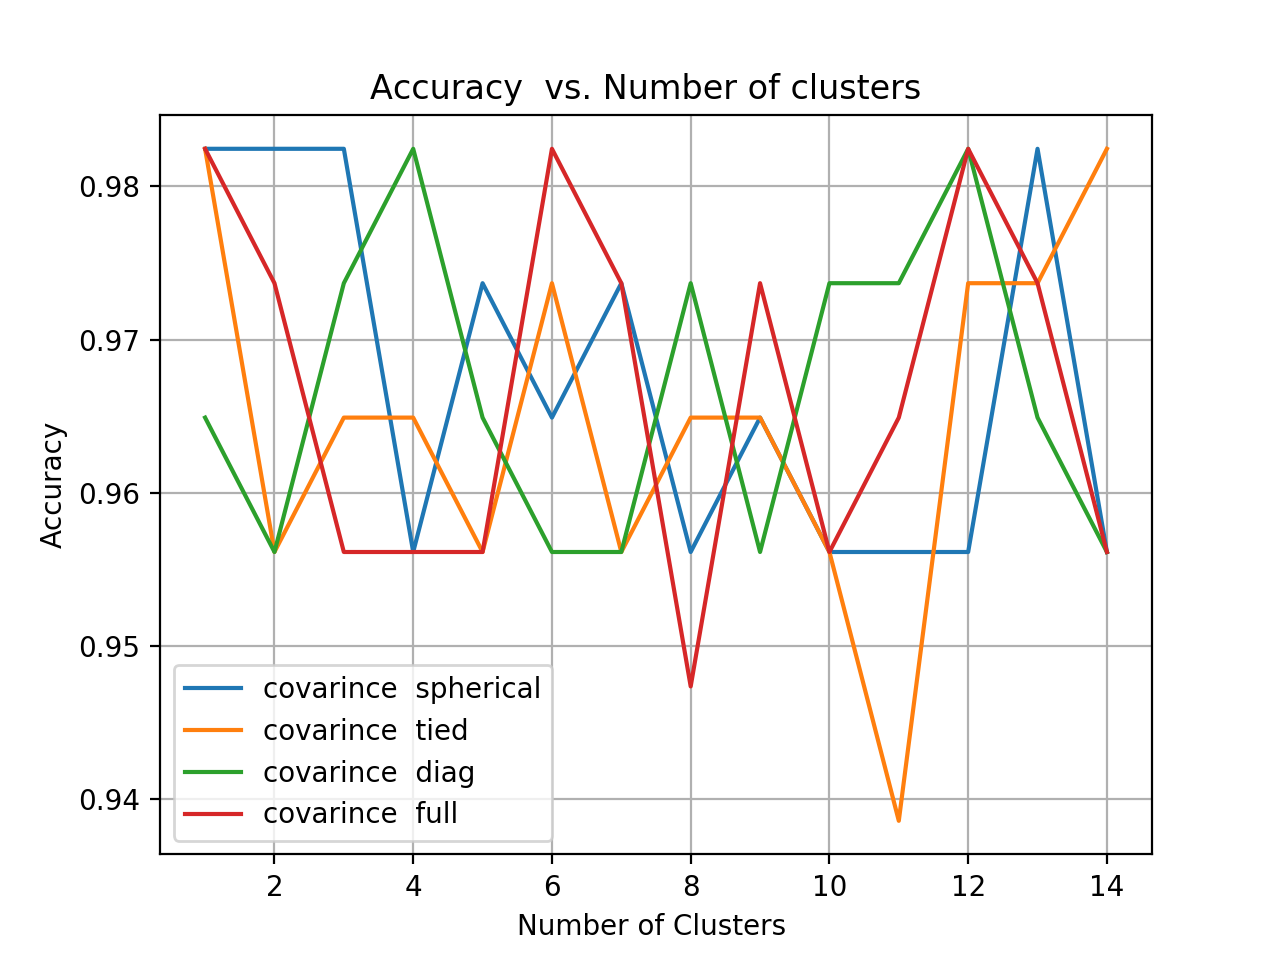
\includegraphics[width=.95\linewidth]{em_acc_nn_5}
   \end{minipage}\hfill
    \begin{minipage}{0.25\textwidth}
     \centering
     \includegraphics[width=.95\linewidth]{em_nn_train_5}
     \end{minipage}\hfill
     \begin{minipage}{0.25\textwidth}
     \centering
     \includegraphics[width=.95\linewidth]{em_test_nn_5}
   \end{minipage}\hfill
    \begin{minipage}{0.25\textwidth}
     \centering
     \includegraphics[width=.95\linewidth]{em_iter_nn_5}
   \end{minipage}\hfill
 \caption { Simulated Annealing Tuning}
\end{figure}


\end{document}
